\documentclass[twoside]{book}

% Packages required by doxygen
\usepackage{fixltx2e}
\usepackage{calc}
\usepackage{doxygen}
\usepackage{graphicx}
\usepackage[utf8]{inputenc}
\usepackage{makeidx}
\usepackage{multicol}
\usepackage{multirow}
\PassOptionsToPackage{warn}{textcomp}
\usepackage{textcomp}
\usepackage[nointegrals]{wasysym}
\usepackage[table]{xcolor}

% NLS support packages
\usepackage[french]{babel}

% Font selection
\usepackage[T1]{fontenc}
\usepackage{mathptmx}
\usepackage[scaled=.90]{helvet}
\usepackage{courier}
\usepackage{amssymb}
\usepackage{sectsty}
\renewcommand{\familydefault}{\sfdefault}
\allsectionsfont{%
  \fontseries{bc}\selectfont%
  \color{darkgray}%
}
\renewcommand{\DoxyLabelFont}{%
  \fontseries{bc}\selectfont%
  \color{darkgray}%
}
\newcommand{\+}{\discretionary{\mbox{\scriptsize$\hookleftarrow$}}{}{}}

% Page & text layout
\usepackage{geometry}
\geometry{%
  a4paper,%
  top=2.5cm,%
  bottom=2.5cm,%
  left=2.5cm,%
  right=2.5cm%
}
\tolerance=750
\hfuzz=15pt
\hbadness=750
\setlength{\emergencystretch}{15pt}
\setlength{\parindent}{0cm}
\setlength{\parskip}{0.2cm}
\makeatletter
\renewcommand{\paragraph}{%
  \@startsection{paragraph}{4}{0ex}{-1.0ex}{1.0ex}{%
    \normalfont\normalsize\bfseries\SS@parafont%
  }%
}
\renewcommand{\subparagraph}{%
  \@startsection{subparagraph}{5}{0ex}{-1.0ex}{1.0ex}{%
    \normalfont\normalsize\bfseries\SS@subparafont%
  }%
}
\makeatother

% Headers & footers
\usepackage{fancyhdr}
\pagestyle{fancyplain}
\fancyhead[LE]{\fancyplain{}{\bfseries\thepage}}
\fancyhead[CE]{\fancyplain{}{}}
\fancyhead[RE]{\fancyplain{}{\bfseries\leftmark}}
\fancyhead[LO]{\fancyplain{}{\bfseries\rightmark}}
\fancyhead[CO]{\fancyplain{}{}}
\fancyhead[RO]{\fancyplain{}{\bfseries\thepage}}
\fancyfoot[LE]{\fancyplain{}{}}
\fancyfoot[CE]{\fancyplain{}{}}
\fancyfoot[RE]{\fancyplain{}{\bfseries\scriptsize Généré le Mercredi 25 Novembre 2015 11\+:59\+:02 pour Projet Design Pattern par Doxygen }}
\fancyfoot[LO]{\fancyplain{}{\bfseries\scriptsize Généré le Mercredi 25 Novembre 2015 11\+:59\+:02 pour Projet Design Pattern par Doxygen }}
\fancyfoot[CO]{\fancyplain{}{}}
\fancyfoot[RO]{\fancyplain{}{}}
\renewcommand{\footrulewidth}{0.4pt}
\renewcommand{\chaptermark}[1]{%
  \markboth{#1}{}%
}
\renewcommand{\sectionmark}[1]{%
  \markright{\thesection\ #1}%
}

% Indices & bibliography
\usepackage{natbib}
\usepackage[titles]{tocloft}
\setcounter{tocdepth}{3}
\setcounter{secnumdepth}{5}
\makeindex

% Hyperlinks (required, but should be loaded last)
\usepackage{ifpdf}
\ifpdf
  \usepackage[pdftex,pagebackref=true]{hyperref}
\else
  \usepackage[ps2pdf,pagebackref=true]{hyperref}
\fi
\hypersetup{%
  colorlinks=true,%
  linkcolor=blue,%
  citecolor=blue,%
  unicode%
}

% Custom commands
\newcommand{\clearemptydoublepage}{%
  \newpage{\pagestyle{empty}\cleardoublepage}%
}


%===== C O N T E N T S =====

\begin{document}

% Titlepage & ToC
\hypersetup{pageanchor=false,
             bookmarks=true,
             bookmarksnumbered=true,
             pdfencoding=unicode
            }
\pagenumbering{roman}
\begin{titlepage}
\vspace*{7cm}
\begin{center}%
{\Large Projet Design Pattern }\\
\vspace*{1cm}
{\large Généré par Doxygen 1.8.7}\\
\vspace*{0.5cm}
{\small Mercredi 25 Novembre 2015 11:59:02}\\
\end{center}
\end{titlepage}
\clearemptydoublepage
\tableofcontents
\clearemptydoublepage
\pagenumbering{arabic}
\hypersetup{pageanchor=true}

%--- Begin generated contents ---
\chapter{Index hiérarchique}
\section{Hiérarchie des classes}
Cette liste d'héritage est classée approximativement par ordre alphabétique \+:\begin{DoxyCompactList}
\item \contentsline{section}{Attack}{\pageref{classAttack}}{}
\begin{DoxyCompactList}
\item \contentsline{section}{Concrete\+Base\+Attack}{\pageref{classConcreteBaseAttack}}{}
\item \contentsline{section}{Concrete\+Base\+Attack\+Spe\+Base}{\pageref{classConcreteBaseAttackSpeBase}}{}
\end{DoxyCompactList}
\item \contentsline{section}{Base}{\pageref{classBase}}{}
\item \contentsline{section}{Concrete\+Concrete\+H\+P\+Loss}{\pageref{classConcreteConcreteHPLoss}}{}
\item \contentsline{section}{Concrete\+Concrete\+H\+P\+Loss\+Spe\+Def}{\pageref{classConcreteConcreteHPLossSpeDef}}{}
\item \contentsline{section}{Data}{\pageref{classData}}{}
\item Drawable\begin{DoxyCompactList}
\item \contentsline{section}{Tile\+Map}{\pageref{classTileMap}}{}
\end{DoxyCompactList}
\item \contentsline{section}{H\+P\+Loss}{\pageref{classHPLoss}}{}
\begin{DoxyCompactList}
\item \contentsline{section}{Concrete\+H\+P\+Loss}{\pageref{classConcreteHPLoss}}{}
\item \contentsline{section}{Concrete\+H\+P\+Loss\+Spe\+Def}{\pageref{classConcreteHPLossSpeDef}}{}
\end{DoxyCompactList}
\item \contentsline{section}{Map}{\pageref{classMap}}{}
\item \contentsline{section}{Move}{\pageref{classMove}}{}
\begin{DoxyCompactList}
\item \contentsline{section}{Concrete\+Move}{\pageref{classConcreteMove}}{}
\end{DoxyCompactList}
\item \contentsline{section}{Observer}{\pageref{classObserver}}{}
\begin{DoxyCompactList}
\item \contentsline{section}{Window}{\pageref{classWindow}}{}
\end{DoxyCompactList}
\item \contentsline{section}{Observeur}{\pageref{classObserveur}}{}
\item \contentsline{section}{Path}{\pageref{classPath}}{}
\item \contentsline{section}{Player}{\pageref{classPlayer}}{}
\item \contentsline{section}{Position}{\pageref{classPosition}}{}
\item \contentsline{section}{Spawner}{\pageref{classSpawner}}{}
\item \contentsline{section}{Subject}{\pageref{classSubject}}{}
\begin{DoxyCompactList}
\item \contentsline{section}{Game}{\pageref{classGame}}{}
\end{DoxyCompactList}
\item Transformable\begin{DoxyCompactList}
\item \contentsline{section}{Tile\+Map}{\pageref{classTileMap}}{}
\end{DoxyCompactList}
\item \contentsline{section}{Unit}{\pageref{classUnit}}{}
\begin{DoxyCompactList}
\item \contentsline{section}{Archer}{\pageref{classArcher}}{}
\item \contentsline{section}{Knight}{\pageref{classKnight}}{}
\end{DoxyCompactList}
\end{DoxyCompactList}

\chapter{Index des classes}
\section{Liste des classes}
Liste des classes, structures, unions et interfaces avec une brève description \+:\begin{DoxyCompactList}
\item\contentsline{section}{\hyperlink{classArcher}{Archer} \\*Classe définissant un archer }{\pageref{classArcher}}{}
\item\contentsline{section}{\hyperlink{classAttack}{Attack} \\*Classe virtuelle pure permettant l'utilisation de différents comportement d'attaque selon l'unité. Elle est utilisée dans le cadre du pattern Strategy }{\pageref{classAttack}}{}
\item\contentsline{section}{\hyperlink{classBase}{Base} \\*Classe définissant une base }{\pageref{classBase}}{}
\item\contentsline{section}{\hyperlink{classConcreteBaseAttack}{Concrete\+Base\+Attack} \\*Classe concrete définissant le comportement d'attaque de base des unités normales }{\pageref{classConcreteBaseAttack}}{}
\item\contentsline{section}{\hyperlink{classConcreteBaseAttackSpeBase}{Concrete\+Base\+Attack\+Spe\+Base} }{\pageref{classConcreteBaseAttackSpeBase}}{}
\item\contentsline{section}{\hyperlink{classConcreteConcreteHPLoss}{Concrete\+Concrete\+H\+P\+Loss} \\*Classe concrete définissant le comportement de la perte de point de vie des unités normales }{\pageref{classConcreteConcreteHPLoss}}{}
\item\contentsline{section}{\hyperlink{classConcreteConcreteHPLossSpeDef}{Concrete\+Concrete\+H\+P\+Loss\+Spe\+Def} \\*Classe concrete définissant le comportement de la perte de point de vie des unités défensives }{\pageref{classConcreteConcreteHPLossSpeDef}}{}
\item\contentsline{section}{\hyperlink{classConcreteHPLoss}{Concrete\+H\+P\+Loss} }{\pageref{classConcreteHPLoss}}{}
\item\contentsline{section}{\hyperlink{classConcreteHPLossSpeDef}{Concrete\+H\+P\+Loss\+Spe\+Def} }{\pageref{classConcreteHPLossSpeDef}}{}
\item\contentsline{section}{\hyperlink{classConcreteMove}{Concrete\+Move} \\*Classe concrete définissant le comportement de déplacement des unités mouvantes }{\pageref{classConcreteMove}}{}
\item\contentsline{section}{\hyperlink{classData}{Data} \\*Classe qui centralise toute les données du jeu }{\pageref{classData}}{}
\item\contentsline{section}{\hyperlink{classGame}{Game} \\*Classe qui centralisera tout le jeu }{\pageref{classGame}}{}
\item\contentsline{section}{\hyperlink{classHPLoss}{H\+P\+Loss} \\*Classe virtuelle pure permettant l'utilisation de différents comportement de la perte de points de vie selon l'unité. Elle est utilisée dans le cadre du pattern Strategy }{\pageref{classHPLoss}}{}
\item\contentsline{section}{\hyperlink{classKnight}{Knight} \\*Classe définissant un chevalier }{\pageref{classKnight}}{}
\item\contentsline{section}{\hyperlink{classMap}{Map} \\*Classe permettant l'utilisation d'une map }{\pageref{classMap}}{}
\item\contentsline{section}{\hyperlink{classMove}{Move} \\*Classe virtuelle pure permettant l'utilisation de différents comportement de déplacements selon l'unité. Elle est utilisée dans le cadre du pattern Strategy }{\pageref{classMove}}{}
\item\contentsline{section}{\hyperlink{classObserver}{Observer} }{\pageref{classObserver}}{}
\item\contentsline{section}{\hyperlink{classObserveur}{Observeur} \\*Classe abstraite définissant le comportement des toutes les classes observatrices }{\pageref{classObserveur}}{}
\item\contentsline{section}{\hyperlink{classPath}{Path} \\*Classe implémentant un chemin (path) sur la map }{\pageref{classPath}}{}
\item\contentsline{section}{\hyperlink{classPlayer}{Player} \\*Classe définissant un joueur }{\pageref{classPlayer}}{}
\item\contentsline{section}{\hyperlink{classPosition}{Position} \\*Classe implémentant une position sur la map }{\pageref{classPosition}}{}
\item\contentsline{section}{\hyperlink{classSpawner}{Spawner} \\*Classe permettant l'utilisation des spawner (générateur d'unités) }{\pageref{classSpawner}}{}
\item\contentsline{section}{\hyperlink{classSubject}{Subject} \\*Classe abstraite définissant le comportement des toutes les classes sujets }{\pageref{classSubject}}{}
\item\contentsline{section}{\hyperlink{classTileMap}{Tile\+Map} \\*Affichage d'une map }{\pageref{classTileMap}}{}
\item\contentsline{section}{\hyperlink{classUnit}{Unit} \\*Classe permettant l'utilisation d'unités }{\pageref{classUnit}}{}
\item\contentsline{section}{\hyperlink{classWindow}{Window} \\*Affichage d'une fenêtre }{\pageref{classWindow}}{}
\end{DoxyCompactList}

\chapter{Index des fichiers}
\section{Liste des fichiers}
Liste de tous les fichiers documentés avec une brève description \+:\begin{DoxyCompactList}
\item\contentsline{section}{src/\hyperlink{archer_8hpp}{archer.\+hpp} \\*Définition de la classe \hyperlink{classArcher}{Archer} }{\pageref{archer_8hpp}}{}
\item\contentsline{section}{src/\hyperlink{attack_8hpp}{attack.\+hpp} \\*Définition des stratégies d'attaque }{\pageref{attack_8hpp}}{}
\item\contentsline{section}{src/\hyperlink{base_8hpp}{base.\+hpp} \\*Définition de la classe \hyperlink{classBase}{Base} }{\pageref{base_8hpp}}{}
\item\contentsline{section}{src/\hyperlink{concreteBaseAttack_8hpp}{concrete\+Base\+Attack.\+hpp} \\*Définition de l'attaque de base normale }{\pageref{concreteBaseAttack_8hpp}}{}
\item\contentsline{section}{src/\hyperlink{concreteBaseAttackSpeBase_8hpp}{concrete\+Base\+Attack\+Spe\+Base.\+hpp} \\*Définition de l'attaque de base pour les unité puissante sur les bases }{\pageref{concreteBaseAttackSpeBase_8hpp}}{}
\item\contentsline{section}{src/\hyperlink{concretehploss_8hpp}{concretehploss.\+hpp} \\*Définition de la perte d'H\+P de base }{\pageref{concretehploss_8hpp}}{}
\item\contentsline{section}{src/\hyperlink{concretehplossspedef_8hpp}{concretehplossspedef.\+hpp} \\*Définition de la perte d'H\+P d'une unité défensive }{\pageref{concretehplossspedef_8hpp}}{}
\item\contentsline{section}{src/\hyperlink{concretemove_8hpp}{concretemove.\+hpp} \\*Définition du mouvement }{\pageref{concretemove_8hpp}}{}
\item\contentsline{section}{src/\hyperlink{data_8hpp}{data.\+hpp} \\*Définition de la classe data }{\pageref{data_8hpp}}{}
\item\contentsline{section}{src/\hyperlink{game_8hpp}{game.\+hpp} \\*Définition de la classe game }{\pageref{game_8hpp}}{}
\item\contentsline{section}{src/\hyperlink{hploss_8hpp}{hploss.\+hpp} \\*Définition du comportement de la perte d'H\+P }{\pageref{hploss_8hpp}}{}
\item\contentsline{section}{src/\hyperlink{knight_8hpp}{knight.\+hpp} \\*Définition de la classe \hyperlink{classKnight}{Knight} }{\pageref{knight_8hpp}}{}
\item\contentsline{section}{src/\hyperlink{map_8hpp}{map.\+hpp} \\*Définition de la classe \hyperlink{classMap}{Map} }{\pageref{map_8hpp}}{}
\item\contentsline{section}{src/\hyperlink{move_8hpp}{move.\+hpp} \\*Définition des stratégies de déplacement }{\pageref{move_8hpp}}{}
\item\contentsline{section}{src/\hyperlink{observer_8hpp}{observer.\+hpp} \\*Définition de la classe abstraite observateur }{\pageref{observer_8hpp}}{}
\item\contentsline{section}{src/\hyperlink{path_8hpp}{path.\+hpp} \\*Definition de la classe \hyperlink{classPath}{Path} }{\pageref{path_8hpp}}{}
\item\contentsline{section}{src/\hyperlink{player_8hpp}{player.\+hpp} \\*Définition de la classe \hyperlink{classPlayer}{Player} }{\pageref{player_8hpp}}{}
\item\contentsline{section}{src/\hyperlink{position_8hpp}{position.\+hpp} \\*Definition de la classe \hyperlink{classPosition}{Position} }{\pageref{position_8hpp}}{}
\item\contentsline{section}{src/\hyperlink{spawner_8hpp}{spawner.\+hpp} \\*Définition de la classe \hyperlink{classSpawner}{Spawner} }{\pageref{spawner_8hpp}}{}
\item\contentsline{section}{src/\hyperlink{subject_8hpp}{subject.\+hpp} \\*Définition de la classe abstraite sujet }{\pageref{subject_8hpp}}{}
\item\contentsline{section}{src/\hyperlink{tilemap_8hpp}{tilemap.\+hpp} \\*Définition de la classe qui crée la map graphique }{\pageref{tilemap_8hpp}}{}
\item\contentsline{section}{src/\hyperlink{unit_8hpp}{unit.\+hpp} \\*Définition de la classe \hyperlink{classUnit}{Unit} }{\pageref{unit_8hpp}}{}
\item\contentsline{section}{src/\hyperlink{window_8hpp}{window.\+hpp} \\*Définition de la classe d'affichage }{\pageref{window_8hpp}}{}
\end{DoxyCompactList}

\chapter{Documentation des classes}
\hypertarget{classArcher}{\section{Référence de la classe Archer}
\label{classArcher}\index{Archer@{Archer}}
}


Classe définissant un archer.  




{\ttfamily \#include $<$archer.\+hpp$>$}

Graphe d'héritage de Archer\+:\begin{figure}[H]
\begin{center}
\leavevmode
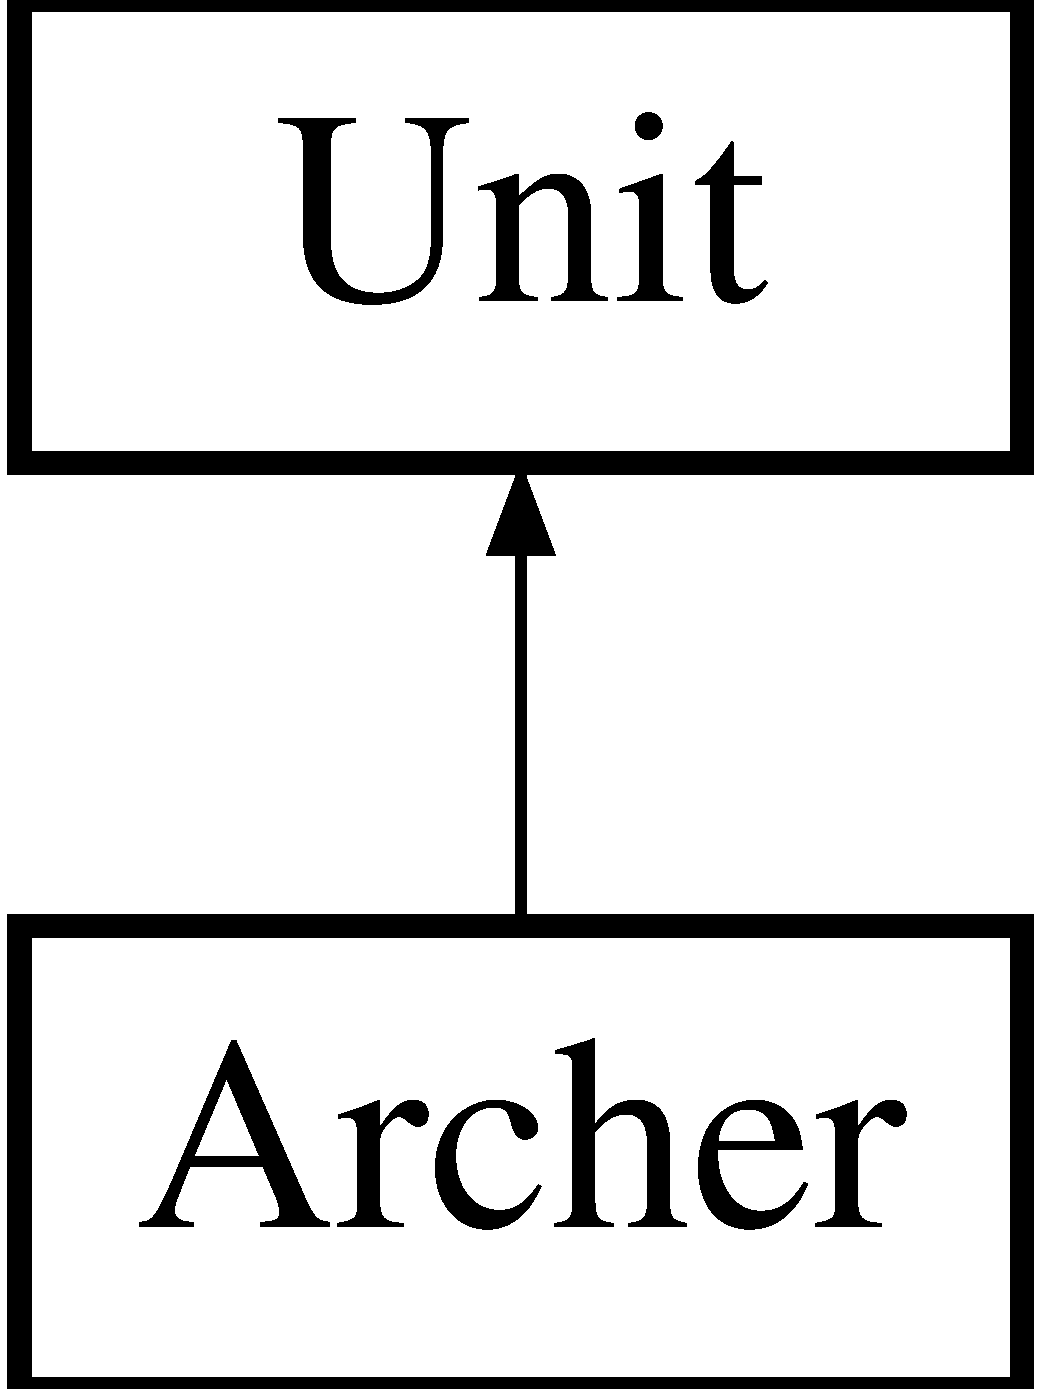
\includegraphics[height=2.000000cm]{classArcher}
\end{center}
\end{figure}
\subsection*{Fonctions membres publiques}
\begin{DoxyCompactItemize}
\item 
\hypertarget{classArcher_a339791774caa50d6a8d3a5b7a10fb228}{\hyperlink{classArcher_a339791774caa50d6a8d3a5b7a10fb228}{Archer} (unsigned int range, unsigned int ap, unsigned int mp, unsigned int hp, unsigned int dmgs, unsigned int cost, \hyperlink{classAttack}{Attack} $\ast$\hyperlink{classUnit_ac06b8f6e30f851f15a42d8a1d951034a}{attack}, \hyperlink{classHPLoss}{H\+P\+Loss} $\ast$\hyperlink{classUnit_a3090f43e2ee6a08587a160afaa26e7cd}{hp\+Loss}, \hyperlink{classMove}{Move} $\ast$\hyperlink{classUnit_a8c6bfbaf9bf204baec6ba3c11468ec2f}{move}, \hyperlink{classPosition}{Position} position, std\+::string image)}\label{classArcher_a339791774caa50d6a8d3a5b7a10fb228}

\begin{DoxyCompactList}\small\item\em Constructeur. \end{DoxyCompactList}\item 
std\+::string \hyperlink{classArcher_a41ff30d3d1eac71a13bd5b5cc86a2d6b}{classe} () const 
\begin{DoxyCompactList}\small\item\em Accesseur de la classe. \end{DoxyCompactList}\item 
\hyperlink{classUnit}{Unit} $\ast$ \hyperlink{classArcher_a898839f83f972b3e2c000c9dfb92487c}{clone} (\hyperlink{classPosition}{Position} position) const 
\begin{DoxyCompactList}\small\item\em construit un archer identique à la position donnée \end{DoxyCompactList}\item 
\hypertarget{classArcher_a711fbb1d20af0d71b68e35b41507615b}{void \hyperlink{classArcher_a711fbb1d20af0d71b68e35b41507615b}{afficher\+Infos} () const }\label{classArcher_a711fbb1d20af0d71b68e35b41507615b}

\begin{DoxyCompactList}\small\item\em affiche les différentes informations sur l'archer \end{DoxyCompactList}\end{DoxyCompactItemize}
\subsection*{Membres hérités additionnels}


\subsection{Description détaillée}
Classe définissant un archer. 

Définition à la ligne 20 du fichier archer.\+hpp.



\subsection{Documentation des fonctions membres}
\hypertarget{classArcher_a41ff30d3d1eac71a13bd5b5cc86a2d6b}{\index{Archer@{Archer}!classe@{classe}}
\index{classe@{classe}!Archer@{Archer}}
\subsubsection[{classe}]{\setlength{\rightskip}{0pt plus 5cm}std\+::string Archer\+::classe (
\begin{DoxyParamCaption}
{}
\end{DoxyParamCaption}
) const\hspace{0.3cm}{\ttfamily [virtual]}}}\label{classArcher_a41ff30d3d1eac71a13bd5b5cc86a2d6b}


Accesseur de la classe. 

\begin{DoxyReturn}{Renvoie}
\char`\"{}archer\char`\"{} 
\end{DoxyReturn}


Implémente \hyperlink{classUnit_adac07557f9c0b9005709c62263625c2d}{Unit}.

\hypertarget{classArcher_a898839f83f972b3e2c000c9dfb92487c}{\index{Archer@{Archer}!clone@{clone}}
\index{clone@{clone}!Archer@{Archer}}
\subsubsection[{clone}]{\setlength{\rightskip}{0pt plus 5cm}{\bf Unit}$\ast$ Archer\+::clone (
\begin{DoxyParamCaption}
\item[{{\bf Position}}]{position}
\end{DoxyParamCaption}
) const\hspace{0.3cm}{\ttfamily [virtual]}}}\label{classArcher_a898839f83f972b3e2c000c9dfb92487c}


construit un archer identique à la position donnée 


\begin{DoxyParams}{Paramètres}
{\em position} & une position \\
\hline
\end{DoxyParams}
\begin{DoxyReturn}{Renvoie}
un archer 
\end{DoxyReturn}


Implémente \hyperlink{classUnit_a90304713be4b7cc73f59358190dd39d4}{Unit}.



La documentation de cette classe a été générée à partir du fichier suivant \+:\begin{DoxyCompactItemize}
\item 
src/\hyperlink{archer_8hpp}{archer.\+hpp}\end{DoxyCompactItemize}

\hypertarget{classAttack}{\section{Référence de la classe Attack}
\label{classAttack}\index{Attack@{Attack}}
}


Classe virtuelle pure permettant l'utilisation de différents comportement d'attaque selon l'unité. Elle est utilisée dans le cadre du pattern Strategy.  




{\ttfamily \#include $<$attack.\+hpp$>$}

Graphe d'héritage de Attack\+:\begin{figure}[H]
\begin{center}
\leavevmode
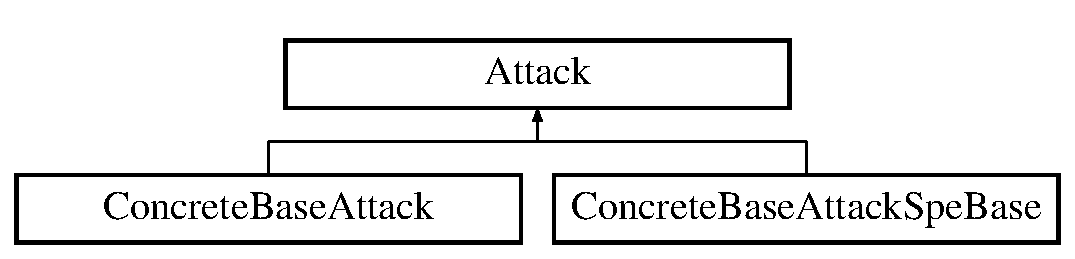
\includegraphics[height=2.000000cm]{classAttack}
\end{center}
\end{figure}
\subsection*{Fonctions membres publiques}
\begin{DoxyCompactItemize}
\item 
\hypertarget{classAttack_ab7a4ca023e07dd3c94ea31c081046f9e}{\hyperlink{classAttack_ab7a4ca023e07dd3c94ea31c081046f9e}{Attack} (unsigned int ap)}\label{classAttack_ab7a4ca023e07dd3c94ea31c081046f9e}

\begin{DoxyCompactList}\small\item\em Constructeur. \end{DoxyCompactList}\item 
virtual void \hyperlink{classAttack_aa741caafef0d80bb0a00ce39e5bf6e2d}{attack} (\hyperlink{classPosition}{Position} position, \hyperlink{classMap}{Map} $\ast$map, \hyperlink{classUnit}{Unit} $\ast$attacker)=0
\begin{DoxyCompactList}\small\item\em Destructeur (évite les warnings) \end{DoxyCompactList}\end{DoxyCompactItemize}
\subsection*{Attributs protégés}
\begin{DoxyCompactItemize}
\item 
\hypertarget{classAttack_a33e2aea32bc58913dbde9f66bcadf981}{unsigned int {\bfseries \+\_\+ap}}\label{classAttack_a33e2aea32bc58913dbde9f66bcadf981}

\end{DoxyCompactItemize}


\subsection{Description détaillée}
Classe virtuelle pure permettant l'utilisation de différents comportement d'attaque selon l'unité. Elle est utilisée dans le cadre du pattern Strategy. 

Définition à la ligne 21 du fichier attack.\+hpp.



\subsection{Documentation des fonctions membres}
\hypertarget{classAttack_aa741caafef0d80bb0a00ce39e5bf6e2d}{\index{Attack@{Attack}!attack@{attack}}
\index{attack@{attack}!Attack@{Attack}}
\subsubsection[{attack}]{\setlength{\rightskip}{0pt plus 5cm}virtual void Attack\+::attack (
\begin{DoxyParamCaption}
\item[{{\bf Position}}]{position, }
\item[{{\bf Map} $\ast$}]{map, }
\item[{{\bf Unit} $\ast$}]{attacker}
\end{DoxyParamCaption}
)\hspace{0.3cm}{\ttfamily [pure virtual]}}}\label{classAttack_aa741caafef0d80bb0a00ce39e5bf6e2d}


Destructeur (évite les warnings) 

Méthode virtuelle pure d'attaque 
\begin{DoxyParams}{Paramètres}
{\em position} & une position \\
\hline
{\em map} & une map \\
\hline
{\em attacker} & l'unité qui attaque \\
\hline
\end{DoxyParams}


Implémenté dans \hyperlink{classConcreteBaseAttack_a35cf2248ae6a719ba6041f95ea1428a2}{Concrete\+Base\+Attack}, et \hyperlink{classConcreteBaseAttackSpeBase_a4b215e51d3146516ecf77e23d19a92de}{Concrete\+Base\+Attack\+Spe\+Base}.



La documentation de cette classe a été générée à partir du fichier suivant \+:\begin{DoxyCompactItemize}
\item 
src/\hyperlink{attack_8hpp}{attack.\+hpp}\end{DoxyCompactItemize}

\hypertarget{classBase}{\section{Référence de la classe Base}
\label{classBase}\index{Base@{Base}}
}


Classe définissant une base.  




{\ttfamily \#include $<$base.\+hpp$>$}

\subsection*{Fonctions membres publiques}
\begin{DoxyCompactItemize}
\item 
\hypertarget{classBase_a32aefb7f04339edda2e2517502dd27b2}{\hyperlink{classBase_a32aefb7f04339edda2e2517502dd27b2}{Base} (unsigned int hp, unsigned int summon\+Range, unsigned int build\+Range, \hyperlink{classHPLoss}{H\+P\+Loss} $\ast$\hyperlink{classBase_a3f6ba779a531b048daa9cec42c945b91}{hp\+Loss}, \hyperlink{classPosition}{Position} position)}\label{classBase_a32aefb7f04339edda2e2517502dd27b2}

\begin{DoxyCompactList}\small\item\em Constructeur. \end{DoxyCompactList}\item 
\hypertarget{classBase_a722da881b6c70cfcbde9243abcfbf334}{\hyperlink{classBase_a722da881b6c70cfcbde9243abcfbf334}{$\sim$\+Base} ()}\label{classBase_a722da881b6c70cfcbde9243abcfbf334}

\begin{DoxyCompactList}\small\item\em Destructeur. \end{DoxyCompactList}\item 
unsigned int \hyperlink{classBase_a7f6a0b45ce6331d7bfb0d6f716d5ba60}{get\+Summon\+Range} () const 
\begin{DoxyCompactList}\small\item\em Accesseur de la portée d'invocation. \end{DoxyCompactList}\item 
unsigned int \hyperlink{classBase_a1bd08f26289caa9aa0028efd9dae8d9e}{get\+Build\+Range} () const 
\begin{DoxyCompactList}\small\item\em Accesseur de la portée de construction. \end{DoxyCompactList}\item 
\hypertarget{classBase_a1a3daeb406afce579a88debf4424b0a0}{void \hyperlink{classBase_a1a3daeb406afce579a88debf4424b0a0}{afficher} () const }\label{classBase_a1a3daeb406afce579a88debf4424b0a0}

\begin{DoxyCompactList}\small\item\em Affiche la base. \end{DoxyCompactList}\item 
void \hyperlink{classBase_a0e05c8081bb85324b884abfa6712f6fb}{set\+H\+P} (unsigned int value)
\begin{DoxyCompactList}\small\item\em Modificateur du nombre de points de vie. \end{DoxyCompactList}\item 
unsigned int \hyperlink{classBase_a8fd6606cff73e39cd05225bd7b395218}{get\+H\+P} () const 
\begin{DoxyCompactList}\small\item\em Accesseur des points de vie. \end{DoxyCompactList}\item 
unsigned int \hyperlink{classBase_a8599d1b3c4d1b744d5e3d42abfb47361}{get\+Max\+H\+P} () const 
\begin{DoxyCompactList}\small\item\em Accesseur des points de vie max. \end{DoxyCompactList}\item 
void \hyperlink{classBase_a0e2dd85f633ed25b9ab144fb7c769b7b}{set\+Player} (\hyperlink{classPlayer}{Player} $\ast$player)
\begin{DoxyCompactList}\small\item\em Modificateur du joueur associé à la base. \end{DoxyCompactList}\item 
\hyperlink{classPosition}{Position} \hyperlink{classBase_ae2abb880ce9543ac70419714f8c1181f}{get\+Position} () const 
\begin{DoxyCompactList}\small\item\em Accesseur de la position de la base. \end{DoxyCompactList}\item 
void \hyperlink{classBase_a17fc3f12f7aedbf5a8be8f0f271a3f62}{set\+Position} (\hyperlink{classPosition}{Position} position)
\begin{DoxyCompactList}\small\item\em Modificateur de la position de la base. \end{DoxyCompactList}\item 
void \hyperlink{classBase_a3f6ba779a531b048daa9cec42c945b91}{hp\+Loss} (unsigned int value)
\begin{DoxyCompactList}\small\item\em L'unité perd des points de vie. \end{DoxyCompactList}\end{DoxyCompactItemize}


\subsection{Description détaillée}
Classe définissant une base. 

Définition à la ligne 21 du fichier base.\+hpp.



\subsection{Documentation des fonctions membres}
\hypertarget{classBase_a1bd08f26289caa9aa0028efd9dae8d9e}{\index{Base@{Base}!get\+Build\+Range@{get\+Build\+Range}}
\index{get\+Build\+Range@{get\+Build\+Range}!Base@{Base}}
\subsubsection[{get\+Build\+Range}]{\setlength{\rightskip}{0pt plus 5cm}unsigned int Base\+::get\+Build\+Range (
\begin{DoxyParamCaption}
{}
\end{DoxyParamCaption}
) const}}\label{classBase_a1bd08f26289caa9aa0028efd9dae8d9e}


Accesseur de la portée de construction. 

\begin{DoxyReturn}{Renvoie}
La portée de construction de la base 
\end{DoxyReturn}
\hypertarget{classBase_a8fd6606cff73e39cd05225bd7b395218}{\index{Base@{Base}!get\+H\+P@{get\+H\+P}}
\index{get\+H\+P@{get\+H\+P}!Base@{Base}}
\subsubsection[{get\+H\+P}]{\setlength{\rightskip}{0pt plus 5cm}unsigned int Base\+::get\+H\+P (
\begin{DoxyParamCaption}
{}
\end{DoxyParamCaption}
) const}}\label{classBase_a8fd6606cff73e39cd05225bd7b395218}


Accesseur des points de vie. 

\begin{DoxyReturn}{Renvoie}
le nombre de pdv 
\end{DoxyReturn}
\hypertarget{classBase_a8599d1b3c4d1b744d5e3d42abfb47361}{\index{Base@{Base}!get\+Max\+H\+P@{get\+Max\+H\+P}}
\index{get\+Max\+H\+P@{get\+Max\+H\+P}!Base@{Base}}
\subsubsection[{get\+Max\+H\+P}]{\setlength{\rightskip}{0pt plus 5cm}unsigned int Base\+::get\+Max\+H\+P (
\begin{DoxyParamCaption}
{}
\end{DoxyParamCaption}
) const}}\label{classBase_a8599d1b3c4d1b744d5e3d42abfb47361}


Accesseur des points de vie max. 

\begin{DoxyReturn}{Renvoie}
le nombre de pdv max 
\end{DoxyReturn}
\hypertarget{classBase_ae2abb880ce9543ac70419714f8c1181f}{\index{Base@{Base}!get\+Position@{get\+Position}}
\index{get\+Position@{get\+Position}!Base@{Base}}
\subsubsection[{get\+Position}]{\setlength{\rightskip}{0pt plus 5cm}{\bf Position} Base\+::get\+Position (
\begin{DoxyParamCaption}
{}
\end{DoxyParamCaption}
) const}}\label{classBase_ae2abb880ce9543ac70419714f8c1181f}


Accesseur de la position de la base. 

\begin{DoxyReturn}{Renvoie}
la position 
\end{DoxyReturn}
\hypertarget{classBase_a7f6a0b45ce6331d7bfb0d6f716d5ba60}{\index{Base@{Base}!get\+Summon\+Range@{get\+Summon\+Range}}
\index{get\+Summon\+Range@{get\+Summon\+Range}!Base@{Base}}
\subsubsection[{get\+Summon\+Range}]{\setlength{\rightskip}{0pt plus 5cm}unsigned int Base\+::get\+Summon\+Range (
\begin{DoxyParamCaption}
{}
\end{DoxyParamCaption}
) const}}\label{classBase_a7f6a0b45ce6331d7bfb0d6f716d5ba60}


Accesseur de la portée d'invocation. 

\begin{DoxyReturn}{Renvoie}
La portée d'invocation de la base 
\end{DoxyReturn}
\hypertarget{classBase_a3f6ba779a531b048daa9cec42c945b91}{\index{Base@{Base}!hp\+Loss@{hp\+Loss}}
\index{hp\+Loss@{hp\+Loss}!Base@{Base}}
\subsubsection[{hp\+Loss}]{\setlength{\rightskip}{0pt plus 5cm}void Base\+::hp\+Loss (
\begin{DoxyParamCaption}
\item[{unsigned int}]{value}
\end{DoxyParamCaption}
)}}\label{classBase_a3f6ba779a531b048daa9cec42c945b91}


L'unité perd des points de vie. 


\begin{DoxyParams}{Paramètres}
{\em value} & Le nomdre d'H\+P perdus \\
\hline
\end{DoxyParams}
\hypertarget{classBase_a0e05c8081bb85324b884abfa6712f6fb}{\index{Base@{Base}!set\+H\+P@{set\+H\+P}}
\index{set\+H\+P@{set\+H\+P}!Base@{Base}}
\subsubsection[{set\+H\+P}]{\setlength{\rightskip}{0pt plus 5cm}void Base\+::set\+H\+P (
\begin{DoxyParamCaption}
\item[{unsigned int}]{value}
\end{DoxyParamCaption}
)}}\label{classBase_a0e05c8081bb85324b884abfa6712f6fb}


Modificateur du nombre de points de vie. 


\begin{DoxyParams}{Paramètres}
{\em value} & la nouvelle valeur \\
\hline
\end{DoxyParams}
\hypertarget{classBase_a0e2dd85f633ed25b9ab144fb7c769b7b}{\index{Base@{Base}!set\+Player@{set\+Player}}
\index{set\+Player@{set\+Player}!Base@{Base}}
\subsubsection[{set\+Player}]{\setlength{\rightskip}{0pt plus 5cm}void Base\+::set\+Player (
\begin{DoxyParamCaption}
\item[{{\bf Player} $\ast$}]{player}
\end{DoxyParamCaption}
)}}\label{classBase_a0e2dd85f633ed25b9ab144fb7c769b7b}


Modificateur du joueur associé à la base. 


\begin{DoxyParams}{Paramètres}
{\em player} & le joueur \\
\hline
\end{DoxyParams}
\hypertarget{classBase_a17fc3f12f7aedbf5a8be8f0f271a3f62}{\index{Base@{Base}!set\+Position@{set\+Position}}
\index{set\+Position@{set\+Position}!Base@{Base}}
\subsubsection[{set\+Position}]{\setlength{\rightskip}{0pt plus 5cm}void Base\+::set\+Position (
\begin{DoxyParamCaption}
\item[{{\bf Position}}]{position}
\end{DoxyParamCaption}
)}}\label{classBase_a17fc3f12f7aedbf5a8be8f0f271a3f62}


Modificateur de la position de la base. 


\begin{DoxyParams}{Paramètres}
{\em position} & la nouvelle position \\
\hline
\end{DoxyParams}


La documentation de cette classe a été générée à partir du fichier suivant \+:\begin{DoxyCompactItemize}
\item 
src/\hyperlink{base_8hpp}{base.\+hpp}\end{DoxyCompactItemize}

\hypertarget{classConcreteBaseAttack}{\section{Référence de la classe Concrete\+Base\+Attack}
\label{classConcreteBaseAttack}\index{Concrete\+Base\+Attack@{Concrete\+Base\+Attack}}
}


Classe concrete définissant le comportement d'attaque de base des unités normales.  




{\ttfamily \#include $<$concrete\+Base\+Attack.\+hpp$>$}

Graphe d'héritage de Concrete\+Base\+Attack\+:\begin{figure}[H]
\begin{center}
\leavevmode
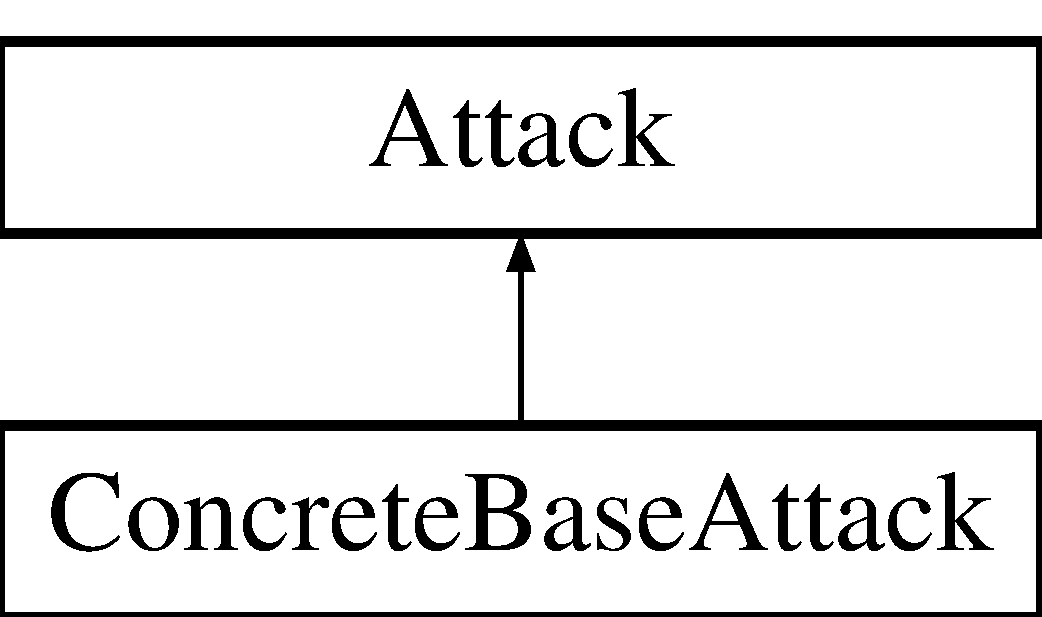
\includegraphics[height=2.000000cm]{classConcreteBaseAttack}
\end{center}
\end{figure}
\subsection*{Fonctions membres publiques}
\begin{DoxyCompactItemize}
\item 
\hypertarget{classConcreteBaseAttack_a1695c43e01c14d65b893443866bc3ca7}{\hyperlink{classConcreteBaseAttack_a1695c43e01c14d65b893443866bc3ca7}{Concrete\+Base\+Attack} (unsigned int ap)}\label{classConcreteBaseAttack_a1695c43e01c14d65b893443866bc3ca7}

\begin{DoxyCompactList}\small\item\em Constructeur. \end{DoxyCompactList}\item 
void \hyperlink{classConcreteBaseAttack_a35cf2248ae6a719ba6041f95ea1428a2}{attack} (\hyperlink{classPosition}{Position} position, \hyperlink{classMap}{Map} $\ast$map, \hyperlink{classUnit}{Unit} $\ast$attacker)
\begin{DoxyCompactList}\small\item\em Méthode d'attaque. \end{DoxyCompactList}\end{DoxyCompactItemize}
\subsection*{Membres hérités additionnels}


\subsection{Description détaillée}
Classe concrete définissant le comportement d'attaque de base des unités normales. 

Définition à la ligne 22 du fichier concrete\+Base\+Attack.\+hpp.



\subsection{Documentation des fonctions membres}
\hypertarget{classConcreteBaseAttack_a35cf2248ae6a719ba6041f95ea1428a2}{\index{Concrete\+Base\+Attack@{Concrete\+Base\+Attack}!attack@{attack}}
\index{attack@{attack}!Concrete\+Base\+Attack@{Concrete\+Base\+Attack}}
\subsubsection[{attack}]{\setlength{\rightskip}{0pt plus 5cm}void Concrete\+Base\+Attack\+::attack (
\begin{DoxyParamCaption}
\item[{{\bf Position}}]{position, }
\item[{{\bf Map} $\ast$}]{map, }
\item[{{\bf Unit} $\ast$}]{attacker}
\end{DoxyParamCaption}
)\hspace{0.3cm}{\ttfamily [virtual]}}}\label{classConcreteBaseAttack_a35cf2248ae6a719ba6041f95ea1428a2}


Méthode d'attaque. 


\begin{DoxyParams}{Paramètres}
{\em position} & une position \\
\hline
{\em map} & une map \\
\hline
{\em attacker} & l'unité qui attaque \\
\hline
\end{DoxyParams}


Implémente \hyperlink{classAttack_aa741caafef0d80bb0a00ce39e5bf6e2d}{Attack}.



La documentation de cette classe a été générée à partir du fichier suivant \+:\begin{DoxyCompactItemize}
\item 
src/\hyperlink{concreteBaseAttack_8hpp}{concrete\+Base\+Attack.\+hpp}\end{DoxyCompactItemize}

\hypertarget{classConcreteBaseAttackSpeBase}{\section{Référence de la classe Concrete\+Base\+Attack\+Spe\+Base}
\label{classConcreteBaseAttackSpeBase}\index{Concrete\+Base\+Attack\+Spe\+Base@{Concrete\+Base\+Attack\+Spe\+Base}}
}
Graphe d'héritage de Concrete\+Base\+Attack\+Spe\+Base\+:\begin{figure}[H]
\begin{center}
\leavevmode
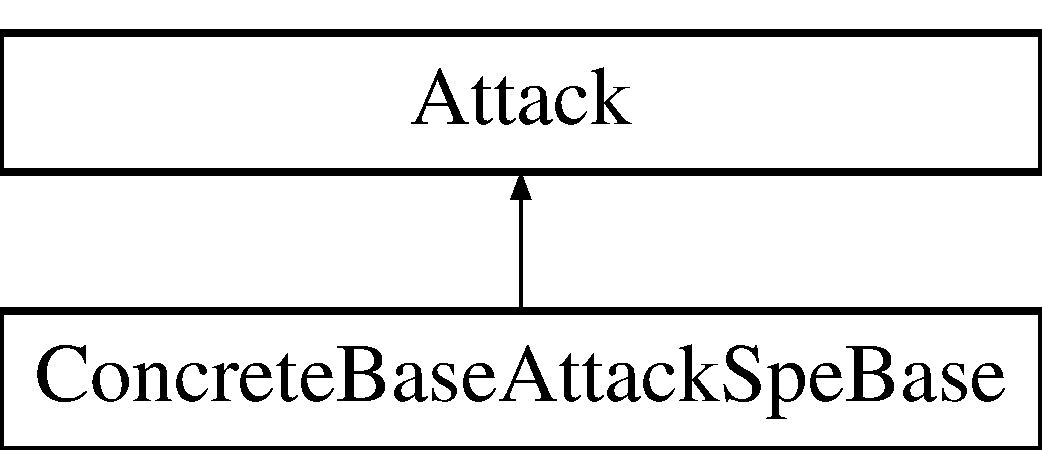
\includegraphics[height=2.000000cm]{classConcreteBaseAttackSpeBase}
\end{center}
\end{figure}
\subsection*{Fonctions membres publiques}
\begin{DoxyCompactItemize}
\item 
\hypertarget{classConcreteBaseAttackSpeBase_a5680fdba17590e8d2cb81be5340206e7}{{\bfseries Concrete\+Base\+Attack\+Spe\+Base} (unsigned int ap)}\label{classConcreteBaseAttackSpeBase_a5680fdba17590e8d2cb81be5340206e7}

\item 
void \hyperlink{classConcreteBaseAttackSpeBase_a4b215e51d3146516ecf77e23d19a92de}{attack} (\hyperlink{classPosition}{Position} position, \hyperlink{classMap}{Map} $\ast$map, \hyperlink{classUnit}{Unit} $\ast$attacker)
\begin{DoxyCompactList}\small\item\em Destructeur (évite les warnings) \end{DoxyCompactList}\end{DoxyCompactItemize}
\subsection*{Membres hérités additionnels}


\subsection{Description détaillée}


Définition à la ligne 21 du fichier concrete\+Base\+Attack\+Spe\+Base.\+hpp.



\subsection{Documentation des fonctions membres}
\hypertarget{classConcreteBaseAttackSpeBase_a4b215e51d3146516ecf77e23d19a92de}{\index{Concrete\+Base\+Attack\+Spe\+Base@{Concrete\+Base\+Attack\+Spe\+Base}!attack@{attack}}
\index{attack@{attack}!Concrete\+Base\+Attack\+Spe\+Base@{Concrete\+Base\+Attack\+Spe\+Base}}
\subsubsection[{attack}]{\setlength{\rightskip}{0pt plus 5cm}void Concrete\+Base\+Attack\+Spe\+Base\+::attack (
\begin{DoxyParamCaption}
\item[{{\bf Position}}]{position, }
\item[{{\bf Map} $\ast$}]{map, }
\item[{{\bf Unit} $\ast$}]{attacker}
\end{DoxyParamCaption}
)\hspace{0.3cm}{\ttfamily [virtual]}}}\label{classConcreteBaseAttackSpeBase_a4b215e51d3146516ecf77e23d19a92de}


Destructeur (évite les warnings) 

Méthode virtuelle pure d'attaque 
\begin{DoxyParams}{Paramètres}
{\em position} & une position \\
\hline
{\em map} & une map \\
\hline
{\em attacker} & l'unité qui attaque \\
\hline
\end{DoxyParams}


Implémente \hyperlink{classAttack_aa741caafef0d80bb0a00ce39e5bf6e2d}{Attack}.



La documentation de cette classe a été générée à partir du fichier suivant \+:\begin{DoxyCompactItemize}
\item 
src/\hyperlink{concreteBaseAttackSpeBase_8hpp}{concrete\+Base\+Attack\+Spe\+Base.\+hpp}\end{DoxyCompactItemize}

\hypertarget{classConcreteConcreteHPLoss}{\section{Référence de la classe Concrete\+Concrete\+H\+P\+Loss}
\label{classConcreteConcreteHPLoss}\index{Concrete\+Concrete\+H\+P\+Loss@{Concrete\+Concrete\+H\+P\+Loss}}
}


Classe concrete définissant le comportement de la perte de point de vie des unités normales.  




{\ttfamily \#include $<$concretehploss.\+hpp$>$}



\subsection{Description détaillée}
Classe concrete définissant le comportement de la perte de point de vie des unités normales. 

Définition à la ligne 14 du fichier concretehploss.\+hpp.



La documentation de cette classe a été générée à partir du fichier suivant \+:\begin{DoxyCompactItemize}
\item 
src/\hyperlink{concretehploss_8hpp}{concretehploss.\+hpp}\end{DoxyCompactItemize}

\hypertarget{classConcreteConcreteHPLossSpeDef}{\section{Référence de la classe Concrete\+Concrete\+H\+P\+Loss\+Spe\+Def}
\label{classConcreteConcreteHPLossSpeDef}\index{Concrete\+Concrete\+H\+P\+Loss\+Spe\+Def@{Concrete\+Concrete\+H\+P\+Loss\+Spe\+Def}}
}


Classe concrete définissant le comportement de la perte de point de vie des unités défensives.  




{\ttfamily \#include $<$concretehplossspedef.\+hpp$>$}



\subsection{Description détaillée}
Classe concrete définissant le comportement de la perte de point de vie des unités défensives. 

Définition à la ligne 14 du fichier concretehplossspedef.\+hpp.



La documentation de cette classe a été générée à partir du fichier suivant \+:\begin{DoxyCompactItemize}
\item 
src/\hyperlink{concretehplossspedef_8hpp}{concretehplossspedef.\+hpp}\end{DoxyCompactItemize}

\hypertarget{classConcreteHPLoss}{\section{Référence de la classe Concrete\+H\+P\+Loss}
\label{classConcreteHPLoss}\index{Concrete\+H\+P\+Loss@{Concrete\+H\+P\+Loss}}
}
Graphe d'héritage de Concrete\+H\+P\+Loss\+:\begin{figure}[H]
\begin{center}
\leavevmode
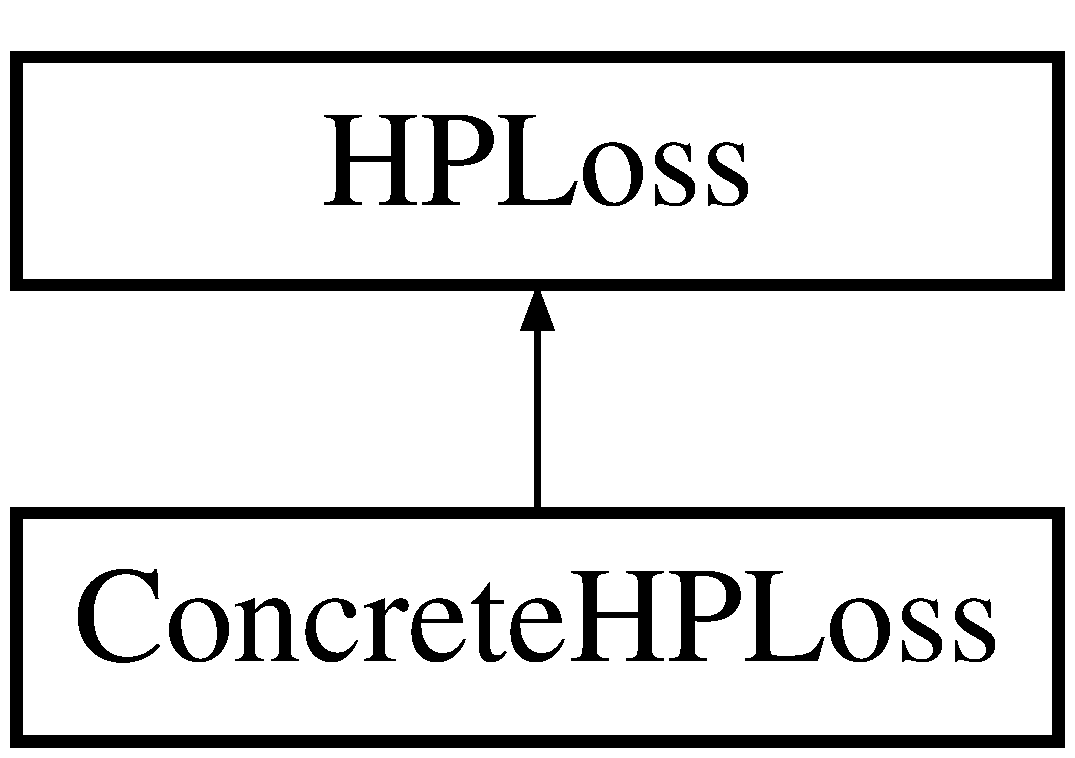
\includegraphics[height=2.000000cm]{classConcreteHPLoss}
\end{center}
\end{figure}
\subsection*{Fonctions membres publiques}
\begin{DoxyCompactItemize}
\item 
void \hyperlink{classConcreteHPLoss_a5bebc84735ab86cd54f19a8488464558}{hp\+Loss} (unsigned int value, \hyperlink{classUnit}{Unit} $\ast$u)
\begin{DoxyCompactList}\small\item\em Perte d'hp des unité \end{DoxyCompactList}\item 
void \hyperlink{classConcreteHPLoss_ae15f6aa597fdc1e1fce3326beb90c335}{hp\+Loss} (unsigned int value, \hyperlink{classBase}{Base} $\ast$b)
\begin{DoxyCompactList}\small\item\em Perte d'hp des bases. \end{DoxyCompactList}\end{DoxyCompactItemize}


\subsection{Description détaillée}


Définition à la ligne 21 du fichier concretehploss.\+hpp.



\subsection{Documentation des fonctions membres}
\hypertarget{classConcreteHPLoss_a5bebc84735ab86cd54f19a8488464558}{\index{Concrete\+H\+P\+Loss@{Concrete\+H\+P\+Loss}!hp\+Loss@{hp\+Loss}}
\index{hp\+Loss@{hp\+Loss}!Concrete\+H\+P\+Loss@{Concrete\+H\+P\+Loss}}
\subsubsection[{hp\+Loss}]{\setlength{\rightskip}{0pt plus 5cm}void Concrete\+H\+P\+Loss\+::hp\+Loss (
\begin{DoxyParamCaption}
\item[{unsigned int}]{value, }
\item[{{\bf Unit} $\ast$}]{u}
\end{DoxyParamCaption}
)\hspace{0.3cm}{\ttfamily [virtual]}}}\label{classConcreteHPLoss_a5bebc84735ab86cd54f19a8488464558}


Perte d'hp des unité 


\begin{DoxyParams}{Paramètres}
{\em value} & un entier positif \\
\hline
{\em u} & l'unité qui prend des dégats \\
\hline
\end{DoxyParams}


Implémente \hyperlink{classHPLoss_a9572e4b06e306798325e2b27d15244e2}{H\+P\+Loss}.

\hypertarget{classConcreteHPLoss_ae15f6aa597fdc1e1fce3326beb90c335}{\index{Concrete\+H\+P\+Loss@{Concrete\+H\+P\+Loss}!hp\+Loss@{hp\+Loss}}
\index{hp\+Loss@{hp\+Loss}!Concrete\+H\+P\+Loss@{Concrete\+H\+P\+Loss}}
\subsubsection[{hp\+Loss}]{\setlength{\rightskip}{0pt plus 5cm}void Concrete\+H\+P\+Loss\+::hp\+Loss (
\begin{DoxyParamCaption}
\item[{unsigned int}]{value, }
\item[{{\bf Base} $\ast$}]{b}
\end{DoxyParamCaption}
)\hspace{0.3cm}{\ttfamily [virtual]}}}\label{classConcreteHPLoss_ae15f6aa597fdc1e1fce3326beb90c335}


Perte d'hp des bases. 


\begin{DoxyParams}{Paramètres}
{\em value} & un entier positif \\
\hline
{\em b} & la base qui prend des dégats \\
\hline
\end{DoxyParams}


Implémente \hyperlink{classHPLoss_a65218bfa1695b56033b5ba894ba0d778}{H\+P\+Loss}.



La documentation de cette classe a été générée à partir du fichier suivant \+:\begin{DoxyCompactItemize}
\item 
src/\hyperlink{concretehploss_8hpp}{concretehploss.\+hpp}\end{DoxyCompactItemize}

\hypertarget{classConcreteHPLossSpeDef}{\section{Référence de la classe Concrete\+H\+P\+Loss\+Spe\+Def}
\label{classConcreteHPLossSpeDef}\index{Concrete\+H\+P\+Loss\+Spe\+Def@{Concrete\+H\+P\+Loss\+Spe\+Def}}
}
Graphe d'héritage de Concrete\+H\+P\+Loss\+Spe\+Def\+:\begin{figure}[H]
\begin{center}
\leavevmode
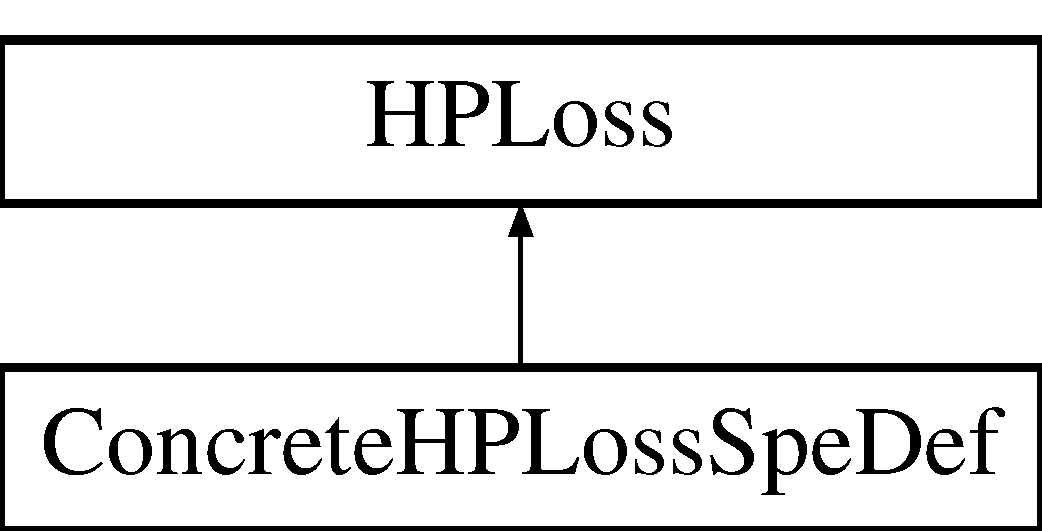
\includegraphics[height=2.000000cm]{classConcreteHPLossSpeDef}
\end{center}
\end{figure}
\subsection*{Fonctions membres publiques}
\begin{DoxyCompactItemize}
\item 
void \hyperlink{classConcreteHPLossSpeDef_ad62272f839de14217c84688bd2fa5aba}{hp\+Loss} (unsigned int value, \hyperlink{classUnit}{Unit} $\ast$u)
\begin{DoxyCompactList}\small\item\em Perte d'hp des unité \end{DoxyCompactList}\item 
void \hyperlink{classConcreteHPLossSpeDef_ad7b1e1fa122742674fe53e89a6c4b261}{hp\+Loss} (unsigned int value, \hyperlink{classBase}{Base} $\ast$b)
\begin{DoxyCompactList}\small\item\em Perte d'hp des bases. \end{DoxyCompactList}\end{DoxyCompactItemize}


\subsection{Description détaillée}


Définition à la ligne 21 du fichier concretehplossspedef.\+hpp.



\subsection{Documentation des fonctions membres}
\hypertarget{classConcreteHPLossSpeDef_ad62272f839de14217c84688bd2fa5aba}{\index{Concrete\+H\+P\+Loss\+Spe\+Def@{Concrete\+H\+P\+Loss\+Spe\+Def}!hp\+Loss@{hp\+Loss}}
\index{hp\+Loss@{hp\+Loss}!Concrete\+H\+P\+Loss\+Spe\+Def@{Concrete\+H\+P\+Loss\+Spe\+Def}}
\subsubsection[{hp\+Loss}]{\setlength{\rightskip}{0pt plus 5cm}void Concrete\+H\+P\+Loss\+Spe\+Def\+::hp\+Loss (
\begin{DoxyParamCaption}
\item[{unsigned int}]{value, }
\item[{{\bf Unit} $\ast$}]{u}
\end{DoxyParamCaption}
)\hspace{0.3cm}{\ttfamily [virtual]}}}\label{classConcreteHPLossSpeDef_ad62272f839de14217c84688bd2fa5aba}


Perte d'hp des unité 


\begin{DoxyParams}{Paramètres}
{\em value} & un entier positif \\
\hline
{\em u} & l'unité qui prend des dégats \\
\hline
\end{DoxyParams}


Implémente \hyperlink{classHPLoss_a9572e4b06e306798325e2b27d15244e2}{H\+P\+Loss}.

\hypertarget{classConcreteHPLossSpeDef_ad7b1e1fa122742674fe53e89a6c4b261}{\index{Concrete\+H\+P\+Loss\+Spe\+Def@{Concrete\+H\+P\+Loss\+Spe\+Def}!hp\+Loss@{hp\+Loss}}
\index{hp\+Loss@{hp\+Loss}!Concrete\+H\+P\+Loss\+Spe\+Def@{Concrete\+H\+P\+Loss\+Spe\+Def}}
\subsubsection[{hp\+Loss}]{\setlength{\rightskip}{0pt plus 5cm}void Concrete\+H\+P\+Loss\+Spe\+Def\+::hp\+Loss (
\begin{DoxyParamCaption}
\item[{unsigned int}]{value, }
\item[{{\bf Base} $\ast$}]{b}
\end{DoxyParamCaption}
)\hspace{0.3cm}{\ttfamily [virtual]}}}\label{classConcreteHPLossSpeDef_ad7b1e1fa122742674fe53e89a6c4b261}


Perte d'hp des bases. 


\begin{DoxyParams}{Paramètres}
{\em value} & un entier positif \\
\hline
{\em b} & la base qui prend des dégats \\
\hline
\end{DoxyParams}


Implémente \hyperlink{classHPLoss_a65218bfa1695b56033b5ba894ba0d778}{H\+P\+Loss}.



La documentation de cette classe a été générée à partir du fichier suivant \+:\begin{DoxyCompactItemize}
\item 
src/\hyperlink{concretehplossspedef_8hpp}{concretehplossspedef.\+hpp}\end{DoxyCompactItemize}

\hypertarget{classConcreteMove}{\section{Référence de la classe Concrete\+Move}
\label{classConcreteMove}\index{Concrete\+Move@{Concrete\+Move}}
}


Classe concrete définissant le comportement de déplacement des unités mouvantes.  


Graphe d'héritage de Concrete\+Move\+:\begin{figure}[H]
\begin{center}
\leavevmode
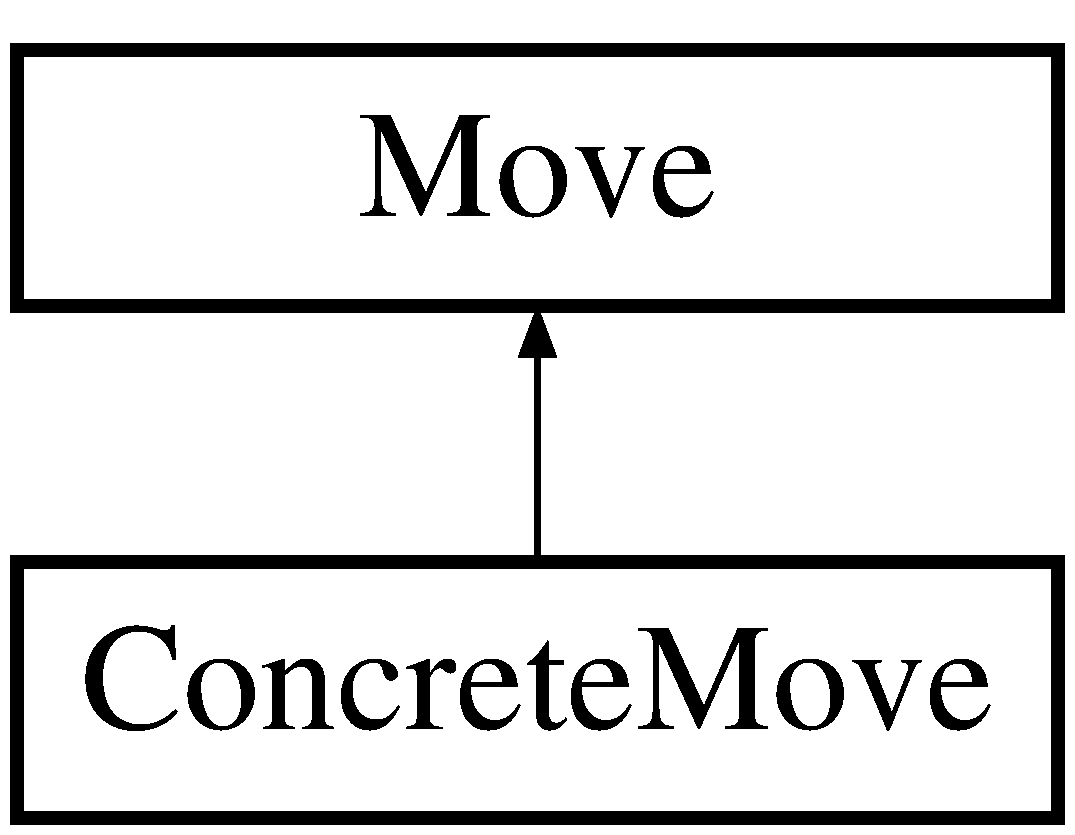
\includegraphics[height=2.000000cm]{classConcreteMove}
\end{center}
\end{figure}
\subsection*{Fonctions membres publiques}
\begin{DoxyCompactItemize}
\item 
void \hyperlink{classConcreteMove_adbbcf93faa6dad1660a922618b905ff1}{move} (\hyperlink{classPath}{Path} $\ast$path, \hyperlink{classMap}{Map} $\ast$map, \hyperlink{classUnit}{Unit} $\ast$u)
\begin{DoxyCompactList}\small\item\em déplacement d'une unité \end{DoxyCompactList}\end{DoxyCompactItemize}


\subsection{Description détaillée}
Classe concrete définissant le comportement de déplacement des unités mouvantes. 

Définition à la ligne 22 du fichier concretemove.\+hpp.



\subsection{Documentation des fonctions membres}
\hypertarget{classConcreteMove_adbbcf93faa6dad1660a922618b905ff1}{\index{Concrete\+Move@{Concrete\+Move}!move@{move}}
\index{move@{move}!Concrete\+Move@{Concrete\+Move}}
\subsubsection[{move}]{\setlength{\rightskip}{0pt plus 5cm}void Concrete\+Move\+::move (
\begin{DoxyParamCaption}
\item[{{\bf Path} $\ast$}]{path, }
\item[{{\bf Map} $\ast$}]{map, }
\item[{{\bf Unit} $\ast$}]{u}
\end{DoxyParamCaption}
)\hspace{0.3cm}{\ttfamily [virtual]}}}\label{classConcreteMove_adbbcf93faa6dad1660a922618b905ff1}


déplacement d'une unité 


\begin{DoxyParams}{Paramètres}
{\em path} & un chemin \\
\hline
{\em map} & une map \\
\hline
{\em u} & une unité \\
\hline
\end{DoxyParams}


Implémente \hyperlink{classMove_ace4540308f0bbd21d71a18b2ff7c972d}{Move}.



La documentation de cette classe a été générée à partir du fichier suivant \+:\begin{DoxyCompactItemize}
\item 
src/\hyperlink{concretemove_8hpp}{concretemove.\+hpp}\end{DoxyCompactItemize}

\hypertarget{classData}{\section{Référence de la classe Data}
\label{classData}\index{Data@{Data}}
}


Classe qui centralise toute les données du jeu.  




{\ttfamily \#include $<$data.\+hpp$>$}

\subsection*{Fonctions membres publiques}
\begin{DoxyCompactItemize}
\item 
\hypertarget{classData_af11f741cb7f587e2e495452a8905a22a}{\hyperlink{classData_af11f741cb7f587e2e495452a8905a22a}{Data} ()}\label{classData_af11f741cb7f587e2e495452a8905a22a}

\begin{DoxyCompactList}\small\item\em Constructeur. \end{DoxyCompactList}\item 
\hypertarget{classData_aab31956423290f0d62dcca47ab4d16dd}{\hyperlink{classData_aab31956423290f0d62dcca47ab4d16dd}{$\sim$\+Data} ()}\label{classData_aab31956423290f0d62dcca47ab4d16dd}

\begin{DoxyCompactList}\small\item\em Destructeur. \end{DoxyCompactList}\item 
std\+::vector$<$ std\+::vector\\*
$<$ unsigned int $>$ $>$ \hyperlink{classData_afa20d9cff2f1a3e174b7afcfb5a324fe}{get\+Tiles\+\_\+\+Map} ()
\item 
std\+::vector$<$ \hyperlink{classPosition}{Position} $>$ \hyperlink{classData_a37701a5ef2e31ae2b0c7a78ac943e316}{get\+Starting\+Positions\+\_\+\+Map} ()
\item 
std\+::map$<$ std\+::string, \\*
unsigned int $>$ \hyperlink{classData_a28356240fd39ccba1e700b903c4bec95}{get\+Unsigned\+Int\+Data\+\_\+\+Base} ()
\item 
\hyperlink{classHPLoss}{H\+P\+Loss} $\ast$ \hyperlink{classData_ac3ee5887346af353d837b0cd989e86df}{get\+H\+P\+Loss\+Behavior\+\_\+\+Base} ()
\item 
\hyperlink{classSpawner}{Spawner} $\ast$ \hyperlink{classData_ae1e9282b13a0c50cd3e25da0de4527ac}{get\+Spawner} (std\+::string classe)
\item 
bool \hyperlink{classData_ad3fadb201a8698fee0981d7567024b23}{is\+Classe} (std\+::string classe)
\item 
std\+::vector$<$ std\+::string $>$ \hyperlink{classData_a6da2bc0e5b92dd41c3e3cae7440c2a1d}{get\+Classes} ()
\item 
unsigned int \hyperlink{classData_a24b4103d5c16ef50f996e2e058ee41e2}{get\+Golds\+\_\+\+Player} ()
\end{DoxyCompactItemize}


\subsection{Description détaillée}
Classe qui centralise toute les données du jeu. 

Définition à la ligne 30 du fichier data.\+hpp.



\subsection{Documentation des fonctions membres}
\hypertarget{classData_a6da2bc0e5b92dd41c3e3cae7440c2a1d}{\index{Data@{Data}!get\+Classes@{get\+Classes}}
\index{get\+Classes@{get\+Classes}!Data@{Data}}
\subsubsection[{get\+Classes}]{\setlength{\rightskip}{0pt plus 5cm}std\+::vector$<$std\+::string$>$ Data\+::get\+Classes (
\begin{DoxyParamCaption}
{}
\end{DoxyParamCaption}
)}}\label{classData_a6da2bc0e5b92dd41c3e3cae7440c2a1d}
Accesseur de la liste des classes \begin{DoxyReturn}{Renvoie}
un tableau de string 
\end{DoxyReturn}
\hypertarget{classData_a24b4103d5c16ef50f996e2e058ee41e2}{\index{Data@{Data}!get\+Golds\+\_\+\+Player@{get\+Golds\+\_\+\+Player}}
\index{get\+Golds\+\_\+\+Player@{get\+Golds\+\_\+\+Player}!Data@{Data}}
\subsubsection[{get\+Golds\+\_\+\+Player}]{\setlength{\rightskip}{0pt plus 5cm}unsigned int Data\+::get\+Golds\+\_\+\+Player (
\begin{DoxyParamCaption}
{}
\end{DoxyParamCaption}
)}}\label{classData_a24b4103d5c16ef50f996e2e058ee41e2}
Retourne le nombre de golds des joueurs à l'initialisattion \begin{DoxyReturn}{Renvoie}
un unsigned int 
\end{DoxyReturn}
\hypertarget{classData_ac3ee5887346af353d837b0cd989e86df}{\index{Data@{Data}!get\+H\+P\+Loss\+Behavior\+\_\+\+Base@{get\+H\+P\+Loss\+Behavior\+\_\+\+Base}}
\index{get\+H\+P\+Loss\+Behavior\+\_\+\+Base@{get\+H\+P\+Loss\+Behavior\+\_\+\+Base}!Data@{Data}}
\subsubsection[{get\+H\+P\+Loss\+Behavior\+\_\+\+Base}]{\setlength{\rightskip}{0pt plus 5cm}{\bf H\+P\+Loss}$\ast$ Data\+::get\+H\+P\+Loss\+Behavior\+\_\+\+Base (
\begin{DoxyParamCaption}
{}
\end{DoxyParamCaption}
)}}\label{classData_ac3ee5887346af353d837b0cd989e86df}
Retourne le comportement de perte d'hp des bases \hypertarget{classData_ae1e9282b13a0c50cd3e25da0de4527ac}{\index{Data@{Data}!get\+Spawner@{get\+Spawner}}
\index{get\+Spawner@{get\+Spawner}!Data@{Data}}
\subsubsection[{get\+Spawner}]{\setlength{\rightskip}{0pt plus 5cm}{\bf Spawner}$\ast$ Data\+::get\+Spawner (
\begin{DoxyParamCaption}
\item[{std\+::string}]{classe}
\end{DoxyParamCaption}
)}}\label{classData_ae1e9282b13a0c50cd3e25da0de4527ac}
Retourne le spawner associé à la classe en paramètre 
\begin{DoxyParams}{Paramètres}
{\em classe} & la classe dont on veut le spawner \\
\hline
\end{DoxyParams}
\begin{DoxyReturn}{Renvoie}
un pointeur vers spawner 
\end{DoxyReturn}
\hypertarget{classData_a37701a5ef2e31ae2b0c7a78ac943e316}{\index{Data@{Data}!get\+Starting\+Positions\+\_\+\+Map@{get\+Starting\+Positions\+\_\+\+Map}}
\index{get\+Starting\+Positions\+\_\+\+Map@{get\+Starting\+Positions\+\_\+\+Map}!Data@{Data}}
\subsubsection[{get\+Starting\+Positions\+\_\+\+Map}]{\setlength{\rightskip}{0pt plus 5cm}std\+::vector$<${\bf Position}$>$ Data\+::get\+Starting\+Positions\+\_\+\+Map (
\begin{DoxyParamCaption}
{}
\end{DoxyParamCaption}
)}}\label{classData_a37701a5ef2e31ae2b0c7a78ac943e316}
Retourne un vector contenant les positions de départ de la map \begin{DoxyReturn}{Renvoie}
un tableau de position 
\end{DoxyReturn}
\hypertarget{classData_afa20d9cff2f1a3e174b7afcfb5a324fe}{\index{Data@{Data}!get\+Tiles\+\_\+\+Map@{get\+Tiles\+\_\+\+Map}}
\index{get\+Tiles\+\_\+\+Map@{get\+Tiles\+\_\+\+Map}!Data@{Data}}
\subsubsection[{get\+Tiles\+\_\+\+Map}]{\setlength{\rightskip}{0pt plus 5cm}std\+::vector$<$std\+::vector$<$unsigned int$>$ $>$ Data\+::get\+Tiles\+\_\+\+Map (
\begin{DoxyParamCaption}
{}
\end{DoxyParamCaption}
)}}\label{classData_afa20d9cff2f1a3e174b7afcfb5a324fe}
Méthode qui retourne un vector de vector qui correspond aux cases accessibles ou non de la map de base sans les décors \begin{DoxyReturn}{Renvoie}
un tableau de tableau de booleen 
\end{DoxyReturn}
\hypertarget{classData_a28356240fd39ccba1e700b903c4bec95}{\index{Data@{Data}!get\+Unsigned\+Int\+Data\+\_\+\+Base@{get\+Unsigned\+Int\+Data\+\_\+\+Base}}
\index{get\+Unsigned\+Int\+Data\+\_\+\+Base@{get\+Unsigned\+Int\+Data\+\_\+\+Base}!Data@{Data}}
\subsubsection[{get\+Unsigned\+Int\+Data\+\_\+\+Base}]{\setlength{\rightskip}{0pt plus 5cm}std\+::map$<$std\+::string, unsigned int$>$ Data\+::get\+Unsigned\+Int\+Data\+\_\+\+Base (
\begin{DoxyParamCaption}
{}
\end{DoxyParamCaption}
)}}\label{classData_a28356240fd39ccba1e700b903c4bec95}
Retourne toutes les données de type unsigned int de la classe base afin d'initialiser les instances de celle-\/ci \begin{DoxyReturn}{Renvoie}
une map string-\/$>$unsigned int 
\end{DoxyReturn}
\hypertarget{classData_ad3fadb201a8698fee0981d7567024b23}{\index{Data@{Data}!is\+Classe@{is\+Classe}}
\index{is\+Classe@{is\+Classe}!Data@{Data}}
\subsubsection[{is\+Classe}]{\setlength{\rightskip}{0pt plus 5cm}bool Data\+::is\+Classe (
\begin{DoxyParamCaption}
\item[{std\+::string}]{classe}
\end{DoxyParamCaption}
)}}\label{classData_ad3fadb201a8698fee0981d7567024b23}
Méthode qui vérifie si une classe existe 
\begin{DoxyParams}{Paramètres}
{\em classe} & la classe dont on veut savoir si elle existe \\
\hline
\end{DoxyParams}
\begin{DoxyReturn}{Renvoie}
vrai si la classe est clé de la map \+\_\+spawner\+List 
\end{DoxyReturn}


La documentation de cette classe a été générée à partir du fichier suivant \+:\begin{DoxyCompactItemize}
\item 
src/\hyperlink{data_8hpp}{data.\+hpp}\end{DoxyCompactItemize}

\hypertarget{classGame}{\section{Référence de la classe Game}
\label{classGame}\index{Game@{Game}}
}


Classe qui centralisera tout le jeu.  




{\ttfamily \#include $<$game.\+hpp$>$}

Graphe d'héritage de Game\+:\begin{figure}[H]
\begin{center}
\leavevmode
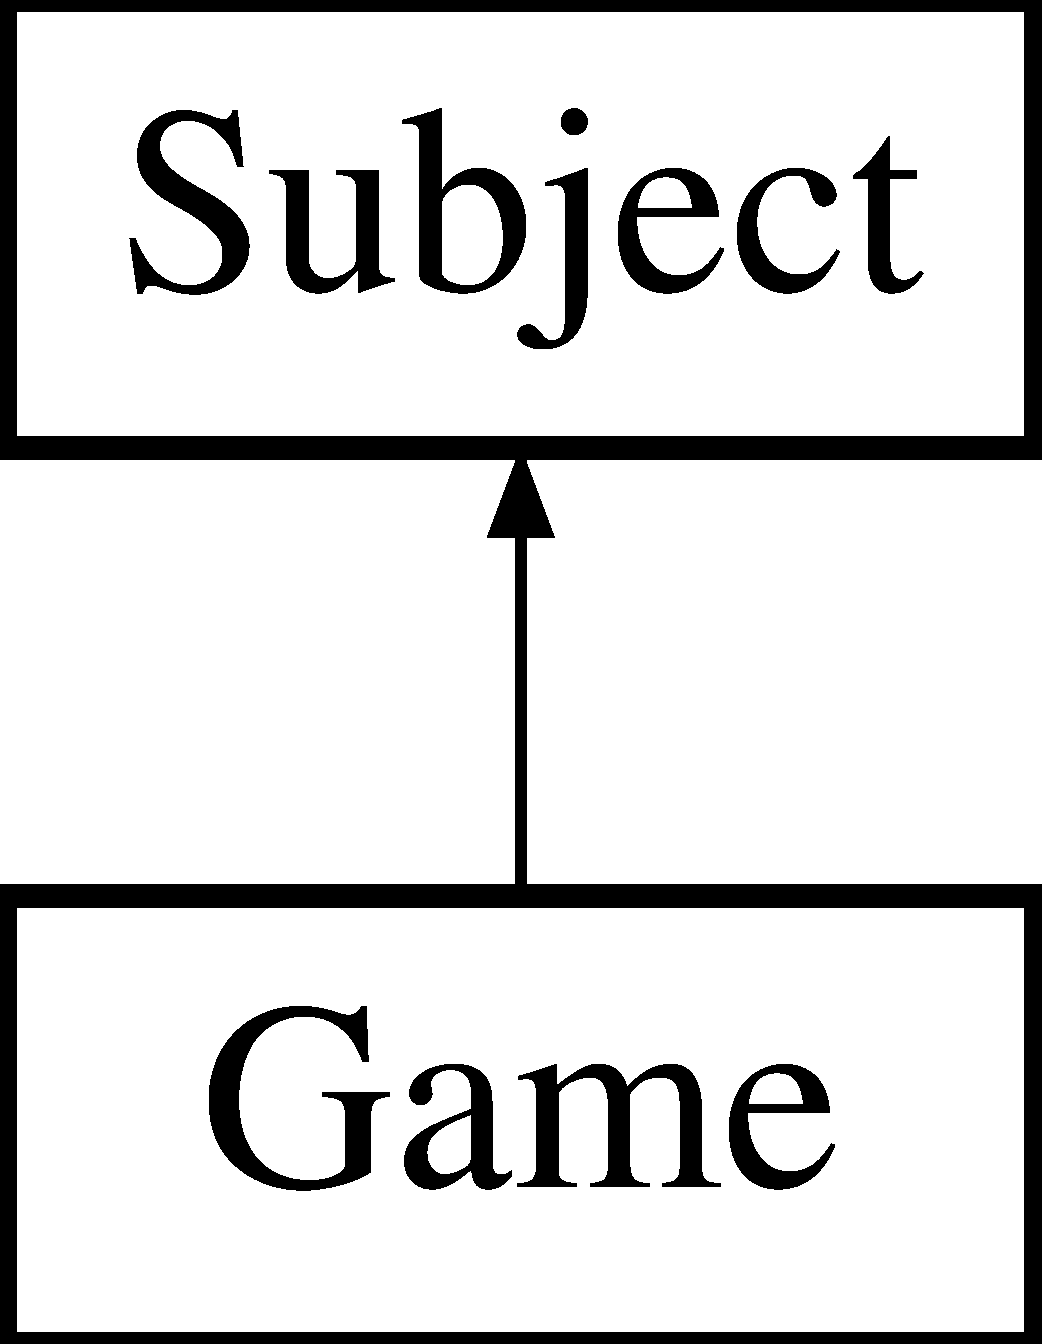
\includegraphics[height=2.000000cm]{classGame}
\end{center}
\end{figure}
\subsection*{Fonctions membres publiques}
\begin{DoxyCompactItemize}
\item 
\hypertarget{classGame_ad59df6562a58a614fda24622d3715b65}{\hyperlink{classGame_ad59df6562a58a614fda24622d3715b65}{Game} ()}\label{classGame_ad59df6562a58a614fda24622d3715b65}

\begin{DoxyCompactList}\small\item\em constructeur \end{DoxyCompactList}\item 
\hypertarget{classGame_ae3d112ca6e0e55150d2fdbc704474530}{\hyperlink{classGame_ae3d112ca6e0e55150d2fdbc704474530}{$\sim$\+Game} ()}\label{classGame_ae3d112ca6e0e55150d2fdbc704474530}

\begin{DoxyCompactList}\small\item\em destructeur \end{DoxyCompactList}\item 
\hypertarget{classGame_aa333825d0bca80e91e53c7e23f053405}{void \hyperlink{classGame_aa333825d0bca80e91e53c7e23f053405}{play} ()}\label{classGame_aa333825d0bca80e91e53c7e23f053405}

\begin{DoxyCompactList}\small\item\em Boucle du jeu, fini lorsque la commande tapée est /quit. \end{DoxyCompactList}\item 
\hypertarget{classGame_a987b5442cddbc9376b7fe55a9fcbd42e}{void \hyperlink{classGame_a987b5442cddbc9376b7fe55a9fcbd42e}{end\+Turn} ()}\label{classGame_a987b5442cddbc9376b7fe55a9fcbd42e}

\begin{DoxyCompactList}\small\item\em Méthode centralisant toutes les actions à effectuer à la fin du tour. \end{DoxyCompactList}\item 
\hypertarget{classGame_a217c5bd3b04bcf146b312cb17e2621e3}{bool \hyperlink{classGame_a217c5bd3b04bcf146b312cb17e2621e3}{end\+Of\+Game} ()}\label{classGame_a217c5bd3b04bcf146b312cb17e2621e3}

\begin{DoxyCompactList}\small\item\em Méthode qui vérifie si un des joueurs à gagné \end{DoxyCompactList}\item 
\hypertarget{classGame_a2f6be379e2d5bc1cce58f1ec96422ba8}{void \hyperlink{classGame_a2f6be379e2d5bc1cce58f1ec96422ba8}{help\+Command} ()}\label{classGame_a2f6be379e2d5bc1cce58f1ec96422ba8}

\begin{DoxyCompactList}\small\item\em Actions lors de la détection de /help. \end{DoxyCompactList}\item 
\hypertarget{classGame_a2be014c3f87a1a6f9169ee0c3d002360}{void \hyperlink{classGame_a2be014c3f87a1a6f9169ee0c3d002360}{quit\+Command} ()}\label{classGame_a2be014c3f87a1a6f9169ee0c3d002360}

\begin{DoxyCompactList}\small\item\em Actions lors de la détection de /quit. \end{DoxyCompactList}\item 
\hypertarget{classGame_a762c24a729cfdc357acbd5c6ecc4c4f8}{void \hyperlink{classGame_a762c24a729cfdc357acbd5c6ecc4c4f8}{summon\+Command} (std\+::vector$<$ std\+::string $>$ command)}\label{classGame_a762c24a729cfdc357acbd5c6ecc4c4f8}

\begin{DoxyCompactList}\small\item\em Actions lors de la détection de /summon. \end{DoxyCompactList}\item 
\hypertarget{classGame_af22614489ceb0cf9a0081016314c75df}{void \hyperlink{classGame_af22614489ceb0cf9a0081016314c75df}{units\+Command} ()}\label{classGame_af22614489ceb0cf9a0081016314c75df}

\begin{DoxyCompactList}\small\item\em Actions lors de la détection de /units. \end{DoxyCompactList}\item 
\hypertarget{classGame_a470d2a7a0da91c8287276d6135840dfd}{void \hyperlink{classGame_a470d2a7a0da91c8287276d6135840dfd}{golds\+Command} ()}\label{classGame_a470d2a7a0da91c8287276d6135840dfd}

\begin{DoxyCompactList}\small\item\em Actions lors de la détection de /golds. \end{DoxyCompactList}\item 
\hypertarget{classGame_acea1269edf0a00ada8e765e385ab5df1}{void \hyperlink{classGame_acea1269edf0a00ada8e765e385ab5df1}{infos\+Command} (std\+::vector$<$ std\+::string $>$ command)}\label{classGame_acea1269edf0a00ada8e765e385ab5df1}

\begin{DoxyCompactList}\small\item\em Actions lors de la détection de /infos. \end{DoxyCompactList}\item 
\hypertarget{classGame_a3b1e53d7df15b62d651830bbd47a7516}{void \hyperlink{classGame_a3b1e53d7df15b62d651830bbd47a7516}{move\+Command} (std\+::vector$<$ std\+::string $>$ command)}\label{classGame_a3b1e53d7df15b62d651830bbd47a7516}

\begin{DoxyCompactList}\small\item\em Actions lors de la détection de /move. \end{DoxyCompactList}\item 
\hypertarget{classGame_a27e73a42585e02a6c375413f803b0032}{void \hyperlink{classGame_a27e73a42585e02a6c375413f803b0032}{attack\+Command} (std\+::vector$<$ std\+::string $>$ command)}\label{classGame_a27e73a42585e02a6c375413f803b0032}

\begin{DoxyCompactList}\small\item\em Actions lors de la détection de /attack. \end{DoxyCompactList}\item 
void \hyperlink{classGame_a7c81b1033a3a8d6758ab0bf1c10a451c}{add\+Obs} (\hyperlink{classObserver}{Observer} $\ast$o)
\begin{DoxyCompactList}\small\item\em Ajout d'un poiteur vers observateur à la liste obs. \end{DoxyCompactList}\item 
void \hyperlink{classGame_a759618d920dd0e0f74f4bba89d35e56e}{rm\+Obs} (\hyperlink{classObserver}{Observer} $\ast$o)
\begin{DoxyCompactList}\small\item\em La suppression d'un pointeur vers observateur de la liste obs, s'il existe. \end{DoxyCompactList}\item 
\hypertarget{classGame_a3ac1bb304b96d6df0d350d39dc651cd2}{void \hyperlink{classGame_a3ac1bb304b96d6df0d350d39dc651cd2}{notify\+Obs} ()}\label{classGame_a3ac1bb304b96d6df0d350d39dc651cd2}

\begin{DoxyCompactList}\small\item\em Notifie à tous les observateurs de la liste obs que cette classe a changé \end{DoxyCompactList}\item 
\hypertarget{classGame_af36ccea6518e85542e7efc07ba425de0}{\hyperlink{classData}{Data} $\ast$ \hyperlink{classGame_af36ccea6518e85542e7efc07ba425de0}{get\+Data} ()}\label{classGame_af36ccea6518e85542e7efc07ba425de0}

\begin{DoxyCompactList}\small\item\em Retourne les data pour l'observer \hyperlink{classWindow}{Window}. \end{DoxyCompactList}\item 
\hypertarget{classGame_af2a02d3d8e78f4246c97ae06dd74f04f}{\hyperlink{classMap}{Map} $\ast$ \hyperlink{classGame_af2a02d3d8e78f4246c97ae06dd74f04f}{get\+Map} ()}\label{classGame_af2a02d3d8e78f4246c97ae06dd74f04f}

\begin{DoxyCompactList}\small\item\em Retourne la map pour l'observer \hyperlink{classWindow}{Window}. \end{DoxyCompactList}\end{DoxyCompactItemize}


\subsection{Description détaillée}
Classe qui centralisera tout le jeu. 

Définition à la ligne 29 du fichier game.\+hpp.



\subsection{Documentation des fonctions membres}
\hypertarget{classGame_a7c81b1033a3a8d6758ab0bf1c10a451c}{\index{Game@{Game}!add\+Obs@{add\+Obs}}
\index{add\+Obs@{add\+Obs}!Game@{Game}}
\subsubsection[{add\+Obs}]{\setlength{\rightskip}{0pt plus 5cm}void Game\+::add\+Obs (
\begin{DoxyParamCaption}
\item[{{\bf Observer} $\ast$}]{o}
\end{DoxyParamCaption}
)\hspace{0.3cm}{\ttfamily [virtual]}}}\label{classGame_a7c81b1033a3a8d6758ab0bf1c10a451c}


Ajout d'un poiteur vers observateur à la liste obs. 


\begin{DoxyParams}{Paramètres}
{\em o} & un pointeur vers observateur \\
\hline
\end{DoxyParams}


Implémente \hyperlink{classSubject_a4a12fdee2e95909a575066103986fa85}{Subject}.

\hypertarget{classGame_a759618d920dd0e0f74f4bba89d35e56e}{\index{Game@{Game}!rm\+Obs@{rm\+Obs}}
\index{rm\+Obs@{rm\+Obs}!Game@{Game}}
\subsubsection[{rm\+Obs}]{\setlength{\rightskip}{0pt plus 5cm}void Game\+::rm\+Obs (
\begin{DoxyParamCaption}
\item[{{\bf Observer} $\ast$}]{o}
\end{DoxyParamCaption}
)\hspace{0.3cm}{\ttfamily [virtual]}}}\label{classGame_a759618d920dd0e0f74f4bba89d35e56e}


La suppression d'un pointeur vers observateur de la liste obs, s'il existe. 


\begin{DoxyParams}{Paramètres}
{\em o} & un pointeur vers observateur \\
\hline
\end{DoxyParams}


Implémente \hyperlink{classSubject_a1005f6c36e1a65fb13f1f0fa908b82e0}{Subject}.



La documentation de cette classe a été générée à partir du fichier suivant \+:\begin{DoxyCompactItemize}
\item 
src/\hyperlink{game_8hpp}{game.\+hpp}\end{DoxyCompactItemize}

\hypertarget{classHPLoss}{\section{Référence de la classe H\+P\+Loss}
\label{classHPLoss}\index{H\+P\+Loss@{H\+P\+Loss}}
}


Classe virtuelle pure permettant l'utilisation de différents comportement de la perte de points de vie selon l'unité. Elle est utilisée dans le cadre du pattern Strategy.  




{\ttfamily \#include $<$hploss.\+hpp$>$}

Graphe d'héritage de H\+P\+Loss\+:\begin{figure}[H]
\begin{center}
\leavevmode
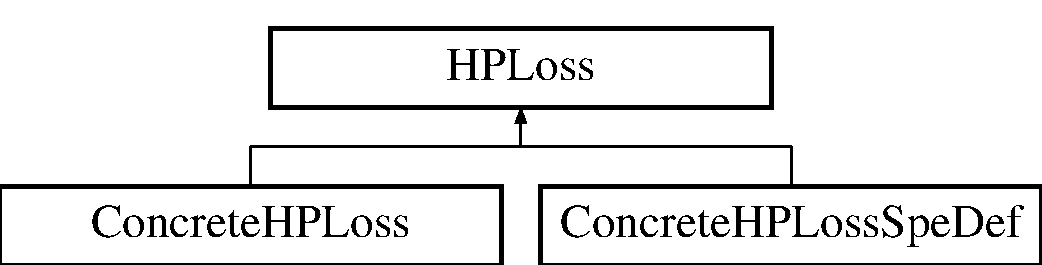
\includegraphics[height=2.000000cm]{classHPLoss}
\end{center}
\end{figure}
\subsection*{Fonctions membres publiques}
\begin{DoxyCompactItemize}
\item 
virtual void \hyperlink{classHPLoss_a9572e4b06e306798325e2b27d15244e2}{hp\+Loss} (unsigned int value, \hyperlink{classUnit}{Unit} $\ast$u)=0
\begin{DoxyCompactList}\small\item\em destructeur (évite les warning) \end{DoxyCompactList}\item 
virtual void \hyperlink{classHPLoss_a65218bfa1695b56033b5ba894ba0d778}{hp\+Loss} (unsigned int value, \hyperlink{classBase}{Base} $\ast$b)=0
\begin{DoxyCompactList}\small\item\em Méthode virtuelle pure de perte d'hp des bases. \end{DoxyCompactList}\end{DoxyCompactItemize}


\subsection{Description détaillée}
Classe virtuelle pure permettant l'utilisation de différents comportement de la perte de points de vie selon l'unité. Elle est utilisée dans le cadre du pattern Strategy. 

Définition à la ligne 20 du fichier hploss.\+hpp.



\subsection{Documentation des fonctions membres}
\hypertarget{classHPLoss_a9572e4b06e306798325e2b27d15244e2}{\index{H\+P\+Loss@{H\+P\+Loss}!hp\+Loss@{hp\+Loss}}
\index{hp\+Loss@{hp\+Loss}!H\+P\+Loss@{H\+P\+Loss}}
\subsubsection[{hp\+Loss}]{\setlength{\rightskip}{0pt plus 5cm}virtual void H\+P\+Loss\+::hp\+Loss (
\begin{DoxyParamCaption}
\item[{unsigned int}]{value, }
\item[{{\bf Unit} $\ast$}]{u}
\end{DoxyParamCaption}
)\hspace{0.3cm}{\ttfamily [pure virtual]}}}\label{classHPLoss_a9572e4b06e306798325e2b27d15244e2}


destructeur (évite les warning) 

Méthode virtuelle pure de perte d'hp des unité 
\begin{DoxyParams}{Paramètres}
{\em value} & un entier positif \\
\hline
{\em u} & l'unité qui prend des dégats \\
\hline
\end{DoxyParams}


Implémenté dans \hyperlink{classConcreteHPLoss_a5bebc84735ab86cd54f19a8488464558}{Concrete\+H\+P\+Loss}, et \hyperlink{classConcreteHPLossSpeDef_ad62272f839de14217c84688bd2fa5aba}{Concrete\+H\+P\+Loss\+Spe\+Def}.

\hypertarget{classHPLoss_a65218bfa1695b56033b5ba894ba0d778}{\index{H\+P\+Loss@{H\+P\+Loss}!hp\+Loss@{hp\+Loss}}
\index{hp\+Loss@{hp\+Loss}!H\+P\+Loss@{H\+P\+Loss}}
\subsubsection[{hp\+Loss}]{\setlength{\rightskip}{0pt plus 5cm}virtual void H\+P\+Loss\+::hp\+Loss (
\begin{DoxyParamCaption}
\item[{unsigned int}]{value, }
\item[{{\bf Base} $\ast$}]{b}
\end{DoxyParamCaption}
)\hspace{0.3cm}{\ttfamily [pure virtual]}}}\label{classHPLoss_a65218bfa1695b56033b5ba894ba0d778}


Méthode virtuelle pure de perte d'hp des bases. 


\begin{DoxyParams}{Paramètres}
{\em value} & un entier positif \\
\hline
{\em b} & la base qui prend des dégats \\
\hline
\end{DoxyParams}


Implémenté dans \hyperlink{classConcreteHPLoss_ae15f6aa597fdc1e1fce3326beb90c335}{Concrete\+H\+P\+Loss}, et \hyperlink{classConcreteHPLossSpeDef_ad7b1e1fa122742674fe53e89a6c4b261}{Concrete\+H\+P\+Loss\+Spe\+Def}.



La documentation de cette classe a été générée à partir du fichier suivant \+:\begin{DoxyCompactItemize}
\item 
src/\hyperlink{hploss_8hpp}{hploss.\+hpp}\end{DoxyCompactItemize}

\hypertarget{classKnight}{\section{Référence de la classe Knight}
\label{classKnight}\index{Knight@{Knight}}
}


Classe définissant un chevalier.  


Graphe d'héritage de Knight\+:\begin{figure}[H]
\begin{center}
\leavevmode
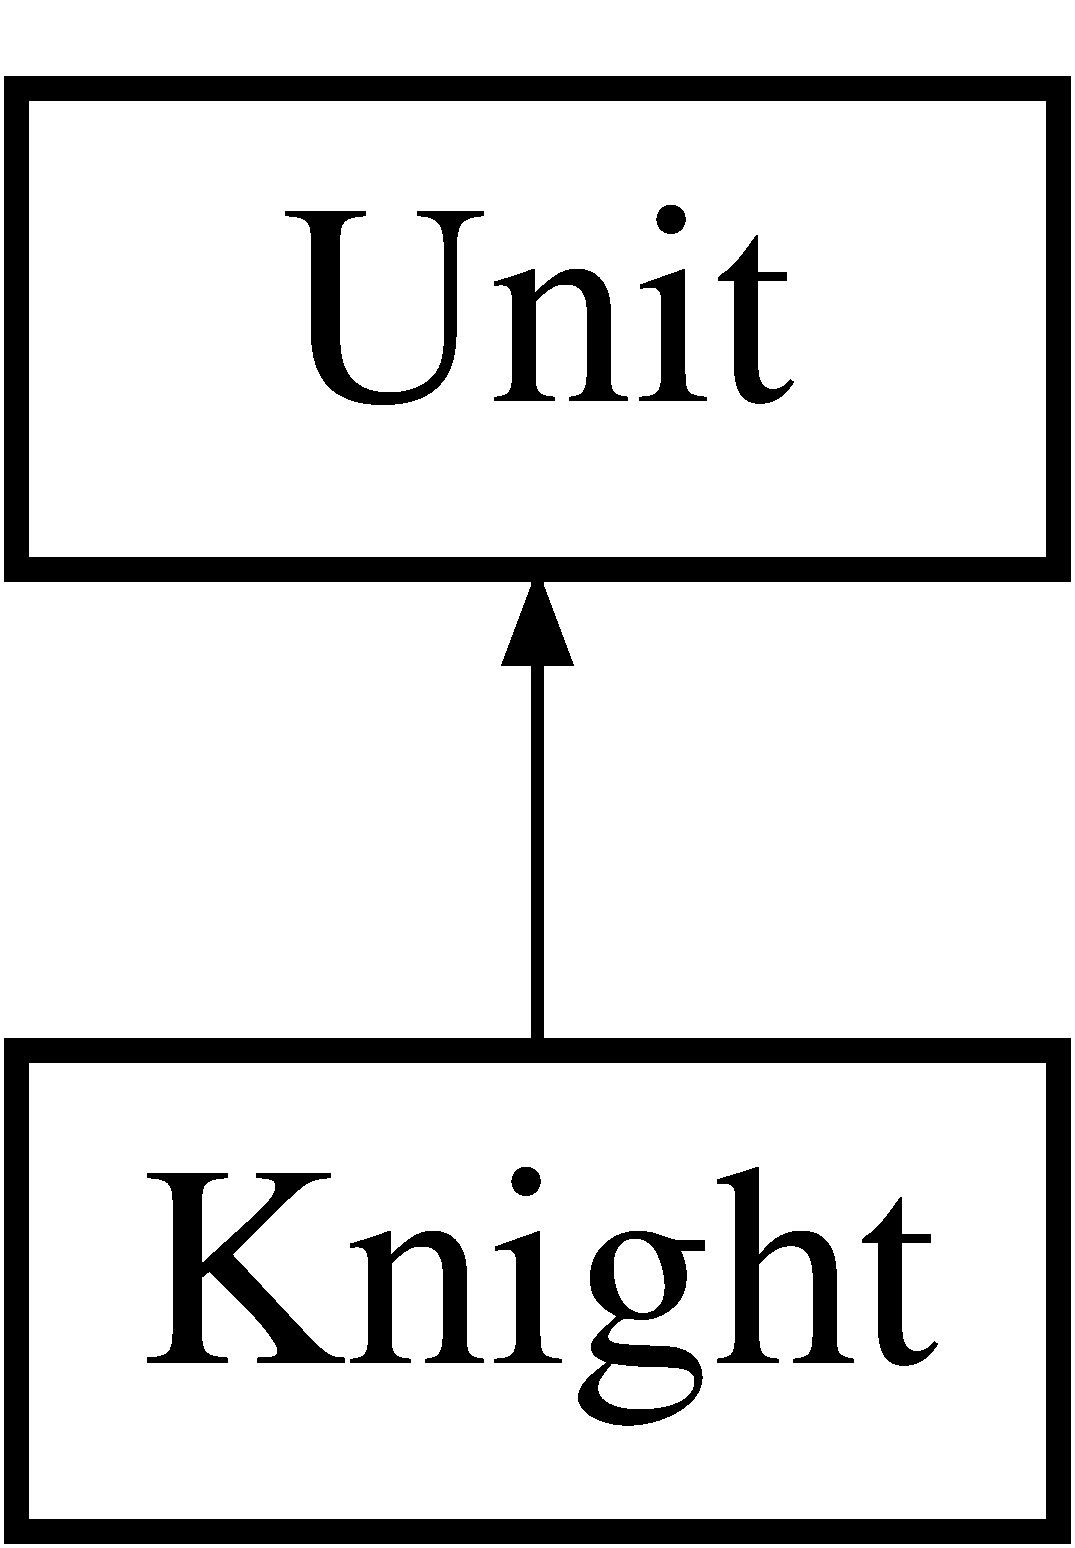
\includegraphics[height=2.000000cm]{classKnight}
\end{center}
\end{figure}
\subsection*{Fonctions membres publiques}
\begin{DoxyCompactItemize}
\item 
\hypertarget{classKnight_ae965f0055f4e556c17bdd1a48599c11c}{\hyperlink{classKnight_ae965f0055f4e556c17bdd1a48599c11c}{Knight} (unsigned int range, unsigned int ap, unsigned int mp, unsigned int hp, unsigned int dmgs, unsigned int cost, \hyperlink{classAttack}{Attack} $\ast$\hyperlink{classUnit_ac06b8f6e30f851f15a42d8a1d951034a}{attack}, \hyperlink{classHPLoss}{H\+P\+Loss} $\ast$\hyperlink{classUnit_a3090f43e2ee6a08587a160afaa26e7cd}{hp\+Loss}, \hyperlink{classMove}{Move} $\ast$\hyperlink{classUnit_a8c6bfbaf9bf204baec6ba3c11468ec2f}{move}, \hyperlink{classPosition}{Position} position, std\+::string image)}\label{classKnight_ae965f0055f4e556c17bdd1a48599c11c}

\begin{DoxyCompactList}\small\item\em Constructeur. \end{DoxyCompactList}\item 
std\+::string \hyperlink{classKnight_a62f9fd4f850fe38a491cbc31a9768e51}{classe} () const 
\begin{DoxyCompactList}\small\item\em Accesseur de la classe. \end{DoxyCompactList}\item 
\hyperlink{classUnit}{Unit} $\ast$ \hyperlink{classKnight_aff78fcbbd38c405b5c35f348160edce3}{clone} (\hyperlink{classPosition}{Position} position) const 
\begin{DoxyCompactList}\small\item\em construit un knight identique à la position donnée \end{DoxyCompactList}\item 
\hypertarget{classKnight_a3aa88288ca9bc2d319c5ee1b4569fdfc}{void \hyperlink{classKnight_a3aa88288ca9bc2d319c5ee1b4569fdfc}{afficher\+Infos} () const }\label{classKnight_a3aa88288ca9bc2d319c5ee1b4569fdfc}

\begin{DoxyCompactList}\small\item\em affiche les différentes informations sur l'archer \end{DoxyCompactList}\end{DoxyCompactItemize}
\subsection*{Membres hérités additionnels}


\subsection{Description détaillée}
Classe définissant un chevalier. 

Définition à la ligne 19 du fichier knight.\+hpp.



\subsection{Documentation des fonctions membres}
\hypertarget{classKnight_a62f9fd4f850fe38a491cbc31a9768e51}{\index{Knight@{Knight}!classe@{classe}}
\index{classe@{classe}!Knight@{Knight}}
\subsubsection[{classe}]{\setlength{\rightskip}{0pt plus 5cm}std\+::string Knight\+::classe (
\begin{DoxyParamCaption}
{}
\end{DoxyParamCaption}
) const\hspace{0.3cm}{\ttfamily [virtual]}}}\label{classKnight_a62f9fd4f850fe38a491cbc31a9768e51}


Accesseur de la classe. 

\begin{DoxyReturn}{Renvoie}
\char`\"{}knight\char`\"{} 
\end{DoxyReturn}


Implémente \hyperlink{classUnit_adac07557f9c0b9005709c62263625c2d}{Unit}.

\hypertarget{classKnight_aff78fcbbd38c405b5c35f348160edce3}{\index{Knight@{Knight}!clone@{clone}}
\index{clone@{clone}!Knight@{Knight}}
\subsubsection[{clone}]{\setlength{\rightskip}{0pt plus 5cm}{\bf Unit}$\ast$ Knight\+::clone (
\begin{DoxyParamCaption}
\item[{{\bf Position}}]{position}
\end{DoxyParamCaption}
) const\hspace{0.3cm}{\ttfamily [virtual]}}}\label{classKnight_aff78fcbbd38c405b5c35f348160edce3}


construit un knight identique à la position donnée 


\begin{DoxyParams}{Paramètres}
{\em position} & une position \\
\hline
\end{DoxyParams}
\begin{DoxyReturn}{Renvoie}
un knight 
\end{DoxyReturn}


Implémente \hyperlink{classUnit_a90304713be4b7cc73f59358190dd39d4}{Unit}.



La documentation de cette classe a été générée à partir du fichier suivant \+:\begin{DoxyCompactItemize}
\item 
src/\hyperlink{knight_8hpp}{knight.\+hpp}\end{DoxyCompactItemize}

\hypertarget{classMap}{\section{Référence de la classe Map}
\label{classMap}\index{Map@{Map}}
}


Classe permettant l'utilisation d'une map.  


\subsection*{Fonctions membres publiques}
\begin{DoxyCompactItemize}
\item 
\hypertarget{classMap_ae50ababdf30fcb0f5a10d38c1984eb75}{\hyperlink{classMap_ae50ababdf30fcb0f5a10d38c1984eb75}{Map} (std\+::vector$<$ std\+::vector$<$ unsigned int $>$$>$ tiles, std\+::vector$<$ \hyperlink{classPosition}{Position} $>$ starting\+Positions)}\label{classMap_ae50ababdf30fcb0f5a10d38c1984eb75}

\begin{DoxyCompactList}\small\item\em Constructeur. \end{DoxyCompactList}\item 
\hypertarget{classMap_aa403fbe09394ccf39747588f5168e3b2}{\hyperlink{classMap_aa403fbe09394ccf39747588f5168e3b2}{$\sim$\+Map} ()}\label{classMap_aa403fbe09394ccf39747588f5168e3b2}

\begin{DoxyCompactList}\small\item\em Destructeur. \end{DoxyCompactList}\item 
bool \hyperlink{classMap_a82b16c404e0e9a3f11619a4c040d6f74}{is\+Valid\+Path} (\hyperlink{classUnit}{Unit} $\ast$unit, \hyperlink{classPath}{Path} $\ast$path) const 
\begin{DoxyCompactList}\small\item\em Méthode qui teste si un chemin est valide pour une unité donnée. \end{DoxyCompactList}\item 
bool \hyperlink{classMap_a708c3a1b9b5e0771fedc078c8a22677a}{is\+Valid\+View\+Line} (\hyperlink{classUnit}{Unit} $\ast$unit, \hyperlink{classPosition}{Position} position) const 
\begin{DoxyCompactList}\small\item\em Méthode qui teste si une ligne de vue est valide pour une unité donnée. \end{DoxyCompactList}\item 
bool \hyperlink{classMap_a48877a918e3766b284120918b183b9d4}{is\+Valid\+Summon\+Position} (\hyperlink{classPosition}{Position} position, \hyperlink{classPlayer}{Player} $\ast$player) const 
\begin{DoxyCompactList}\small\item\em Méthode qui teste si une unité peut être invoquée à la position donnée. \end{DoxyCompactList}\item 
std\+::vector$<$ std\+::vector\\*
$<$ unsigned int $>$ $>$ \hyperlink{classMap_a902613cfaf7782f2212b088eccc2f0e7}{get\+Tiles} () const 
\begin{DoxyCompactList}\small\item\em Méthode qui retourne le tableau de tiles. \end{DoxyCompactList}\item 
\hyperlink{classUnit}{Unit} $\ast$ \hyperlink{classMap_a947916f15873cfad436bd8c156d8bcbf}{get\+Unit\+At} (\hyperlink{classPosition}{Position} position) const 
\begin{DoxyCompactList}\small\item\em Méthode qui retourne une unité présente à une position donnée. \end{DoxyCompactList}\item 
\hyperlink{classUnit}{Unit} $\ast$ \hyperlink{classMap_a5e9e5a63b3ffd5a7051d86cfb2ae2925}{get\+Unit} (unsigned int id) const 
\begin{DoxyCompactList}\small\item\em Accesseur de l'unité en fonction de son identifiant. \end{DoxyCompactList}\item 
bool \hyperlink{classMap_a150dfa9e7f3c31e8f7b8bdba6fe4a433}{is\+Unit} (unsigned int id) const 
\begin{DoxyCompactList}\small\item\em Permet de savoir si une unité existe. \end{DoxyCompactList}\item 
bool \hyperlink{classMap_ac1383a7aa9471f09d4a2f8708d872008}{is\+Unit\+At} (\hyperlink{classPosition}{Position} position) const 
\begin{DoxyCompactList}\small\item\em Méthode testant la présence d'une unité à une position donnée. \end{DoxyCompactList}\item 
\hyperlink{classBase}{Base} $\ast$ \hyperlink{classMap_a1943a0744e258950e341d368bdaec868}{get\+Base\+At} (\hyperlink{classPosition}{Position} position) const 
\begin{DoxyCompactList}\small\item\em Méthode qui retourne la base à la position donnée. \end{DoxyCompactList}\item 
bool \hyperlink{classMap_ad89412c547ebdcdd0831a8a7700c3f18}{is\+Base\+At} (\hyperlink{classPosition}{Position} position) const 
\begin{DoxyCompactList}\small\item\em Méthode qui teste si une base est présente à la position donnée. \end{DoxyCompactList}\item 
void \hyperlink{classMap_aee81c8e1fdb01828b733d392f5c1e068}{add\+Player} (\hyperlink{classPlayer}{Player} $\ast$player)
\begin{DoxyCompactList}\small\item\em Ajoute un joueur sur la map. \end{DoxyCompactList}\item 
std\+::map$<$ unsigned int, \hyperlink{classPlayer}{Player} $\ast$ $>$ $\ast$ \hyperlink{classMap_a8e1b744435056e5fff197956d1cfdfb7}{get\+Players} ()
\begin{DoxyCompactList}\small\item\em Accesseur de la map des joueurs. \end{DoxyCompactList}\item 
unsigned int \hyperlink{classMap_aaac0c6132fd80f0db5969833fed068c2}{get\+Size} () const 
\begin{DoxyCompactList}\small\item\em Accesseur de la taille de la map. \end{DoxyCompactList}\item 
bool \hyperlink{classMap_a1c5ffa96157a27bba9673135974b200c}{is\+Blocked} (\hyperlink{classPosition}{Position} position) const 
\begin{DoxyCompactList}\small\item\em Teste si la position donnée est bloquée. \end{DoxyCompactList}\item 
void \hyperlink{classMap_adeacfcfebbc96d2818acf8e10f56a36e}{die} (\hyperlink{classUnit}{Unit} $\ast$unit)
\begin{DoxyCompactList}\small\item\em Effectue les actions à la mort d'une unité \end{DoxyCompactList}\item 
\hypertarget{classMap_a8cf8d2999a559ac2d6d1e7bcc09ecafb}{void \hyperlink{classMap_a8cf8d2999a559ac2d6d1e7bcc09ecafb}{base\+Break} ()}\label{classMap_a8cf8d2999a559ac2d6d1e7bcc09ecafb}

\begin{DoxyCompactList}\small\item\em Effectue les actions à la mort d'une base. \end{DoxyCompactList}\item 
\hyperlink{classPlayer}{Player} $\ast$ \hyperlink{classMap_ab99bf425d6dd3c9de7db90d54308a9b7}{get\+Winner} ()
\begin{DoxyCompactList}\small\item\em Accesseur du gagnant de la partie. \end{DoxyCompactList}\end{DoxyCompactItemize}


\subsection{Description détaillée}
Classe permettant l'utilisation d'une map. 

Définition à la ligne 26 du fichier map.\+hpp.



\subsection{Documentation des fonctions membres}
\hypertarget{classMap_aee81c8e1fdb01828b733d392f5c1e068}{\index{Map@{Map}!add\+Player@{add\+Player}}
\index{add\+Player@{add\+Player}!Map@{Map}}
\subsubsection[{add\+Player}]{\setlength{\rightskip}{0pt plus 5cm}void Map\+::add\+Player (
\begin{DoxyParamCaption}
\item[{{\bf Player} $\ast$}]{player}
\end{DoxyParamCaption}
)}}\label{classMap_aee81c8e1fdb01828b733d392f5c1e068}


Ajoute un joueur sur la map. 


\begin{DoxyParams}{Paramètres}
{\em player} & le joueur à ajouté \\
\hline
\end{DoxyParams}
\hypertarget{classMap_adeacfcfebbc96d2818acf8e10f56a36e}{\index{Map@{Map}!die@{die}}
\index{die@{die}!Map@{Map}}
\subsubsection[{die}]{\setlength{\rightskip}{0pt plus 5cm}void Map\+::die (
\begin{DoxyParamCaption}
\item[{{\bf Unit} $\ast$}]{unit}
\end{DoxyParamCaption}
)}}\label{classMap_adeacfcfebbc96d2818acf8e10f56a36e}


Effectue les actions à la mort d'une unité 


\begin{DoxyParams}{Paramètres}
{\em unit} & une unité \\
\hline
\end{DoxyParams}
\hypertarget{classMap_a1943a0744e258950e341d368bdaec868}{\index{Map@{Map}!get\+Base\+At@{get\+Base\+At}}
\index{get\+Base\+At@{get\+Base\+At}!Map@{Map}}
\subsubsection[{get\+Base\+At}]{\setlength{\rightskip}{0pt plus 5cm}{\bf Base}$\ast$ Map\+::get\+Base\+At (
\begin{DoxyParamCaption}
\item[{{\bf Position}}]{position}
\end{DoxyParamCaption}
) const}}\label{classMap_a1943a0744e258950e341d368bdaec868}


Méthode qui retourne la base à la position donnée. 


\begin{DoxyParams}{Paramètres}
{\em position} & la position \\
\hline
\end{DoxyParams}
\begin{DoxyReturn}{Renvoie}
la base 
\end{DoxyReturn}
\hypertarget{classMap_a8e1b744435056e5fff197956d1cfdfb7}{\index{Map@{Map}!get\+Players@{get\+Players}}
\index{get\+Players@{get\+Players}!Map@{Map}}
\subsubsection[{get\+Players}]{\setlength{\rightskip}{0pt plus 5cm}std\+::map$<$unsigned int, {\bf Player}$\ast$$>$$\ast$ Map\+::get\+Players (
\begin{DoxyParamCaption}
{}
\end{DoxyParamCaption}
)}}\label{classMap_a8e1b744435056e5fff197956d1cfdfb7}


Accesseur de la map des joueurs. 

\begin{DoxyReturn}{Renvoie}
une map id -\/$>$ joueur contenant tous les joueurs 
\end{DoxyReturn}
\hypertarget{classMap_aaac0c6132fd80f0db5969833fed068c2}{\index{Map@{Map}!get\+Size@{get\+Size}}
\index{get\+Size@{get\+Size}!Map@{Map}}
\subsubsection[{get\+Size}]{\setlength{\rightskip}{0pt plus 5cm}unsigned int Map\+::get\+Size (
\begin{DoxyParamCaption}
{}
\end{DoxyParamCaption}
) const}}\label{classMap_aaac0c6132fd80f0db5969833fed068c2}


Accesseur de la taille de la map. 

\begin{DoxyReturn}{Renvoie}
un unsigned int 
\end{DoxyReturn}
\hypertarget{classMap_a902613cfaf7782f2212b088eccc2f0e7}{\index{Map@{Map}!get\+Tiles@{get\+Tiles}}
\index{get\+Tiles@{get\+Tiles}!Map@{Map}}
\subsubsection[{get\+Tiles}]{\setlength{\rightskip}{0pt plus 5cm}std\+::vector$<$std\+::vector$<$unsigned int$>$ $>$ Map\+::get\+Tiles (
\begin{DoxyParamCaption}
{}
\end{DoxyParamCaption}
) const}}\label{classMap_a902613cfaf7782f2212b088eccc2f0e7}


Méthode qui retourne le tableau de tiles. 

\begin{DoxyReturn}{Renvoie}
le tableau des tiles 
\end{DoxyReturn}
\hypertarget{classMap_a5e9e5a63b3ffd5a7051d86cfb2ae2925}{\index{Map@{Map}!get\+Unit@{get\+Unit}}
\index{get\+Unit@{get\+Unit}!Map@{Map}}
\subsubsection[{get\+Unit}]{\setlength{\rightskip}{0pt plus 5cm}{\bf Unit}$\ast$ Map\+::get\+Unit (
\begin{DoxyParamCaption}
\item[{unsigned int}]{id}
\end{DoxyParamCaption}
) const}}\label{classMap_a5e9e5a63b3ffd5a7051d86cfb2ae2925}


Accesseur de l'unité en fonction de son identifiant. 


\begin{DoxyParams}{Paramètres}
{\em id} & l'identifiant de l'unité \\
\hline
\end{DoxyParams}
\begin{DoxyReturn}{Renvoie}
l'unité qui possède id comme identifiant 
\end{DoxyReturn}
\hypertarget{classMap_a947916f15873cfad436bd8c156d8bcbf}{\index{Map@{Map}!get\+Unit\+At@{get\+Unit\+At}}
\index{get\+Unit\+At@{get\+Unit\+At}!Map@{Map}}
\subsubsection[{get\+Unit\+At}]{\setlength{\rightskip}{0pt plus 5cm}{\bf Unit}$\ast$ Map\+::get\+Unit\+At (
\begin{DoxyParamCaption}
\item[{{\bf Position}}]{position}
\end{DoxyParamCaption}
) const}}\label{classMap_a947916f15873cfad436bd8c156d8bcbf}


Méthode qui retourne une unité présente à une position donnée. 


\begin{DoxyParams}{Paramètres}
{\em position} & la position à laquelle on va récupèrer l'unité \\
\hline
\end{DoxyParams}
\begin{DoxyReturn}{Renvoie}
l'unité présente à la position donnée 
\end{DoxyReturn}
\hypertarget{classMap_ab99bf425d6dd3c9de7db90d54308a9b7}{\index{Map@{Map}!get\+Winner@{get\+Winner}}
\index{get\+Winner@{get\+Winner}!Map@{Map}}
\subsubsection[{get\+Winner}]{\setlength{\rightskip}{0pt plus 5cm}{\bf Player}$\ast$ Map\+::get\+Winner (
\begin{DoxyParamCaption}
{}
\end{DoxyParamCaption}
)}}\label{classMap_ab99bf425d6dd3c9de7db90d54308a9b7}


Accesseur du gagnant de la partie. 

\begin{DoxyReturn}{Renvoie}
une joueur 
\end{DoxyReturn}
\hypertarget{classMap_ad89412c547ebdcdd0831a8a7700c3f18}{\index{Map@{Map}!is\+Base\+At@{is\+Base\+At}}
\index{is\+Base\+At@{is\+Base\+At}!Map@{Map}}
\subsubsection[{is\+Base\+At}]{\setlength{\rightskip}{0pt plus 5cm}bool Map\+::is\+Base\+At (
\begin{DoxyParamCaption}
\item[{{\bf Position}}]{position}
\end{DoxyParamCaption}
) const}}\label{classMap_ad89412c547ebdcdd0831a8a7700c3f18}


Méthode qui teste si une base est présente à la position donnée. 


\begin{DoxyParams}{Paramètres}
{\em position} & la position \\
\hline
\end{DoxyParams}
\begin{DoxyReturn}{Renvoie}
vrai si il y a une base 
\end{DoxyReturn}
\hypertarget{classMap_a1c5ffa96157a27bba9673135974b200c}{\index{Map@{Map}!is\+Blocked@{is\+Blocked}}
\index{is\+Blocked@{is\+Blocked}!Map@{Map}}
\subsubsection[{is\+Blocked}]{\setlength{\rightskip}{0pt plus 5cm}bool Map\+::is\+Blocked (
\begin{DoxyParamCaption}
\item[{{\bf Position}}]{position}
\end{DoxyParamCaption}
) const}}\label{classMap_a1c5ffa96157a27bba9673135974b200c}


Teste si la position donnée est bloquée. 


\begin{DoxyParams}{Paramètres}
{\em position} & une position \\
\hline
\end{DoxyParams}
\begin{DoxyReturn}{Renvoie}
vrai si la position est bloquée, faux sinon 
\end{DoxyReturn}
\hypertarget{classMap_a150dfa9e7f3c31e8f7b8bdba6fe4a433}{\index{Map@{Map}!is\+Unit@{is\+Unit}}
\index{is\+Unit@{is\+Unit}!Map@{Map}}
\subsubsection[{is\+Unit}]{\setlength{\rightskip}{0pt plus 5cm}bool Map\+::is\+Unit (
\begin{DoxyParamCaption}
\item[{unsigned int}]{id}
\end{DoxyParamCaption}
) const}}\label{classMap_a150dfa9e7f3c31e8f7b8bdba6fe4a433}


Permet de savoir si une unité existe. 


\begin{DoxyParams}{Paramètres}
{\em id} & l'identifiant de l'unité \\
\hline
\end{DoxyParams}
\begin{DoxyReturn}{Renvoie}
vrai si l'unité existe 
\end{DoxyReturn}
\hypertarget{classMap_ac1383a7aa9471f09d4a2f8708d872008}{\index{Map@{Map}!is\+Unit\+At@{is\+Unit\+At}}
\index{is\+Unit\+At@{is\+Unit\+At}!Map@{Map}}
\subsubsection[{is\+Unit\+At}]{\setlength{\rightskip}{0pt plus 5cm}bool Map\+::is\+Unit\+At (
\begin{DoxyParamCaption}
\item[{{\bf Position}}]{position}
\end{DoxyParamCaption}
) const}}\label{classMap_ac1383a7aa9471f09d4a2f8708d872008}


Méthode testant la présence d'une unité à une position donnée. 


\begin{DoxyParams}{Paramètres}
{\em position} & la position a laquelle on veut savoir si une unité est présente \\
\hline
\end{DoxyParams}
\begin{DoxyReturn}{Renvoie}
vrai s'il y a une unité à la position donnée 
\end{DoxyReturn}
\hypertarget{classMap_a82b16c404e0e9a3f11619a4c040d6f74}{\index{Map@{Map}!is\+Valid\+Path@{is\+Valid\+Path}}
\index{is\+Valid\+Path@{is\+Valid\+Path}!Map@{Map}}
\subsubsection[{is\+Valid\+Path}]{\setlength{\rightskip}{0pt plus 5cm}bool Map\+::is\+Valid\+Path (
\begin{DoxyParamCaption}
\item[{{\bf Unit} $\ast$}]{unit, }
\item[{{\bf Path} $\ast$}]{path}
\end{DoxyParamCaption}
) const}}\label{classMap_a82b16c404e0e9a3f11619a4c040d6f74}


Méthode qui teste si un chemin est valide pour une unité donnée. 


\begin{DoxyParams}{Paramètres}
{\em unit} & l'unité permetant de savoir l'emplacement de départ du chemin \\
\hline
{\em path} & le chemin à tester \\
\hline
\end{DoxyParams}
\begin{DoxyReturn}{Renvoie}
vrai si le chemin est valide 
\end{DoxyReturn}
\hypertarget{classMap_a48877a918e3766b284120918b183b9d4}{\index{Map@{Map}!is\+Valid\+Summon\+Position@{is\+Valid\+Summon\+Position}}
\index{is\+Valid\+Summon\+Position@{is\+Valid\+Summon\+Position}!Map@{Map}}
\subsubsection[{is\+Valid\+Summon\+Position}]{\setlength{\rightskip}{0pt plus 5cm}bool Map\+::is\+Valid\+Summon\+Position (
\begin{DoxyParamCaption}
\item[{{\bf Position}}]{position, }
\item[{{\bf Player} $\ast$}]{player}
\end{DoxyParamCaption}
) const}}\label{classMap_a48877a918e3766b284120918b183b9d4}


Méthode qui teste si une unité peut être invoquée à la position donnée. 


\begin{DoxyParams}{Paramètres}
{\em position} & la position d'invocation \\
\hline
{\em player} & le joueur qui invoque \\
\hline
\end{DoxyParams}
\begin{DoxyReturn}{Renvoie}
vrai si l'unité peut être invoquée à la position p 
\end{DoxyReturn}
\hypertarget{classMap_a708c3a1b9b5e0771fedc078c8a22677a}{\index{Map@{Map}!is\+Valid\+View\+Line@{is\+Valid\+View\+Line}}
\index{is\+Valid\+View\+Line@{is\+Valid\+View\+Line}!Map@{Map}}
\subsubsection[{is\+Valid\+View\+Line}]{\setlength{\rightskip}{0pt plus 5cm}bool Map\+::is\+Valid\+View\+Line (
\begin{DoxyParamCaption}
\item[{{\bf Unit} $\ast$}]{unit, }
\item[{{\bf Position}}]{position}
\end{DoxyParamCaption}
) const}}\label{classMap_a708c3a1b9b5e0771fedc078c8a22677a}


Méthode qui teste si une ligne de vue est valide pour une unité donnée. 


\begin{DoxyParams}{Paramètres}
{\em unit} & l'unité permetant de savoir l'emplacement de départ de l'action \\
\hline
{\em position} & la position ou l'action doit être effectuée \\
\hline
\end{DoxyParams}
\begin{DoxyReturn}{Renvoie}
vrai si la ligne de vue est valide 
\end{DoxyReturn}


La documentation de cette classe a été générée à partir du fichier suivant \+:\begin{DoxyCompactItemize}
\item 
src/\hyperlink{map_8hpp}{map.\+hpp}\end{DoxyCompactItemize}

\hypertarget{classMove}{\section{Référence de la classe Move}
\label{classMove}\index{Move@{Move}}
}


Classe virtuelle pure permettant l'utilisation de différents comportement de déplacements selon l'unité. Elle est utilisée dans le cadre du pattern Strategy.  




{\ttfamily \#include $<$move.\+hpp$>$}

Graphe d'héritage de Move\+:\begin{figure}[H]
\begin{center}
\leavevmode
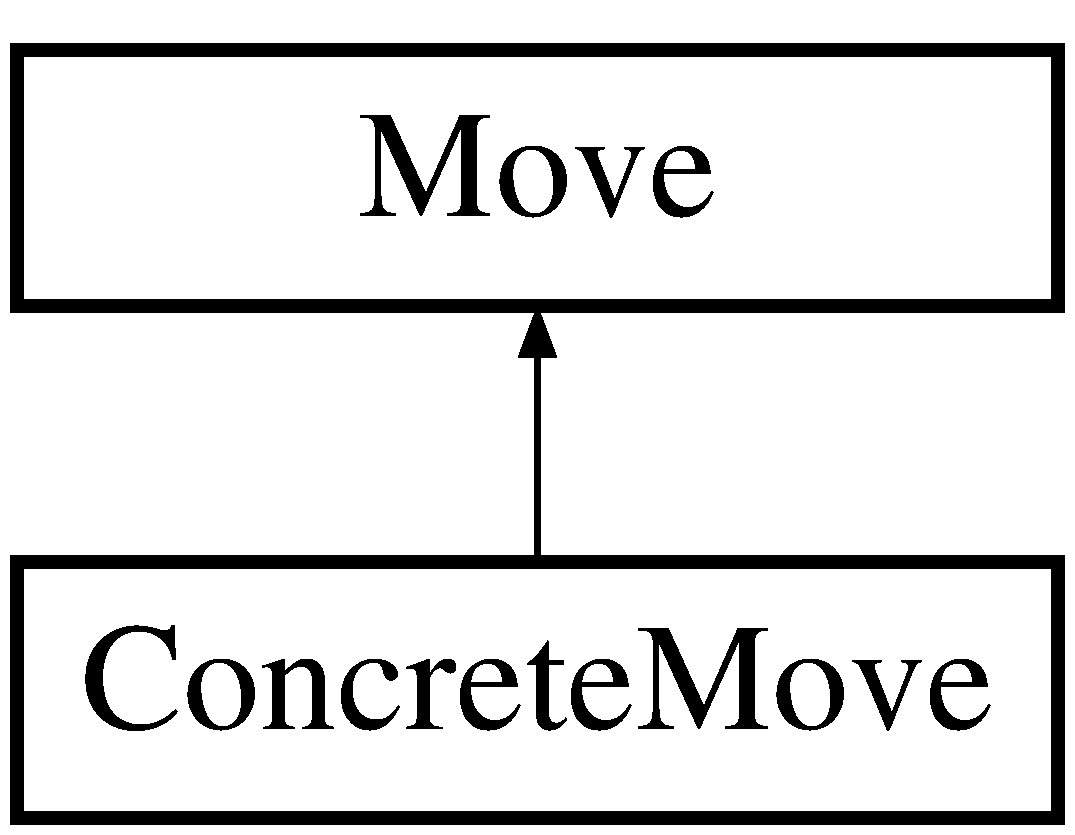
\includegraphics[height=2.000000cm]{classMove}
\end{center}
\end{figure}
\subsection*{Fonctions membres publiques}
\begin{DoxyCompactItemize}
\item 
virtual void \hyperlink{classMove_ace4540308f0bbd21d71a18b2ff7c972d}{move} (\hyperlink{classPath}{Path} $\ast$path, \hyperlink{classMap}{Map} $\ast$map, \hyperlink{classUnit}{Unit} $\ast$u)=0
\begin{DoxyCompactList}\small\item\em Destructeur (évite les warnings) \end{DoxyCompactList}\end{DoxyCompactItemize}


\subsection{Description détaillée}
Classe virtuelle pure permettant l'utilisation de différents comportement de déplacements selon l'unité. Elle est utilisée dans le cadre du pattern Strategy. 

Définition à la ligne 21 du fichier move.\+hpp.



\subsection{Documentation des fonctions membres}
\hypertarget{classMove_ace4540308f0bbd21d71a18b2ff7c972d}{\index{Move@{Move}!move@{move}}
\index{move@{move}!Move@{Move}}
\subsubsection[{move}]{\setlength{\rightskip}{0pt plus 5cm}virtual void Move\+::move (
\begin{DoxyParamCaption}
\item[{{\bf Path} $\ast$}]{path, }
\item[{{\bf Map} $\ast$}]{map, }
\item[{{\bf Unit} $\ast$}]{u}
\end{DoxyParamCaption}
)\hspace{0.3cm}{\ttfamily [pure virtual]}}}\label{classMove_ace4540308f0bbd21d71a18b2ff7c972d}


Destructeur (évite les warnings) 

méthode virtuelle pure de déplacement d'une unité 
\begin{DoxyParams}{Paramètres}
{\em path} & un chemin \\
\hline
{\em map} & une map \\
\hline
{\em u} & une unité \\
\hline
\end{DoxyParams}


Implémenté dans \hyperlink{classConcreteMove_adbbcf93faa6dad1660a922618b905ff1}{Concrete\+Move}.



La documentation de cette classe a été générée à partir du fichier suivant \+:\begin{DoxyCompactItemize}
\item 
src/\hyperlink{move_8hpp}{move.\+hpp}\end{DoxyCompactItemize}

\hypertarget{classObserver}{\section{Référence de la classe Observer}
\label{classObserver}\index{Observer@{Observer}}
}
Graphe d'héritage de Observer\+:\begin{figure}[H]
\begin{center}
\leavevmode
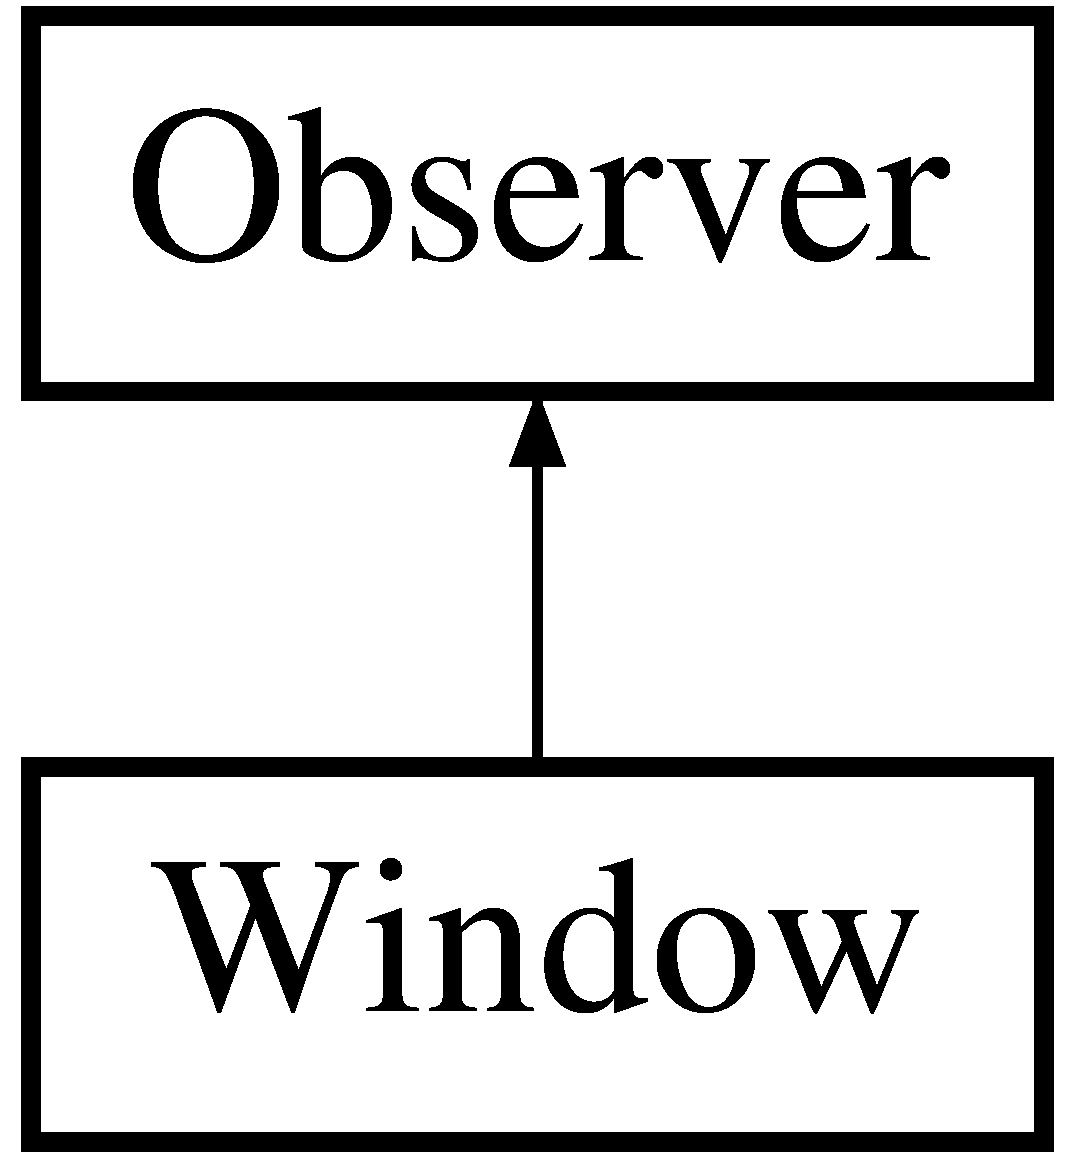
\includegraphics[height=2.000000cm]{classObserver}
\end{center}
\end{figure}
\subsection*{Fonctions membres publiques}
\begin{DoxyCompactItemize}
\item 
virtual void \hyperlink{classObserver_a27884af3c43e814cc1e613cd593efb55}{update} (\hyperlink{classSubject}{Subject} $\ast$s)=0
\begin{DoxyCompactList}\small\item\em méthode appelée lors de la mise a jour du sujet \end{DoxyCompactList}\end{DoxyCompactItemize}


\subsection{Description détaillée}


Définition à la ligne 18 du fichier observer.\+hpp.



\subsection{Documentation des fonctions membres}
\hypertarget{classObserver_a27884af3c43e814cc1e613cd593efb55}{\index{Observer@{Observer}!update@{update}}
\index{update@{update}!Observer@{Observer}}
\subsubsection[{update}]{\setlength{\rightskip}{0pt plus 5cm}virtual void Observer\+::update (
\begin{DoxyParamCaption}
\item[{{\bf Subject} $\ast$}]{s}
\end{DoxyParamCaption}
)\hspace{0.3cm}{\ttfamily [pure virtual]}}}\label{classObserver_a27884af3c43e814cc1e613cd593efb55}


méthode appelée lors de la mise a jour du sujet 


\begin{DoxyParams}{Paramètres}
{\em s} & un sujet \\
\hline
\end{DoxyParams}


Implémenté dans \hyperlink{classWindow_a23acb0c66756df8121ce5d54a8c28d72}{Window}.



La documentation de cette classe a été générée à partir du fichier suivant \+:\begin{DoxyCompactItemize}
\item 
src/\hyperlink{observer_8hpp}{observer.\+hpp}\end{DoxyCompactItemize}

\hypertarget{classObserveur}{\section{Référence de la classe Observeur}
\label{classObserveur}\index{Observeur@{Observeur}}
}


Classe abstraite définissant le comportement des toutes les classes observatrices.  




\subsection{Description détaillée}
Classe abstraite définissant le comportement des toutes les classes observatrices. 

Définition à la ligne 11 du fichier observer.\+hpp.



La documentation de cette classe a été générée à partir du fichier suivant \+:\begin{DoxyCompactItemize}
\item 
src/\hyperlink{observer_8hpp}{observer.\+hpp}\end{DoxyCompactItemize}

\hypertarget{classPath}{\section{Référence de la classe Path}
\label{classPath}\index{Path@{Path}}
}


Classe implémentant un chemin (path) sur la map.  




{\ttfamily \#include $<$path.\+hpp$>$}

\subsection*{Fonctions membres publiques}
\begin{DoxyCompactItemize}
\item 
\hypertarget{classPath_af2fb51479b719021bbdb3a1d540d1c78}{void \hyperlink{classPath_af2fb51479b719021bbdb3a1d540d1c78}{push\+Pos} (\hyperlink{classPosition}{Position} pos)}\label{classPath_af2fb51479b719021bbdb3a1d540d1c78}

\begin{DoxyCompactList}\small\item\em ajoute une position au vector \end{DoxyCompactList}\item 
\hyperlink{classPosition}{Position} \hyperlink{classPath_a3ba977222e0dbfbf731bdf1d4856f5de}{pop\+Pos} ()
\begin{DoxyCompactList}\small\item\em retire une position au vector \end{DoxyCompactList}\item 
\hyperlink{classPosition}{Position} \hyperlink{classPath_a1d790239748af16e157aaa04ce262a36}{get\+Position} (unsigned int i) const 
\begin{DoxyCompactList}\small\item\em accesseur des éléments du vector \end{DoxyCompactList}\item 
unsigned int \hyperlink{classPath_a5a0eb3303c0e3fed707c9e0cf6f31257}{size} () const 
\begin{DoxyCompactList}\small\item\em calcule la taille du vector \end{DoxyCompactList}\item 
\hypertarget{classPath_a3b2b7259396354a7a79245065a363373}{\hyperlink{classPosition}{Position} \hyperlink{classPath_a3b2b7259396354a7a79245065a363373}{operator\mbox{[}$\,$\mbox{]}} (unsigned int const \&i)}\label{classPath_a3b2b7259396354a7a79245065a363373}

\begin{DoxyCompactList}\small\item\em redéfinition de l'accesseur aux case du tableau \end{DoxyCompactList}\end{DoxyCompactItemize}


\subsection{Description détaillée}
Classe implémentant un chemin (path) sur la map. 

Définition à la ligne 21 du fichier path.\+hpp.



\subsection{Documentation des fonctions membres}
\hypertarget{classPath_a1d790239748af16e157aaa04ce262a36}{\index{Path@{Path}!get\+Position@{get\+Position}}
\index{get\+Position@{get\+Position}!Path@{Path}}
\subsubsection[{get\+Position}]{\setlength{\rightskip}{0pt plus 5cm}{\bf Position} Path\+::get\+Position (
\begin{DoxyParamCaption}
\item[{unsigned int}]{i}
\end{DoxyParamCaption}
) const}}\label{classPath_a1d790239748af16e157aaa04ce262a36}


accesseur des éléments du vector 

\begin{DoxyReturn}{Renvoie}
la position à l'indice i 
\end{DoxyReturn}
\hypertarget{classPath_a3ba977222e0dbfbf731bdf1d4856f5de}{\index{Path@{Path}!pop\+Pos@{pop\+Pos}}
\index{pop\+Pos@{pop\+Pos}!Path@{Path}}
\subsubsection[{pop\+Pos}]{\setlength{\rightskip}{0pt plus 5cm}{\bf Position} Path\+::pop\+Pos (
\begin{DoxyParamCaption}
{}
\end{DoxyParamCaption}
)}}\label{classPath_a3ba977222e0dbfbf731bdf1d4856f5de}


retire une position au vector 

\begin{DoxyReturn}{Renvoie}
la position retirée 
\end{DoxyReturn}
\hypertarget{classPath_a5a0eb3303c0e3fed707c9e0cf6f31257}{\index{Path@{Path}!size@{size}}
\index{size@{size}!Path@{Path}}
\subsubsection[{size}]{\setlength{\rightskip}{0pt plus 5cm}unsigned int Path\+::size (
\begin{DoxyParamCaption}
{}
\end{DoxyParamCaption}
) const}}\label{classPath_a5a0eb3303c0e3fed707c9e0cf6f31257}


calcule la taille du vector 

\begin{DoxyReturn}{Renvoie}
la taille de \+\_\+path 
\end{DoxyReturn}


La documentation de cette classe a été générée à partir du fichier suivant \+:\begin{DoxyCompactItemize}
\item 
src/\hyperlink{path_8hpp}{path.\+hpp}\end{DoxyCompactItemize}

\hypertarget{classPlayer}{\section{Référence de la classe Player}
\label{classPlayer}\index{Player@{Player}}
}


Classe définissant un joueur.  




{\ttfamily \#include $<$player.\+hpp$>$}

\subsection*{Fonctions membres publiques}
\begin{DoxyCompactItemize}
\item 
\hypertarget{classPlayer_a64124cbd4f373c5b7ebec1aaee471e06}{\hyperlink{classPlayer_a64124cbd4f373c5b7ebec1aaee471e06}{Player} (std\+::string name, unsigned int golds, \hyperlink{classBase}{Base} $\ast$base)}\label{classPlayer_a64124cbd4f373c5b7ebec1aaee471e06}

\begin{DoxyCompactList}\small\item\em Constructeur. \end{DoxyCompactList}\item 
\hypertarget{classPlayer_a749d2c00e1fe0f5c2746f7505a58c062}{\hyperlink{classPlayer_a749d2c00e1fe0f5c2746f7505a58c062}{$\sim$\+Player} ()}\label{classPlayer_a749d2c00e1fe0f5c2746f7505a58c062}

\begin{DoxyCompactList}\small\item\em Destructeur. \end{DoxyCompactList}\item 
unsigned int \hyperlink{classPlayer_a6e7e67674bf8f2896cff3ef7f4fa7e0d}{get\+Id} () const 
\begin{DoxyCompactList}\small\item\em Accesseur de l'identifiant. \end{DoxyCompactList}\item 
std\+::string \hyperlink{classPlayer_ad4c6a95f1cf69c44d0c585465b101c70}{get\+Name} () const 
\begin{DoxyCompactList}\small\item\em Accesseur du nom. \end{DoxyCompactList}\item 
unsigned int \hyperlink{classPlayer_a5a300fd8e477c6d9f19266763970daaf}{get\+Golds} () const 
\begin{DoxyCompactList}\small\item\em Accesseur du nombre de golds. \end{DoxyCompactList}\item 
std\+::map$<$ unsigned int, \hyperlink{classUnit}{Unit} $\ast$ $>$ $\ast$ \hyperlink{classPlayer_a1184d2d25acc16958d0e7710fe0f00ec}{get\+Units} ()
\begin{DoxyCompactList}\small\item\em Accesseur du tableau des unités. \end{DoxyCompactList}\item 
\hyperlink{classBase}{Base} $\ast$ \hyperlink{classPlayer_a1a3f0608b817489ecce50a53da619270}{get\+Base} () const 
\begin{DoxyCompactList}\small\item\em Accesseur de la base. \end{DoxyCompactList}\item 
void \hyperlink{classPlayer_a8963d12d2c4e47cd073ed9829dd86c79}{summon} (\hyperlink{classUnit}{Unit} $\ast$unit)
\begin{DoxyCompactList}\small\item\em Méthode qui permet à un joueur d'invoquer une unité donnée à une position donnée. \end{DoxyCompactList}\item 
void \hyperlink{classPlayer_a96a07d17d57a83a43c7f639803e02f49}{kill} (\hyperlink{classUnit}{Unit} $\ast$unit)
\begin{DoxyCompactList}\small\item\em Retire l'unité de la liste des unité \end{DoxyCompactList}\item 
void \hyperlink{classPlayer_a3b8380f4cd58fe75a985c0c2e3f32c8a}{add\+Golds} (unsigned int golds)
\begin{DoxyCompactList}\small\item\em Méthode qui crédite l'argent d'un joueur de la somme donnée. \end{DoxyCompactList}\item 
void \hyperlink{classPlayer_a375e40b8080b58b5fe5296d44ab74f8e}{rm\+Golds} (unsigned int golds)
\begin{DoxyCompactList}\small\item\em Méthode qui débite l'argent d'un joueur de la somme donnée. \end{DoxyCompactList}\item 
\hypertarget{classPlayer_a93eb96604ac6b679bda65a8bb18083ee}{void \hyperlink{classPlayer_a93eb96604ac6b679bda65a8bb18083ee}{affiche\+Golds} ()}\label{classPlayer_a93eb96604ac6b679bda65a8bb18083ee}

\begin{DoxyCompactList}\small\item\em Méthode qui affiche la quantité d'argent du joueur. \end{DoxyCompactList}\item 
void \hyperlink{classPlayer_aa25996d64c6b562ac737c548bdc687a6}{set\+Next} (\hyperlink{classPlayer}{Player} $\ast$next)
\begin{DoxyCompactList}\small\item\em Modifie le joueur suivant dans l'ordre du jeu. \end{DoxyCompactList}\item 
\hyperlink{classPlayer}{Player} $\ast$ \hyperlink{classPlayer_a6f9f2357bacaeb64a926b98da355afd7}{get\+Next} () const 
\begin{DoxyCompactList}\small\item\em Retourne le joueur suivant dans l'ordre du jeu. \end{DoxyCompactList}\item 
\hyperlink{classUnit}{Unit} $\ast$ \hyperlink{classPlayer_af8d6f506784f7dc1c1dd49db84f31831}{get\+Unit} (unsigned int id) const 
\begin{DoxyCompactList}\small\item\em Retourne l'unité du joueur en fonction du paramètre. \end{DoxyCompactList}\item 
\hypertarget{classPlayer_a2e72d8952b9fa896bd750e24ec5c6497}{void \hyperlink{classPlayer_a2e72d8952b9fa896bd750e24ec5c6497}{affiche\+Units} ()}\label{classPlayer_a2e72d8952b9fa896bd750e24ec5c6497}

\begin{DoxyCompactList}\small\item\em Affiche toutes les unité du joueur. \end{DoxyCompactList}\item 
\hypertarget{classPlayer_a8a6677e3a5b23a764ee224336fc61dba}{void \hyperlink{classPlayer_a8a6677e3a5b23a764ee224336fc61dba}{end\+Turn} ()}\label{classPlayer_a8a6677e3a5b23a764ee224336fc61dba}

\begin{DoxyCompactList}\small\item\em Méthode qui appelle \hyperlink{classPlayer_a8a6677e3a5b23a764ee224336fc61dba}{end\+Turn()} de chaque unité \end{DoxyCompactList}\end{DoxyCompactItemize}


\subsection{Description détaillée}
Classe définissant un joueur. 

Définition à la ligne 22 du fichier player.\+hpp.



\subsection{Documentation des fonctions membres}
\hypertarget{classPlayer_a3b8380f4cd58fe75a985c0c2e3f32c8a}{\index{Player@{Player}!add\+Golds@{add\+Golds}}
\index{add\+Golds@{add\+Golds}!Player@{Player}}
\subsubsection[{add\+Golds}]{\setlength{\rightskip}{0pt plus 5cm}void Player\+::add\+Golds (
\begin{DoxyParamCaption}
\item[{unsigned int}]{golds}
\end{DoxyParamCaption}
)}}\label{classPlayer_a3b8380f4cd58fe75a985c0c2e3f32c8a}


Méthode qui crédite l'argent d'un joueur de la somme donnée. 


\begin{DoxyParams}{Paramètres}
{\em golds} & la somme à créditer \\
\hline
\end{DoxyParams}
\hypertarget{classPlayer_a1a3f0608b817489ecce50a53da619270}{\index{Player@{Player}!get\+Base@{get\+Base}}
\index{get\+Base@{get\+Base}!Player@{Player}}
\subsubsection[{get\+Base}]{\setlength{\rightskip}{0pt plus 5cm}{\bf Base}$\ast$ Player\+::get\+Base (
\begin{DoxyParamCaption}
{}
\end{DoxyParamCaption}
) const}}\label{classPlayer_a1a3f0608b817489ecce50a53da619270}


Accesseur de la base. 

\begin{DoxyReturn}{Renvoie}
la base du joueur 
\end{DoxyReturn}
\hypertarget{classPlayer_a5a300fd8e477c6d9f19266763970daaf}{\index{Player@{Player}!get\+Golds@{get\+Golds}}
\index{get\+Golds@{get\+Golds}!Player@{Player}}
\subsubsection[{get\+Golds}]{\setlength{\rightskip}{0pt plus 5cm}unsigned int Player\+::get\+Golds (
\begin{DoxyParamCaption}
{}
\end{DoxyParamCaption}
) const}}\label{classPlayer_a5a300fd8e477c6d9f19266763970daaf}


Accesseur du nombre de golds. 

\begin{DoxyReturn}{Renvoie}
le nombre de golds du joueur 
\end{DoxyReturn}
\hypertarget{classPlayer_a6e7e67674bf8f2896cff3ef7f4fa7e0d}{\index{Player@{Player}!get\+Id@{get\+Id}}
\index{get\+Id@{get\+Id}!Player@{Player}}
\subsubsection[{get\+Id}]{\setlength{\rightskip}{0pt plus 5cm}unsigned int Player\+::get\+Id (
\begin{DoxyParamCaption}
{}
\end{DoxyParamCaption}
) const}}\label{classPlayer_a6e7e67674bf8f2896cff3ef7f4fa7e0d}


Accesseur de l'identifiant. 

\begin{DoxyReturn}{Renvoie}
l'identifiant du joueur 
\end{DoxyReturn}
\hypertarget{classPlayer_ad4c6a95f1cf69c44d0c585465b101c70}{\index{Player@{Player}!get\+Name@{get\+Name}}
\index{get\+Name@{get\+Name}!Player@{Player}}
\subsubsection[{get\+Name}]{\setlength{\rightskip}{0pt plus 5cm}std\+::string Player\+::get\+Name (
\begin{DoxyParamCaption}
{}
\end{DoxyParamCaption}
) const}}\label{classPlayer_ad4c6a95f1cf69c44d0c585465b101c70}


Accesseur du nom. 

\begin{DoxyReturn}{Renvoie}
le nom du joueur 
\end{DoxyReturn}
\hypertarget{classPlayer_a6f9f2357bacaeb64a926b98da355afd7}{\index{Player@{Player}!get\+Next@{get\+Next}}
\index{get\+Next@{get\+Next}!Player@{Player}}
\subsubsection[{get\+Next}]{\setlength{\rightskip}{0pt plus 5cm}{\bf Player}$\ast$ Player\+::get\+Next (
\begin{DoxyParamCaption}
{}
\end{DoxyParamCaption}
) const}}\label{classPlayer_a6f9f2357bacaeb64a926b98da355afd7}


Retourne le joueur suivant dans l'ordre du jeu. 

\begin{DoxyReturn}{Renvoie}
le joueur qui jouera après \char`\"{}this\char`\"{} 
\end{DoxyReturn}
\hypertarget{classPlayer_af8d6f506784f7dc1c1dd49db84f31831}{\index{Player@{Player}!get\+Unit@{get\+Unit}}
\index{get\+Unit@{get\+Unit}!Player@{Player}}
\subsubsection[{get\+Unit}]{\setlength{\rightskip}{0pt plus 5cm}{\bf Unit}$\ast$ Player\+::get\+Unit (
\begin{DoxyParamCaption}
\item[{unsigned int}]{id}
\end{DoxyParamCaption}
) const}}\label{classPlayer_af8d6f506784f7dc1c1dd49db84f31831}


Retourne l'unité du joueur en fonction du paramètre. 


\begin{DoxyParams}{Paramètres}
{\em id} & l'identifiant de l'unité choisie \\
\hline
\end{DoxyParams}
\hypertarget{classPlayer_a1184d2d25acc16958d0e7710fe0f00ec}{\index{Player@{Player}!get\+Units@{get\+Units}}
\index{get\+Units@{get\+Units}!Player@{Player}}
\subsubsection[{get\+Units}]{\setlength{\rightskip}{0pt plus 5cm}std\+::map$<$unsigned int, {\bf Unit}$\ast$$>$$\ast$ Player\+::get\+Units (
\begin{DoxyParamCaption}
{}
\end{DoxyParamCaption}
)}}\label{classPlayer_a1184d2d25acc16958d0e7710fe0f00ec}


Accesseur du tableau des unités. 

\begin{DoxyReturn}{Renvoie}
le tableau des unités du joueur 
\end{DoxyReturn}
\hypertarget{classPlayer_a96a07d17d57a83a43c7f639803e02f49}{\index{Player@{Player}!kill@{kill}}
\index{kill@{kill}!Player@{Player}}
\subsubsection[{kill}]{\setlength{\rightskip}{0pt plus 5cm}void Player\+::kill (
\begin{DoxyParamCaption}
\item[{{\bf Unit} $\ast$}]{unit}
\end{DoxyParamCaption}
)}}\label{classPlayer_a96a07d17d57a83a43c7f639803e02f49}


Retire l'unité de la liste des unité 


\begin{DoxyParams}{Paramètres}
{\em l'unité} & \\
\hline
\end{DoxyParams}
\hypertarget{classPlayer_a375e40b8080b58b5fe5296d44ab74f8e}{\index{Player@{Player}!rm\+Golds@{rm\+Golds}}
\index{rm\+Golds@{rm\+Golds}!Player@{Player}}
\subsubsection[{rm\+Golds}]{\setlength{\rightskip}{0pt plus 5cm}void Player\+::rm\+Golds (
\begin{DoxyParamCaption}
\item[{unsigned int}]{golds}
\end{DoxyParamCaption}
)}}\label{classPlayer_a375e40b8080b58b5fe5296d44ab74f8e}


Méthode qui débite l'argent d'un joueur de la somme donnée. 


\begin{DoxyParams}{Paramètres}
{\em golds} & la somme à débiter\\
\hline
\end{DoxyParams}
\begin{DoxyPrecond}{Précondition}
(\+\_\+golds -\/ golds $>$= 0) 
\end{DoxyPrecond}
\hypertarget{classPlayer_aa25996d64c6b562ac737c548bdc687a6}{\index{Player@{Player}!set\+Next@{set\+Next}}
\index{set\+Next@{set\+Next}!Player@{Player}}
\subsubsection[{set\+Next}]{\setlength{\rightskip}{0pt plus 5cm}void Player\+::set\+Next (
\begin{DoxyParamCaption}
\item[{{\bf Player} $\ast$}]{next}
\end{DoxyParamCaption}
)}}\label{classPlayer_aa25996d64c6b562ac737c548bdc687a6}


Modifie le joueur suivant dans l'ordre du jeu. 


\begin{DoxyParams}{Paramètres}
{\em next} & le joueur qui jouera après \char`\"{}this\char`\"{} \\
\hline
\end{DoxyParams}
\hypertarget{classPlayer_a8963d12d2c4e47cd073ed9829dd86c79}{\index{Player@{Player}!summon@{summon}}
\index{summon@{summon}!Player@{Player}}
\subsubsection[{summon}]{\setlength{\rightskip}{0pt plus 5cm}void Player\+::summon (
\begin{DoxyParamCaption}
\item[{{\bf Unit} $\ast$}]{unit}
\end{DoxyParamCaption}
)}}\label{classPlayer_a8963d12d2c4e47cd073ed9829dd86c79}


Méthode qui permet à un joueur d'invoquer une unité donnée à une position donnée. 


\begin{DoxyParams}{Paramètres}
{\em unit} & l'unité \\
\hline
{\em position} & la position voulue \\
\hline
\end{DoxyParams}


La documentation de cette classe a été générée à partir du fichier suivant \+:\begin{DoxyCompactItemize}
\item 
src/\hyperlink{player_8hpp}{player.\+hpp}\end{DoxyCompactItemize}

\hypertarget{classPosition}{\section{Référence de la classe Position}
\label{classPosition}\index{Position@{Position}}
}


Classe implémentant une position sur la map.  




{\ttfamily \#include $<$position.\+hpp$>$}

\subsection*{Fonctions membres publiques}
\begin{DoxyCompactItemize}
\item 
\hyperlink{classPosition_a3b1b8f105448a2d70dcc622ba475d13f}{Position} (unsigned int X, unsigned int Y)
\begin{DoxyCompactList}\small\item\em Constructeur, crée une position. \end{DoxyCompactList}\item 
unsigned int \hyperlink{classPosition_a175e80a49f22b64fd5adee597d996f12}{get\+X} ()
\begin{DoxyCompactList}\small\item\em getter de X \end{DoxyCompactList}\item 
unsigned int \hyperlink{classPosition_ab4200021493a42e7f6755231ad98bece}{get\+Y} ()
\begin{DoxyCompactList}\small\item\em getter de Y \end{DoxyCompactList}\item 
void \hyperlink{classPosition_aed892c6444ea8f9cf0b03490306d3382}{set\+X} (unsigned int x)
\begin{DoxyCompactList}\small\item\em setter de X \end{DoxyCompactList}\item 
void \hyperlink{classPosition_a557e6df4fac8167f3dd287889d2e1c0a}{set\+Y} (unsigned int y)
\begin{DoxyCompactList}\small\item\em setter de Y \end{DoxyCompactList}\item 
unsigned int \hyperlink{classPosition_a917de1eeb8ba5056636b4274d7444a20}{distance} (\hyperlink{classPosition}{Position} position) const 
\begin{DoxyCompactList}\small\item\em renvoie la distance entre la position actuelle et une autre position \end{DoxyCompactList}\item 
\hypertarget{classPosition_ab3245f578d0c01b1c4a39a8e5df5a82c}{bool \hyperlink{classPosition_ab3245f578d0c01b1c4a39a8e5df5a82c}{operator==} (\hyperlink{classPosition}{Position} const \&position)}\label{classPosition_ab3245f578d0c01b1c4a39a8e5df5a82c}

\begin{DoxyCompactList}\small\item\em surcharge de l'opérateur == \end{DoxyCompactList}\item 
\hypertarget{classPosition_a93014db59c98c0f95eb2056bf546f956}{void \hyperlink{classPosition_a93014db59c98c0f95eb2056bf546f956}{afficher} () const }\label{classPosition_a93014db59c98c0f95eb2056bf546f956}

\begin{DoxyCompactList}\small\item\em affiche la position \end{DoxyCompactList}\item 
\hypertarget{classPosition_a429c01611d2b0d7dfb06d182ad60928c}{\hyperlink{classPosition}{Position} \hyperlink{classPosition_a429c01611d2b0d7dfb06d182ad60928c}{up} () const }\label{classPosition_a429c01611d2b0d7dfb06d182ad60928c}

\begin{DoxyCompactList}\small\item\em méthode qui calcule la position au dessus de \char`\"{}this\char`\"{} \end{DoxyCompactList}\item 
\hypertarget{classPosition_a20fbdadf072a7f285e8181f339776c0c}{\hyperlink{classPosition}{Position} \hyperlink{classPosition_a20fbdadf072a7f285e8181f339776c0c}{down} () const }\label{classPosition_a20fbdadf072a7f285e8181f339776c0c}

\begin{DoxyCompactList}\small\item\em méthode qui calcule la position en dessous de \char`\"{}this\char`\"{} \end{DoxyCompactList}\item 
\hypertarget{classPosition_ad90cc325cca474c6c140b63c9bc69ddd}{\hyperlink{classPosition}{Position} \hyperlink{classPosition_ad90cc325cca474c6c140b63c9bc69ddd}{left} () const }\label{classPosition_ad90cc325cca474c6c140b63c9bc69ddd}

\begin{DoxyCompactList}\small\item\em méthode qui calcule la position a gauche de \char`\"{}this\char`\"{} \end{DoxyCompactList}\item 
\hypertarget{classPosition_a5dff15ebfa9df6de047e0268c9e29728}{\hyperlink{classPosition}{Position} \hyperlink{classPosition_a5dff15ebfa9df6de047e0268c9e29728}{right} () const }\label{classPosition_a5dff15ebfa9df6de047e0268c9e29728}

\begin{DoxyCompactList}\small\item\em méthode qui calcule la position a droite de \char`\"{}this\char`\"{} \end{DoxyCompactList}\end{DoxyCompactItemize}


\subsection{Description détaillée}
Classe implémentant une position sur la map. 

Définition à la ligne 19 du fichier position.\+hpp.



\subsection{Documentation des constructeurs et destructeur}
\hypertarget{classPosition_a3b1b8f105448a2d70dcc622ba475d13f}{\index{Position@{Position}!Position@{Position}}
\index{Position@{Position}!Position@{Position}}
\subsubsection[{Position}]{\setlength{\rightskip}{0pt plus 5cm}Position\+::\+Position (
\begin{DoxyParamCaption}
\item[{unsigned int}]{X, }
\item[{unsigned int}]{Y}
\end{DoxyParamCaption}
)}}\label{classPosition_a3b1b8f105448a2d70dcc622ba475d13f}


Constructeur, crée une position. 


\begin{DoxyParams}{Paramètres}
{\em X} & \\
\hline
{\em Y} & \\
\hline
\end{DoxyParams}


\subsection{Documentation des fonctions membres}
\hypertarget{classPosition_a917de1eeb8ba5056636b4274d7444a20}{\index{Position@{Position}!distance@{distance}}
\index{distance@{distance}!Position@{Position}}
\subsubsection[{distance}]{\setlength{\rightskip}{0pt plus 5cm}unsigned int Position\+::distance (
\begin{DoxyParamCaption}
\item[{{\bf Position}}]{position}
\end{DoxyParamCaption}
) const}}\label{classPosition_a917de1eeb8ba5056636b4274d7444a20}


renvoie la distance entre la position actuelle et une autre position 


\begin{DoxyParams}{Paramètres}
{\em position,l'autre} & position \\
\hline
\end{DoxyParams}
\hypertarget{classPosition_a175e80a49f22b64fd5adee597d996f12}{\index{Position@{Position}!get\+X@{get\+X}}
\index{get\+X@{get\+X}!Position@{Position}}
\subsubsection[{get\+X}]{\setlength{\rightskip}{0pt plus 5cm}unsigned int Position\+::get\+X (
\begin{DoxyParamCaption}
{}
\end{DoxyParamCaption}
)}}\label{classPosition_a175e80a49f22b64fd5adee597d996f12}


getter de X 

\begin{DoxyReturn}{Renvoie}
X, la valeur de X 
\end{DoxyReturn}
\hypertarget{classPosition_ab4200021493a42e7f6755231ad98bece}{\index{Position@{Position}!get\+Y@{get\+Y}}
\index{get\+Y@{get\+Y}!Position@{Position}}
\subsubsection[{get\+Y}]{\setlength{\rightskip}{0pt plus 5cm}unsigned int Position\+::get\+Y (
\begin{DoxyParamCaption}
{}
\end{DoxyParamCaption}
)}}\label{classPosition_ab4200021493a42e7f6755231ad98bece}


getter de Y 

\begin{DoxyReturn}{Renvoie}
Y, la valeur de Y 
\end{DoxyReturn}
\hypertarget{classPosition_aed892c6444ea8f9cf0b03490306d3382}{\index{Position@{Position}!set\+X@{set\+X}}
\index{set\+X@{set\+X}!Position@{Position}}
\subsubsection[{set\+X}]{\setlength{\rightskip}{0pt plus 5cm}void Position\+::set\+X (
\begin{DoxyParamCaption}
\item[{unsigned int}]{x}
\end{DoxyParamCaption}
)}}\label{classPosition_aed892c6444ea8f9cf0b03490306d3382}


setter de X 


\begin{DoxyParams}{Paramètres}
{\em x,la} & nouvelle valeur de X \\
\hline
\end{DoxyParams}
\hypertarget{classPosition_a557e6df4fac8167f3dd287889d2e1c0a}{\index{Position@{Position}!set\+Y@{set\+Y}}
\index{set\+Y@{set\+Y}!Position@{Position}}
\subsubsection[{set\+Y}]{\setlength{\rightskip}{0pt plus 5cm}void Position\+::set\+Y (
\begin{DoxyParamCaption}
\item[{unsigned int}]{y}
\end{DoxyParamCaption}
)}}\label{classPosition_a557e6df4fac8167f3dd287889d2e1c0a}


setter de Y 


\begin{DoxyParams}{Paramètres}
{\em y,la} & nouvelle valeur de Y \\
\hline
\end{DoxyParams}


La documentation de cette classe a été générée à partir du fichier suivant \+:\begin{DoxyCompactItemize}
\item 
src/\hyperlink{position_8hpp}{position.\+hpp}\end{DoxyCompactItemize}

\hypertarget{classSpawner}{\section{Référence de la classe Spawner}
\label{classSpawner}\index{Spawner@{Spawner}}
}


Classe permettant l'utilisation des spawner (générateur d'unités)  




{\ttfamily \#include $<$spawner.\+hpp$>$}

\subsection*{Fonctions membres publiques}
\begin{DoxyCompactItemize}
\item 
\hyperlink{classSpawner_a184706828dba74f9400a0e7ed175998c}{Spawner} (\hyperlink{classUnit}{Unit} $\ast$prototype)
\item 
\hyperlink{classSpawner_a59d8e3d4d6dc6c25f38ce5d4fcc5e8e6}{$\sim$\+Spawner} ()
\item 
\hyperlink{classUnit}{Unit} $\ast$ \hyperlink{classSpawner_ac3b94465446cf0afe31fd6bd5d135c65}{spawn\+Unit} (\hyperlink{classPosition}{Position} position)
\item 
unsigned int \hyperlink{classSpawner_a10e44285b671baeeb4e83eae92bdcf86}{get\+Cost} ()
\end{DoxyCompactItemize}


\subsection{Description détaillée}
Classe permettant l'utilisation des spawner (générateur d'unités) 

Définition à la ligne 19 du fichier spawner.\+hpp.



\subsection{Documentation des constructeurs et destructeur}
\hypertarget{classSpawner_a184706828dba74f9400a0e7ed175998c}{\index{Spawner@{Spawner}!Spawner@{Spawner}}
\index{Spawner@{Spawner}!Spawner@{Spawner}}
\subsubsection[{Spawner}]{\setlength{\rightskip}{0pt plus 5cm}Spawner\+::\+Spawner (
\begin{DoxyParamCaption}
\item[{{\bf Unit} $\ast$}]{prototype}
\end{DoxyParamCaption}
)}}\label{classSpawner_a184706828dba74f9400a0e7ed175998c}
Constructeur 
\begin{DoxyParams}{Paramètres}
{\em prototype} & le prototype qui sert de base au spawner \\
\hline
\end{DoxyParams}
\hypertarget{classSpawner_a59d8e3d4d6dc6c25f38ce5d4fcc5e8e6}{\index{Spawner@{Spawner}!````~Spawner@{$\sim$\+Spawner}}
\index{````~Spawner@{$\sim$\+Spawner}!Spawner@{Spawner}}
\subsubsection[{$\sim$\+Spawner}]{\setlength{\rightskip}{0pt plus 5cm}Spawner\+::$\sim$\+Spawner (
\begin{DoxyParamCaption}
{}
\end{DoxyParamCaption}
)}}\label{classSpawner_a59d8e3d4d6dc6c25f38ce5d4fcc5e8e6}
Destructeur 

\subsection{Documentation des fonctions membres}
\hypertarget{classSpawner_a10e44285b671baeeb4e83eae92bdcf86}{\index{Spawner@{Spawner}!get\+Cost@{get\+Cost}}
\index{get\+Cost@{get\+Cost}!Spawner@{Spawner}}
\subsubsection[{get\+Cost}]{\setlength{\rightskip}{0pt plus 5cm}unsigned int Spawner\+::get\+Cost (
\begin{DoxyParamCaption}
{}
\end{DoxyParamCaption}
)}}\label{classSpawner_a10e44285b671baeeb4e83eae92bdcf86}
Retourne le coût de l'unité \begin{DoxyReturn}{Renvoie}
un entier correspondant au cout 
\end{DoxyReturn}
\hypertarget{classSpawner_ac3b94465446cf0afe31fd6bd5d135c65}{\index{Spawner@{Spawner}!spawn\+Unit@{spawn\+Unit}}
\index{spawn\+Unit@{spawn\+Unit}!Spawner@{Spawner}}
\subsubsection[{spawn\+Unit}]{\setlength{\rightskip}{0pt plus 5cm}{\bf Unit}$\ast$ Spawner\+::spawn\+Unit (
\begin{DoxyParamCaption}
\item[{{\bf Position}}]{position}
\end{DoxyParamCaption}
)}}\label{classSpawner_ac3b94465446cf0afe31fd6bd5d135c65}
Méthode qui copie le prototype et retourne l'unité correspondante 
\begin{DoxyParams}{Paramètres}
{\em position} & la position que prendra l'unité retournée \\
\hline
\end{DoxyParams}
\begin{DoxyReturn}{Renvoie}
une unité correspondante au prototype 
\end{DoxyReturn}


La documentation de cette classe a été générée à partir du fichier suivant \+:\begin{DoxyCompactItemize}
\item 
src/\hyperlink{spawner_8hpp}{spawner.\+hpp}\end{DoxyCompactItemize}

\hypertarget{classSubject}{\section{Référence de la classe Subject}
\label{classSubject}\index{Subject@{Subject}}
}


Classe abstraite définissant le comportement des toutes les classes sujets.  




{\ttfamily \#include $<$subject.\+hpp$>$}

Graphe d'héritage de Subject\+:\begin{figure}[H]
\begin{center}
\leavevmode
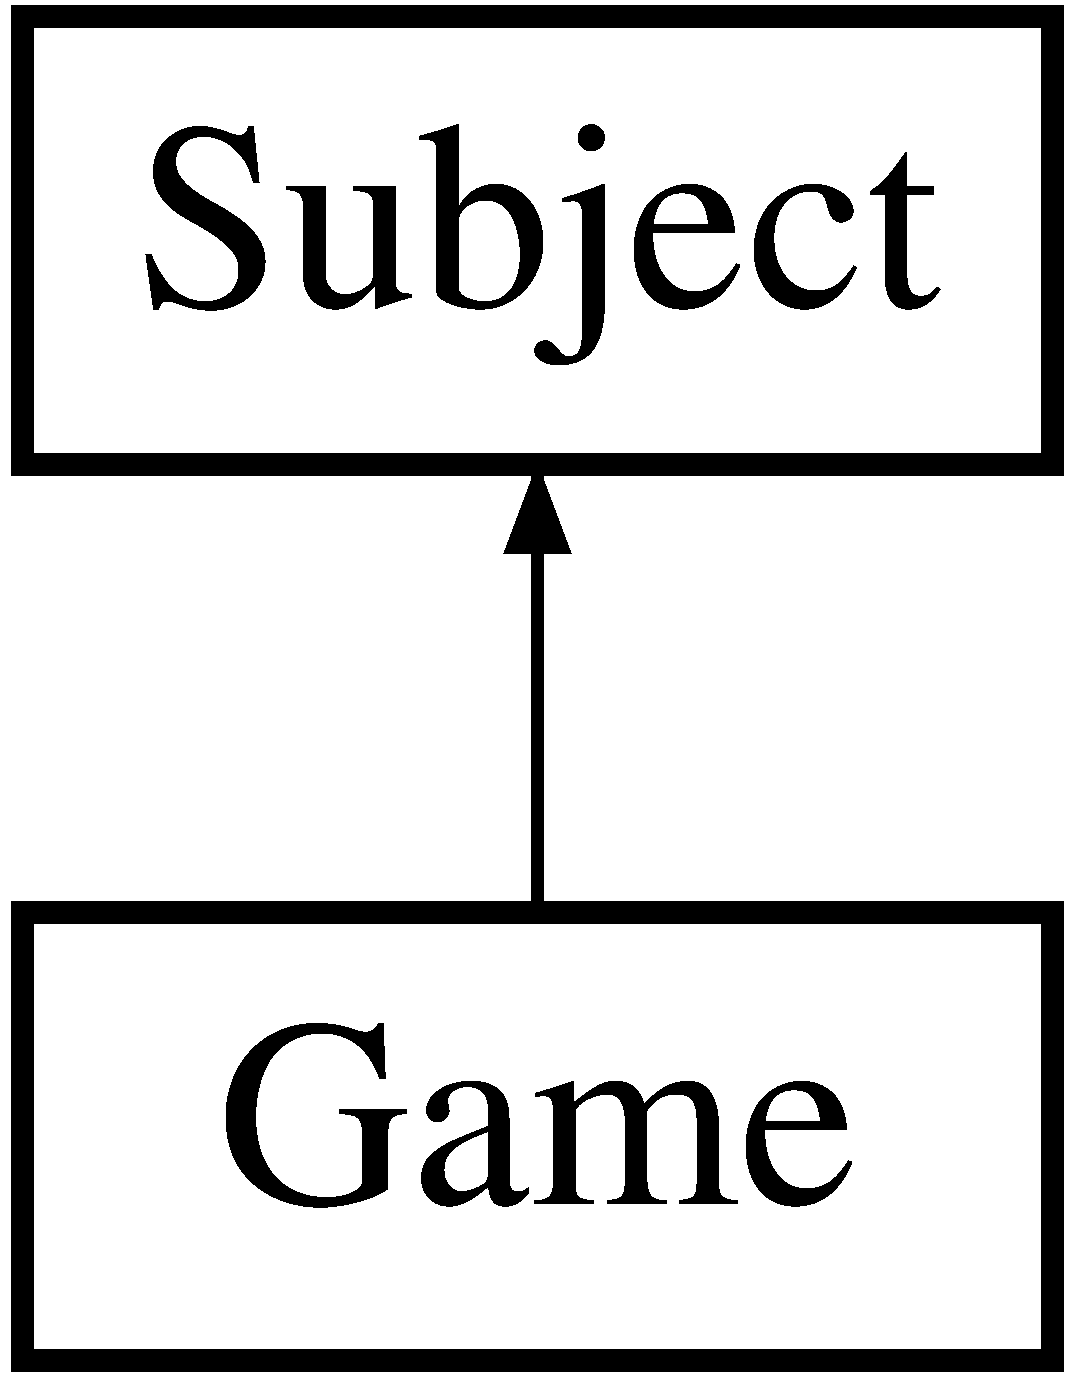
\includegraphics[height=2.000000cm]{classSubject}
\end{center}
\end{figure}
\subsection*{Fonctions membres publiques}
\begin{DoxyCompactItemize}
\item 
\hypertarget{classSubject_a4a12fdee2e95909a575066103986fa85}{virtual void \hyperlink{classSubject_a4a12fdee2e95909a575066103986fa85}{add\+Obs} (\hyperlink{classObserver}{Observer} $\ast$o)=0}\label{classSubject_a4a12fdee2e95909a575066103986fa85}

\begin{DoxyCompactList}\small\item\em ajout d'un observateur \end{DoxyCompactList}\item 
\hypertarget{classSubject_a1005f6c36e1a65fb13f1f0fa908b82e0}{virtual void \hyperlink{classSubject_a1005f6c36e1a65fb13f1f0fa908b82e0}{rm\+Obs} (\hyperlink{classObserver}{Observer} $\ast$o)=0}\label{classSubject_a1005f6c36e1a65fb13f1f0fa908b82e0}

\begin{DoxyCompactList}\small\item\em suppresion d'un observateur \end{DoxyCompactList}\item 
\hypertarget{classSubject_a421d620f3f93365bfd57cd1e9165e501}{virtual void \hyperlink{classSubject_a421d620f3f93365bfd57cd1e9165e501}{notify\+Obs} ()=0}\label{classSubject_a421d620f3f93365bfd57cd1e9165e501}

\begin{DoxyCompactList}\small\item\em notification de tous les observateurs \end{DoxyCompactList}\item 
\hypertarget{classSubject_ab847f18f48b243cf2104d7b8bc4fdb62}{virtual \hyperlink{classData}{Data} $\ast$ \hyperlink{classSubject_ab847f18f48b243cf2104d7b8bc4fdb62}{get\+Data} ()=0}\label{classSubject_ab847f18f48b243cf2104d7b8bc4fdb62}

\begin{DoxyCompactList}\small\item\em récupèration des données \end{DoxyCompactList}\item 
\hypertarget{classSubject_ac5639945604c72dc64e4a173bf60a516}{virtual \hyperlink{classMap}{Map} $\ast$ \hyperlink{classSubject_ac5639945604c72dc64e4a173bf60a516}{get\+Map} ()=0}\label{classSubject_ac5639945604c72dc64e4a173bf60a516}

\begin{DoxyCompactList}\small\item\em récupèration de la map \end{DoxyCompactList}\end{DoxyCompactItemize}


\subsection{Description détaillée}
Classe abstraite définissant le comportement des toutes les classes sujets. 

Définition à la ligne 22 du fichier subject.\+hpp.



La documentation de cette classe a été générée à partir du fichier suivant \+:\begin{DoxyCompactItemize}
\item 
src/\hyperlink{subject_8hpp}{subject.\+hpp}\end{DoxyCompactItemize}

\hypertarget{classTileMap}{\section{Référence de la classe Tile\+Map}
\label{classTileMap}\index{Tile\+Map@{Tile\+Map}}
}


Affichage d'une map.  




{\ttfamily \#include $<$tilemap.\+hpp$>$}

Graphe d'héritage de Tile\+Map\+:\begin{figure}[H]
\begin{center}
\leavevmode
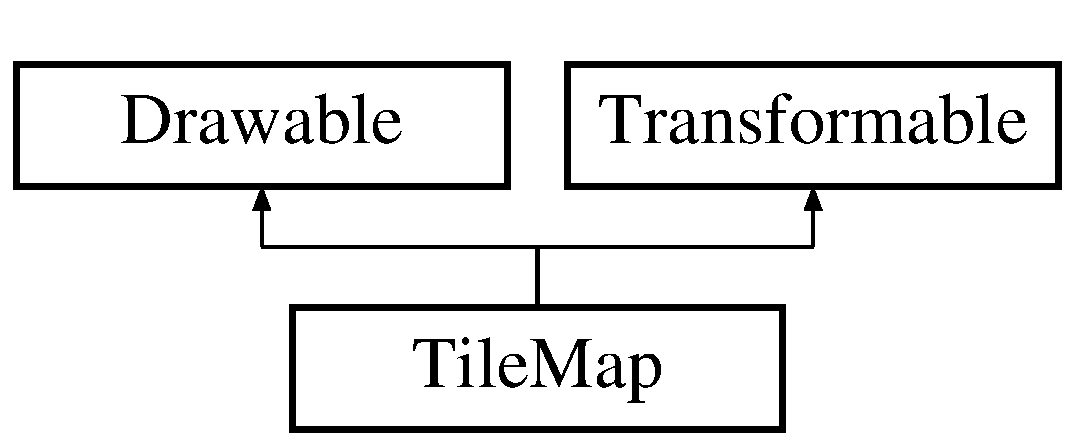
\includegraphics[height=2.000000cm]{classTileMap}
\end{center}
\end{figure}
\subsection*{Fonctions membres publiques}
\begin{DoxyCompactItemize}
\item 
\hypertarget{classTileMap_ac8af48f82359cb36b2db864c07278756}{bool {\bfseries load} (const std\+::string \&tileset, sf\+::\+Vector2u tile\+Size, std\+::vector$<$ std\+::vector$<$ unsigned int $>$$>$ tiles, unsigned int width, unsigned int height)}\label{classTileMap_ac8af48f82359cb36b2db864c07278756}

\end{DoxyCompactItemize}


\subsection{Description détaillée}
Affichage d'une map. 

Définition à la ligne 19 du fichier tilemap.\+hpp.



La documentation de cette classe a été générée à partir du fichier suivant \+:\begin{DoxyCompactItemize}
\item 
src/\hyperlink{tilemap_8hpp}{tilemap.\+hpp}\end{DoxyCompactItemize}

\hypertarget{classUnit}{\section{Référence de la classe Unit}
\label{classUnit}\index{Unit@{Unit}}
}


Classe permettant l'utilisation d'unités.  




{\ttfamily \#include $<$unit.\+hpp$>$}

Graphe d'héritage de Unit\+:\begin{figure}[H]
\begin{center}
\leavevmode
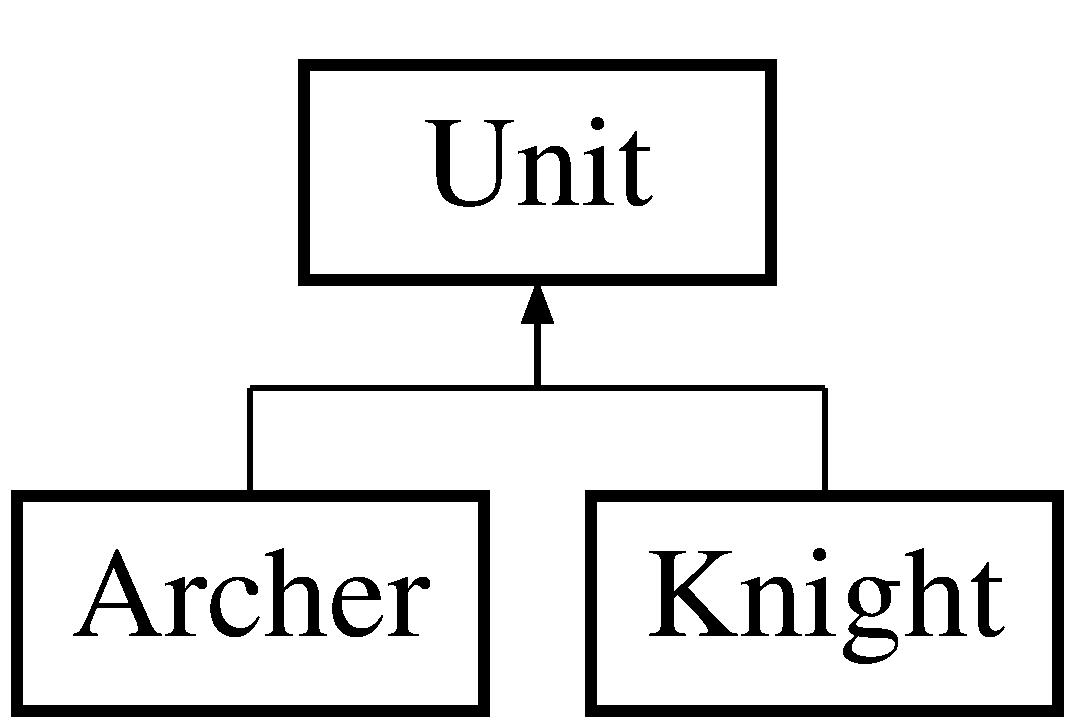
\includegraphics[height=2.000000cm]{classUnit}
\end{center}
\end{figure}
\subsection*{Fonctions membres publiques}
\begin{DoxyCompactItemize}
\item 
\hypertarget{classUnit_aa921e68cbe458d7cf65c8ba4c23bc162}{\hyperlink{classUnit_aa921e68cbe458d7cf65c8ba4c23bc162}{Unit} (unsigned int range, unsigned int ap, unsigned int mp, unsigned int hp, unsigned int dmgs, unsigned int cost, \hyperlink{classAttack}{Attack} $\ast$\hyperlink{classUnit_ac06b8f6e30f851f15a42d8a1d951034a}{attack}, \hyperlink{classHPLoss}{H\+P\+Loss} $\ast$\hyperlink{classUnit_a3090f43e2ee6a08587a160afaa26e7cd}{hp\+Loss}, \hyperlink{classMove}{Move} $\ast$\hyperlink{classUnit_a8c6bfbaf9bf204baec6ba3c11468ec2f}{move}, \hyperlink{classPosition}{Position} position, std\+::string image)}\label{classUnit_aa921e68cbe458d7cf65c8ba4c23bc162}

\begin{DoxyCompactList}\small\item\em Constructeur. \end{DoxyCompactList}\item 
unsigned int \hyperlink{classUnit_a5178a7baf2fb908a6232c3117af4bebd}{get\+Id} () const 
\begin{DoxyCompactList}\small\item\em Destructeur (évite les warnings) \end{DoxyCompactList}\item 
\hyperlink{classPosition}{Position} \hyperlink{classUnit_acf607fa2a07b1c50829c151a865ff4e6}{get\+Position} () const 
\begin{DoxyCompactList}\small\item\em Accesseur de la position. \end{DoxyCompactList}\item 
unsigned int \hyperlink{classUnit_a583b24bee2b519bb4b6feb94502c2645}{get\+Range} () const 
\begin{DoxyCompactList}\small\item\em Accesseur de la portée. \end{DoxyCompactList}\item 
unsigned int \hyperlink{classUnit_ac44844d1a66456789d803e157baf500d}{get\+A\+P} () const 
\begin{DoxyCompactList}\small\item\em Accesseur des points d'action. \end{DoxyCompactList}\item 
\hypertarget{classUnit_ac869149c544c48d375318e4d0f2f118f}{unsigned int {\bfseries get\+Max\+A\+P} () const }\label{classUnit_ac869149c544c48d375318e4d0f2f118f}

\item 
unsigned int \hyperlink{classUnit_ab63830d1bc4db11dc38634d5efe1401e}{get\+M\+P} () const 
\begin{DoxyCompactList}\small\item\em Accesseur des points de mouvement. \end{DoxyCompactList}\item 
\hypertarget{classUnit_ae8eea4bbc468f95b7ce52edddc37de53}{unsigned int {\bfseries get\+Max\+M\+P} () const }\label{classUnit_ae8eea4bbc468f95b7ce52edddc37de53}

\item 
unsigned int \hyperlink{classUnit_a2114b6ef6c9af9dddeb88aeddbc22043}{get\+H\+P} () const 
\begin{DoxyCompactList}\small\item\em Accesseur des points de vie. \end{DoxyCompactList}\item 
\hypertarget{classUnit_aa04fff8cffcb1da0e0fb4cbfda3e37d7}{unsigned int {\bfseries get\+Max\+H\+P} () const }\label{classUnit_aa04fff8cffcb1da0e0fb4cbfda3e37d7}

\item 
unsigned int \hyperlink{classUnit_a95d364646c70c571be6c010506a6eb42}{get\+Dmgs} () const 
\begin{DoxyCompactList}\small\item\em Accesseur des dommages. \end{DoxyCompactList}\item 
unsigned int \hyperlink{classUnit_a0fab4c57cd63d3a8c7019d074a645a87}{get\+Cost} () const 
\begin{DoxyCompactList}\small\item\em Accesseur du coût. \end{DoxyCompactList}\item 
std\+::string \hyperlink{classUnit_ab2c57e3a68452586ef2b2585efa75439}{get\+Image} () const 
\begin{DoxyCompactList}\small\item\em Accesseur de l'image. \end{DoxyCompactList}\item 
bool \hyperlink{classUnit_a1a6263ae2b5dea9d789e15ed8992b5df}{is\+Summoner} () const 
\begin{DoxyCompactList}\small\item\em Accesseur de la capacité Summoner. \end{DoxyCompactList}\item 
bool \hyperlink{classUnit_afb4ddd2c148dcedcf76767a38096fbe3}{is\+Builder} () const 
\begin{DoxyCompactList}\small\item\em Accesseur de la capacité Builder. \end{DoxyCompactList}\item 
\hypertarget{classUnit_a7b6b1b0eaebc2ac76b263aac194bcac4}{void \hyperlink{classUnit_a7b6b1b0eaebc2ac76b263aac194bcac4}{set\+Range} (unsigned int range)}\label{classUnit_a7b6b1b0eaebc2ac76b263aac194bcac4}

\begin{DoxyCompactList}\small\item\em Setter de portée. \end{DoxyCompactList}\item 
\hypertarget{classUnit_ab45c2fef4fe3a279a032dc9643247d17}{void \hyperlink{classUnit_ab45c2fef4fe3a279a032dc9643247d17}{set\+A\+P} (unsigned int ap)}\label{classUnit_ab45c2fef4fe3a279a032dc9643247d17}

\begin{DoxyCompactList}\small\item\em Setter de points d'action. \end{DoxyCompactList}\item 
\hypertarget{classUnit_a9f64ea3c64f8c19564640a37e97c9788}{void \hyperlink{classUnit_a9f64ea3c64f8c19564640a37e97c9788}{set\+M\+P} (unsigned int mp)}\label{classUnit_a9f64ea3c64f8c19564640a37e97c9788}

\begin{DoxyCompactList}\small\item\em Setter de points de mouvement. \end{DoxyCompactList}\item 
\hypertarget{classUnit_ae3a714e956dce20972b8f6384c319439}{void \hyperlink{classUnit_ae3a714e956dce20972b8f6384c319439}{set\+H\+P} (unsigned int hp)}\label{classUnit_ae3a714e956dce20972b8f6384c319439}

\begin{DoxyCompactList}\small\item\em Setter de points de vie. \end{DoxyCompactList}\item 
\hypertarget{classUnit_a9900634c53953be27d7e0bd2e00669b4}{void \hyperlink{classUnit_a9900634c53953be27d7e0bd2e00669b4}{set\+Dmgs} (unsigned int dmgs)}\label{classUnit_a9900634c53953be27d7e0bd2e00669b4}

\begin{DoxyCompactList}\small\item\em Setter de dommages. \end{DoxyCompactList}\item 
\hypertarget{classUnit_a518c16a1168ddde8fa3616dab1e034de}{void \hyperlink{classUnit_a518c16a1168ddde8fa3616dab1e034de}{set\+Position} (\hyperlink{classPosition}{Position} pos)}\label{classUnit_a518c16a1168ddde8fa3616dab1e034de}

\begin{DoxyCompactList}\small\item\em Setter de positon. \end{DoxyCompactList}\item 
\hypertarget{classUnit_a28a3e0beaa973c59fef271452117191c}{void \hyperlink{classUnit_a28a3e0beaa973c59fef271452117191c}{set\+Image} (std\+::string image)}\label{classUnit_a28a3e0beaa973c59fef271452117191c}

\begin{DoxyCompactList}\small\item\em Setter d'image. \end{DoxyCompactList}\item 
\hypertarget{classUnit_a9a35240ea4ccd698e65e4b466344a2cf}{void \hyperlink{classUnit_a9a35240ea4ccd698e65e4b466344a2cf}{set\+Summoner} ()}\label{classUnit_a9a35240ea4ccd698e65e4b466344a2cf}

\begin{DoxyCompactList}\small\item\em Setter de capacité Summoner ( la rend T\+R\+U\+E ) \end{DoxyCompactList}\item 
\hypertarget{classUnit_a9be2e7f4127fb29d7165f4f108a1e095}{void \hyperlink{classUnit_a9be2e7f4127fb29d7165f4f108a1e095}{set\+Builder} ()}\label{classUnit_a9be2e7f4127fb29d7165f4f108a1e095}

\begin{DoxyCompactList}\small\item\em Setter de capacité Builder ( la rend T\+R\+U\+E ) \end{DoxyCompactList}\item 
void \hyperlink{classUnit_ac06b8f6e30f851f15a42d8a1d951034a}{attack} (\hyperlink{classPosition}{Position} pos, \hyperlink{classMap}{Map} $\ast$map)
\begin{DoxyCompactList}\small\item\em L'unité attaque la position pos. \end{DoxyCompactList}\item 
void \hyperlink{classUnit_a3090f43e2ee6a08587a160afaa26e7cd}{hp\+Loss} (unsigned int value)
\begin{DoxyCompactList}\small\item\em L'unité perd des points de vie. \end{DoxyCompactList}\item 
void \hyperlink{classUnit_a8c6bfbaf9bf204baec6ba3c11468ec2f}{move} (\hyperlink{classPath}{Path} $\ast$path, \hyperlink{classMap}{Map} $\ast$map)
\begin{DoxyCompactList}\small\item\em Déplace l'unité \end{DoxyCompactList}\item 
\hypertarget{classUnit_adac07557f9c0b9005709c62263625c2d}{virtual std\+::string \hyperlink{classUnit_adac07557f9c0b9005709c62263625c2d}{classe} () const =0}\label{classUnit_adac07557f9c0b9005709c62263625c2d}

\begin{DoxyCompactList}\small\item\em Méthode virtuelle qui affiche le nom de la classe de l'unité \end{DoxyCompactList}\item 
\hypertarget{classUnit_a969abe2fc267339748d665c757991c33}{void \hyperlink{classUnit_a969abe2fc267339748d665c757991c33}{afficher} ()}\label{classUnit_a969abe2fc267339748d665c757991c33}

\begin{DoxyCompactList}\small\item\em Méthode qui affiche la classe de l'unité et sa position. \end{DoxyCompactList}\item 
virtual \hyperlink{classUnit}{Unit} $\ast$ \hyperlink{classUnit_a90304713be4b7cc73f59358190dd39d4}{clone} (\hyperlink{classPosition}{Position} position) const =0
\begin{DoxyCompactList}\small\item\em Méthode qui retourne une unité possèdant le même type, mais aussi les même caractéristiques que \char`\"{}this\char`\"{}. \end{DoxyCompactList}\item 
\hypertarget{classUnit_a21808f6976e0803ebdc1efcce18bd043}{virtual void \hyperlink{classUnit_a21808f6976e0803ebdc1efcce18bd043}{afficher\+Infos} () const =0}\label{classUnit_a21808f6976e0803ebdc1efcce18bd043}

\begin{DoxyCompactList}\small\item\em Affiche les infos de l'unité \end{DoxyCompactList}\item 
\hypertarget{classUnit_a2657eec715871bdfc44711526bcff5fa}{void \hyperlink{classUnit_a2657eec715871bdfc44711526bcff5fa}{end\+Turn} ()}\label{classUnit_a2657eec715871bdfc44711526bcff5fa}

\begin{DoxyCompactList}\small\item\em Méthode qui éxécute les actions de fin de tour comme réinitialiser les pa et pm. \end{DoxyCompactList}\end{DoxyCompactItemize}
\subsection*{Attributs protégés}
\begin{DoxyCompactItemize}
\item 
\hypertarget{classUnit_a4ec9562822eaba84e141ee30fc5d5561}{unsigned int {\bfseries \+\_\+id}}\label{classUnit_a4ec9562822eaba84e141ee30fc5d5561}

\item 
\hypertarget{classUnit_a7579bd13c0b683e3275ff84dcd39e614}{unsigned int {\bfseries \+\_\+range}}\label{classUnit_a7579bd13c0b683e3275ff84dcd39e614}

\item 
\hypertarget{classUnit_a968cd238d6ef530d33d2006a6dc80fba}{unsigned int {\bfseries \+\_\+ap}}\label{classUnit_a968cd238d6ef530d33d2006a6dc80fba}

\item 
\hypertarget{classUnit_aa5e25f6bb01279bf6909b631427fc3ae}{unsigned int {\bfseries \+\_\+ap\+Max}}\label{classUnit_aa5e25f6bb01279bf6909b631427fc3ae}

\item 
\hypertarget{classUnit_a84f6e9cf680ab7099e66caa5351ce79a}{unsigned int {\bfseries \+\_\+mp}}\label{classUnit_a84f6e9cf680ab7099e66caa5351ce79a}

\item 
\hypertarget{classUnit_a1fc6881c9ee518068f06636ff62d0a1c}{unsigned int {\bfseries \+\_\+mp\+Max}}\label{classUnit_a1fc6881c9ee518068f06636ff62d0a1c}

\item 
\hypertarget{classUnit_a59c016727ae555e75b61bc4b892d59c8}{unsigned int {\bfseries \+\_\+hp}}\label{classUnit_a59c016727ae555e75b61bc4b892d59c8}

\item 
\hypertarget{classUnit_abad6457e178bd9ca252256f5a18bd6a3}{unsigned int {\bfseries \+\_\+hp\+Max}}\label{classUnit_abad6457e178bd9ca252256f5a18bd6a3}

\item 
\hypertarget{classUnit_a9446a74a19fc662bc46d0a35651d6257}{unsigned int {\bfseries \+\_\+dmgs}}\label{classUnit_a9446a74a19fc662bc46d0a35651d6257}

\item 
\hypertarget{classUnit_a752100201cd0ce04b6a361068eaa65ec}{unsigned int {\bfseries \+\_\+cost}}\label{classUnit_a752100201cd0ce04b6a361068eaa65ec}

\item 
\hypertarget{classUnit_a6b77105078af83db82bfd4006a154e74}{\hyperlink{classPosition}{Position} {\bfseries \+\_\+position}}\label{classUnit_a6b77105078af83db82bfd4006a154e74}

\item 
\hypertarget{classUnit_ad6e87d9c5ea0823038a73cd725fc9b9c}{\hyperlink{classAttack}{Attack} $\ast$ {\bfseries \+\_\+attack}}\label{classUnit_ad6e87d9c5ea0823038a73cd725fc9b9c}

\item 
\hypertarget{classUnit_a1c139b04cef906782f4a96e520d9a898}{\hyperlink{classHPLoss}{H\+P\+Loss} $\ast$ {\bfseries \+\_\+hp\+Loss}}\label{classUnit_a1c139b04cef906782f4a96e520d9a898}

\item 
\hypertarget{classUnit_ad706684b8e916ef6a4df0c627a530afd}{\hyperlink{classMove}{Move} $\ast$ {\bfseries \+\_\+move}}\label{classUnit_ad706684b8e916ef6a4df0c627a530afd}

\item 
\hypertarget{classUnit_ab0e6ee2082c96facf7b6e297bb032e18}{bool {\bfseries \+\_\+summoner}}\label{classUnit_ab0e6ee2082c96facf7b6e297bb032e18}

\item 
\hypertarget{classUnit_a18e0ba8d6b5a45db49111dc5140cc634}{bool {\bfseries \+\_\+builder}}\label{classUnit_a18e0ba8d6b5a45db49111dc5140cc634}

\item 
\hypertarget{classUnit_a6760f1e268d6abe3413b5fd91d3c3c0f}{std\+::string {\bfseries \+\_\+image}}\label{classUnit_a6760f1e268d6abe3413b5fd91d3c3c0f}

\end{DoxyCompactItemize}
\subsection*{Attributs protégés statiques}
\begin{DoxyCompactItemize}
\item 
\hypertarget{classUnit_aff329e42743a57d23cd317dbbae9e4db}{static unsigned int {\bfseries \+\_\+next\+Id}}\label{classUnit_aff329e42743a57d23cd317dbbae9e4db}

\end{DoxyCompactItemize}


\subsection{Description détaillée}
Classe permettant l'utilisation d'unités. 

Définition à la ligne 26 du fichier unit.\+hpp.



\subsection{Documentation des fonctions membres}
\hypertarget{classUnit_ac06b8f6e30f851f15a42d8a1d951034a}{\index{Unit@{Unit}!attack@{attack}}
\index{attack@{attack}!Unit@{Unit}}
\subsubsection[{attack}]{\setlength{\rightskip}{0pt plus 5cm}void Unit\+::attack (
\begin{DoxyParamCaption}
\item[{{\bf Position}}]{pos, }
\item[{{\bf Map} $\ast$}]{map}
\end{DoxyParamCaption}
)}}\label{classUnit_ac06b8f6e30f851f15a42d8a1d951034a}


L'unité attaque la position pos. 


\begin{DoxyParams}{Paramètres}
{\em pos} & La position à attaquer \\
\hline
{\em map} & La carte \\
\hline
\end{DoxyParams}
\hypertarget{classUnit_a90304713be4b7cc73f59358190dd39d4}{\index{Unit@{Unit}!clone@{clone}}
\index{clone@{clone}!Unit@{Unit}}
\subsubsection[{clone}]{\setlength{\rightskip}{0pt plus 5cm}virtual {\bf Unit}$\ast$ Unit\+::clone (
\begin{DoxyParamCaption}
\item[{{\bf Position}}]{position}
\end{DoxyParamCaption}
) const\hspace{0.3cm}{\ttfamily [pure virtual]}}}\label{classUnit_a90304713be4b7cc73f59358190dd39d4}


Méthode qui retourne une unité possèdant le même type, mais aussi les même caractéristiques que \char`\"{}this\char`\"{}. 


\begin{DoxyParams}{Paramètres}
{\em position} & la position assignée à l'unité retournée \\
\hline
\end{DoxyParams}
\begin{DoxyReturn}{Renvoie}
un clone de \char`\"{}this\char`\"{} 
\end{DoxyReturn}


Implémenté dans \hyperlink{classArcher_a898839f83f972b3e2c000c9dfb92487c}{Archer}, et \hyperlink{classKnight_aff78fcbbd38c405b5c35f348160edce3}{Knight}.

\hypertarget{classUnit_ac44844d1a66456789d803e157baf500d}{\index{Unit@{Unit}!get\+A\+P@{get\+A\+P}}
\index{get\+A\+P@{get\+A\+P}!Unit@{Unit}}
\subsubsection[{get\+A\+P}]{\setlength{\rightskip}{0pt plus 5cm}unsigned int Unit\+::get\+A\+P (
\begin{DoxyParamCaption}
{}
\end{DoxyParamCaption}
) const}}\label{classUnit_ac44844d1a66456789d803e157baf500d}


Accesseur des points d'action. 

\begin{DoxyReturn}{Renvoie}
le nombre de P\+A 
\end{DoxyReturn}
\hypertarget{classUnit_a0fab4c57cd63d3a8c7019d074a645a87}{\index{Unit@{Unit}!get\+Cost@{get\+Cost}}
\index{get\+Cost@{get\+Cost}!Unit@{Unit}}
\subsubsection[{get\+Cost}]{\setlength{\rightskip}{0pt plus 5cm}unsigned int Unit\+::get\+Cost (
\begin{DoxyParamCaption}
{}
\end{DoxyParamCaption}
) const}}\label{classUnit_a0fab4c57cd63d3a8c7019d074a645a87}


Accesseur du coût. 

\begin{DoxyReturn}{Renvoie}
le coût 
\end{DoxyReturn}
\hypertarget{classUnit_a95d364646c70c571be6c010506a6eb42}{\index{Unit@{Unit}!get\+Dmgs@{get\+Dmgs}}
\index{get\+Dmgs@{get\+Dmgs}!Unit@{Unit}}
\subsubsection[{get\+Dmgs}]{\setlength{\rightskip}{0pt plus 5cm}unsigned int Unit\+::get\+Dmgs (
\begin{DoxyParamCaption}
{}
\end{DoxyParamCaption}
) const}}\label{classUnit_a95d364646c70c571be6c010506a6eb42}


Accesseur des dommages. 

\begin{DoxyReturn}{Renvoie}
les dommages 
\end{DoxyReturn}
\hypertarget{classUnit_a2114b6ef6c9af9dddeb88aeddbc22043}{\index{Unit@{Unit}!get\+H\+P@{get\+H\+P}}
\index{get\+H\+P@{get\+H\+P}!Unit@{Unit}}
\subsubsection[{get\+H\+P}]{\setlength{\rightskip}{0pt plus 5cm}unsigned int Unit\+::get\+H\+P (
\begin{DoxyParamCaption}
{}
\end{DoxyParamCaption}
) const}}\label{classUnit_a2114b6ef6c9af9dddeb88aeddbc22043}


Accesseur des points de vie. 

\begin{DoxyReturn}{Renvoie}
le nombre de H\+P 
\end{DoxyReturn}
\hypertarget{classUnit_a5178a7baf2fb908a6232c3117af4bebd}{\index{Unit@{Unit}!get\+Id@{get\+Id}}
\index{get\+Id@{get\+Id}!Unit@{Unit}}
\subsubsection[{get\+Id}]{\setlength{\rightskip}{0pt plus 5cm}unsigned int Unit\+::get\+Id (
\begin{DoxyParamCaption}
{}
\end{DoxyParamCaption}
) const}}\label{classUnit_a5178a7baf2fb908a6232c3117af4bebd}


Destructeur (évite les warnings) 

Accesseur de l'identifiant \begin{DoxyReturn}{Renvoie}
l'identifiant du décor 
\end{DoxyReturn}
\hypertarget{classUnit_ab2c57e3a68452586ef2b2585efa75439}{\index{Unit@{Unit}!get\+Image@{get\+Image}}
\index{get\+Image@{get\+Image}!Unit@{Unit}}
\subsubsection[{get\+Image}]{\setlength{\rightskip}{0pt plus 5cm}std\+::string Unit\+::get\+Image (
\begin{DoxyParamCaption}
{}
\end{DoxyParamCaption}
) const}}\label{classUnit_ab2c57e3a68452586ef2b2585efa75439}


Accesseur de l'image. 

\begin{DoxyReturn}{Renvoie}
l'image 
\end{DoxyReturn}
\hypertarget{classUnit_ab63830d1bc4db11dc38634d5efe1401e}{\index{Unit@{Unit}!get\+M\+P@{get\+M\+P}}
\index{get\+M\+P@{get\+M\+P}!Unit@{Unit}}
\subsubsection[{get\+M\+P}]{\setlength{\rightskip}{0pt plus 5cm}unsigned int Unit\+::get\+M\+P (
\begin{DoxyParamCaption}
{}
\end{DoxyParamCaption}
) const}}\label{classUnit_ab63830d1bc4db11dc38634d5efe1401e}


Accesseur des points de mouvement. 

\begin{DoxyReturn}{Renvoie}
le nombre de P\+M 
\end{DoxyReturn}
\hypertarget{classUnit_acf607fa2a07b1c50829c151a865ff4e6}{\index{Unit@{Unit}!get\+Position@{get\+Position}}
\index{get\+Position@{get\+Position}!Unit@{Unit}}
\subsubsection[{get\+Position}]{\setlength{\rightskip}{0pt plus 5cm}{\bf Position} Unit\+::get\+Position (
\begin{DoxyParamCaption}
{}
\end{DoxyParamCaption}
) const}}\label{classUnit_acf607fa2a07b1c50829c151a865ff4e6}


Accesseur de la position. 

\begin{DoxyReturn}{Renvoie}
la position du décor 
\end{DoxyReturn}
\hypertarget{classUnit_a583b24bee2b519bb4b6feb94502c2645}{\index{Unit@{Unit}!get\+Range@{get\+Range}}
\index{get\+Range@{get\+Range}!Unit@{Unit}}
\subsubsection[{get\+Range}]{\setlength{\rightskip}{0pt plus 5cm}unsigned int Unit\+::get\+Range (
\begin{DoxyParamCaption}
{}
\end{DoxyParamCaption}
) const}}\label{classUnit_a583b24bee2b519bb4b6feb94502c2645}


Accesseur de la portée. 

\begin{DoxyReturn}{Renvoie}
la portée d'attaque 
\end{DoxyReturn}
\hypertarget{classUnit_a3090f43e2ee6a08587a160afaa26e7cd}{\index{Unit@{Unit}!hp\+Loss@{hp\+Loss}}
\index{hp\+Loss@{hp\+Loss}!Unit@{Unit}}
\subsubsection[{hp\+Loss}]{\setlength{\rightskip}{0pt plus 5cm}void Unit\+::hp\+Loss (
\begin{DoxyParamCaption}
\item[{unsigned int}]{value}
\end{DoxyParamCaption}
)}}\label{classUnit_a3090f43e2ee6a08587a160afaa26e7cd}


L'unité perd des points de vie. 


\begin{DoxyParams}{Paramètres}
{\em value} & Le nomdre d'H\+P perdus \\
\hline
\end{DoxyParams}
\hypertarget{classUnit_afb4ddd2c148dcedcf76767a38096fbe3}{\index{Unit@{Unit}!is\+Builder@{is\+Builder}}
\index{is\+Builder@{is\+Builder}!Unit@{Unit}}
\subsubsection[{is\+Builder}]{\setlength{\rightskip}{0pt plus 5cm}bool Unit\+::is\+Builder (
\begin{DoxyParamCaption}
{}
\end{DoxyParamCaption}
) const}}\label{classUnit_afb4ddd2c148dcedcf76767a38096fbe3}


Accesseur de la capacité Builder. 

\begin{DoxyReturn}{Renvoie}
booléen V/\+F 
\end{DoxyReturn}
\hypertarget{classUnit_a1a6263ae2b5dea9d789e15ed8992b5df}{\index{Unit@{Unit}!is\+Summoner@{is\+Summoner}}
\index{is\+Summoner@{is\+Summoner}!Unit@{Unit}}
\subsubsection[{is\+Summoner}]{\setlength{\rightskip}{0pt plus 5cm}bool Unit\+::is\+Summoner (
\begin{DoxyParamCaption}
{}
\end{DoxyParamCaption}
) const}}\label{classUnit_a1a6263ae2b5dea9d789e15ed8992b5df}


Accesseur de la capacité Summoner. 

\begin{DoxyReturn}{Renvoie}
booléen V/\+F 
\end{DoxyReturn}
\hypertarget{classUnit_a8c6bfbaf9bf204baec6ba3c11468ec2f}{\index{Unit@{Unit}!move@{move}}
\index{move@{move}!Unit@{Unit}}
\subsubsection[{move}]{\setlength{\rightskip}{0pt plus 5cm}void Unit\+::move (
\begin{DoxyParamCaption}
\item[{{\bf Path} $\ast$}]{path, }
\item[{{\bf Map} $\ast$}]{map}
\end{DoxyParamCaption}
)}}\label{classUnit_a8c6bfbaf9bf204baec6ba3c11468ec2f}


Déplace l'unité 


\begin{DoxyParams}{Paramètres}
{\em path} & Le chemin emprunté \\
\hline
{\em map} & La carte \\
\hline
\end{DoxyParams}


La documentation de cette classe a été générée à partir du fichier suivant \+:\begin{DoxyCompactItemize}
\item 
src/\hyperlink{unit_8hpp}{unit.\+hpp}\end{DoxyCompactItemize}

\hypertarget{classWindow}{\section{Référence de la classe Window}
\label{classWindow}\index{Window@{Window}}
}


Affichage d'une fenêtre.  




{\ttfamily \#include $<$window.\+hpp$>$}

Graphe d'héritage de Window\+:\begin{figure}[H]
\begin{center}
\leavevmode
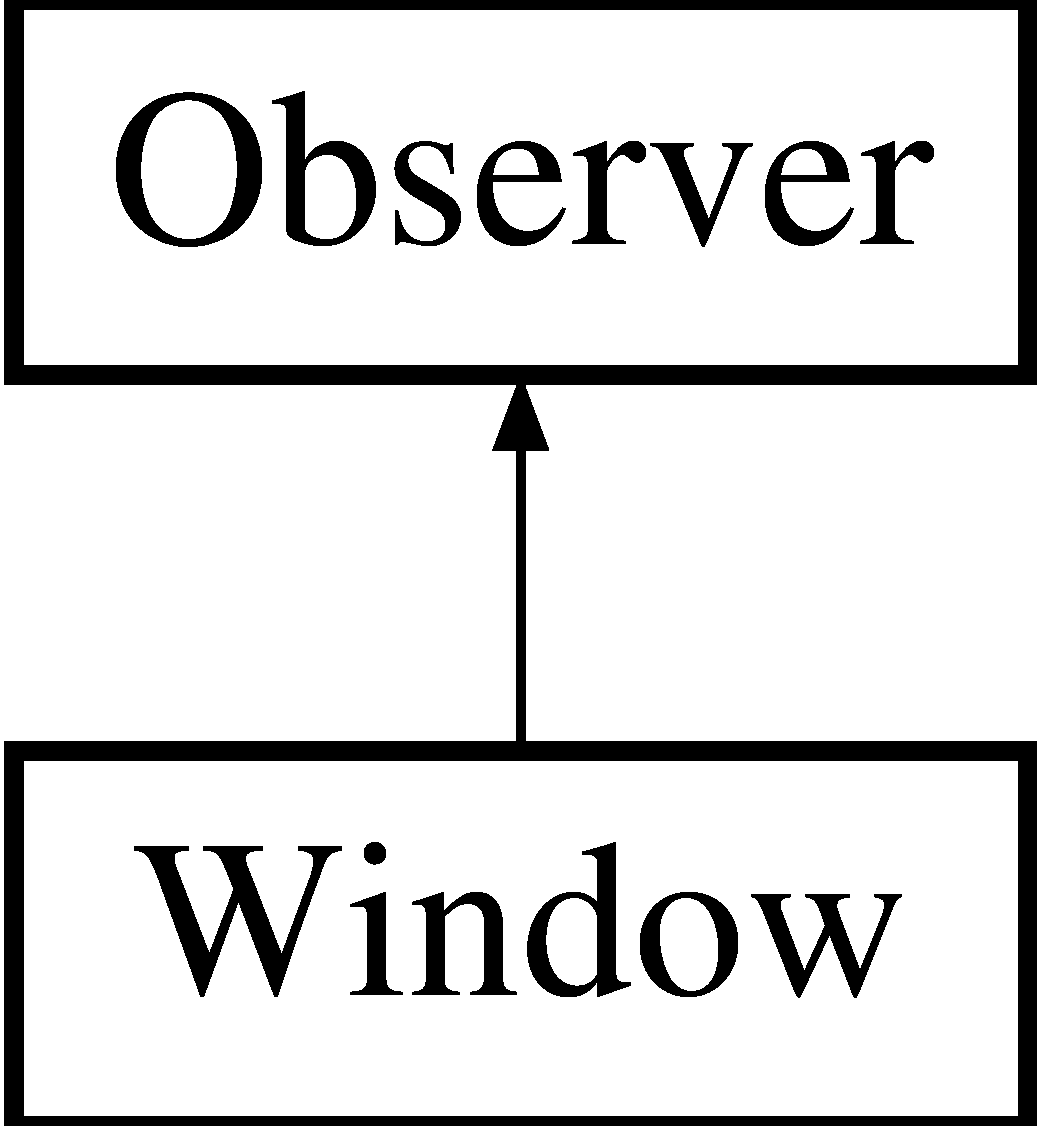
\includegraphics[height=2.000000cm]{classWindow}
\end{center}
\end{figure}
\subsection*{Fonctions membres publiques}
\begin{DoxyCompactItemize}
\item 
\hypertarget{classWindow_a2e2ce3cfbd3e468d389d8a9212e7b2ac}{\hyperlink{classWindow_a2e2ce3cfbd3e468d389d8a9212e7b2ac}{Window} (\hyperlink{classMap}{Map} $\ast$m)}\label{classWindow_a2e2ce3cfbd3e468d389d8a9212e7b2ac}

\begin{DoxyCompactList}\small\item\em Constructeur qui lance la fenêtre. \end{DoxyCompactList}\item 
void \hyperlink{classWindow_a23acb0c66756df8121ce5d54a8c28d72}{update} (\hyperlink{classSubject}{Subject} $\ast$s)
\begin{DoxyCompactList}\small\item\em Méthode d'update du pattern obervateur, met à jour la couleur du cercle. \end{DoxyCompactList}\item 
\hypertarget{classWindow_ad21ca1bd9a5c01411800f931bd7b1f7d}{void \hyperlink{classWindow_ad21ca1bd9a5c01411800f931bd7b1f7d}{quit} ()}\label{classWindow_ad21ca1bd9a5c01411800f931bd7b1f7d}

\begin{DoxyCompactList}\small\item\em Méthode qui ferme la fenêtre. \end{DoxyCompactList}\end{DoxyCompactItemize}


\subsection{Description détaillée}
Affichage d'une fenêtre. 

Définition à la ligne 24 du fichier window.\+hpp.



\subsection{Documentation des fonctions membres}
\hypertarget{classWindow_a23acb0c66756df8121ce5d54a8c28d72}{\index{Window@{Window}!update@{update}}
\index{update@{update}!Window@{Window}}
\subsubsection[{update}]{\setlength{\rightskip}{0pt plus 5cm}void Window\+::update (
\begin{DoxyParamCaption}
\item[{{\bf Subject} $\ast$}]{s}
\end{DoxyParamCaption}
)\hspace{0.3cm}{\ttfamily [virtual]}}}\label{classWindow_a23acb0c66756df8121ce5d54a8c28d72}


Méthode d'update du pattern obervateur, met à jour la couleur du cercle. 


\begin{DoxyParams}{Paramètres}
{\em s} & un sujet \\
\hline
\end{DoxyParams}


Implémente \hyperlink{classObserver_a27884af3c43e814cc1e613cd593efb55}{Observer}.



La documentation de cette classe a été générée à partir du fichier suivant \+:\begin{DoxyCompactItemize}
\item 
src/\hyperlink{window_8hpp}{window.\+hpp}\end{DoxyCompactItemize}

\chapter{Documentation des fichiers}
\hypertarget{archer_8hpp}{\section{Référence du fichier src/archer.hpp}
\label{archer_8hpp}\index{src/archer.\+hpp@{src/archer.\+hpp}}
}


Définition de la classe \hyperlink{classArcher}{Archer}.  


{\ttfamily \#include \char`\"{}unit.\+hpp\char`\"{}}\\*
{\ttfamily \#include $<$string$>$}\\*
\subsection*{Classes}
\begin{DoxyCompactItemize}
\item 
class \hyperlink{classArcher}{Archer}
\begin{DoxyCompactList}\small\item\em Classe définissant un archer. \end{DoxyCompactList}\end{DoxyCompactItemize}


\subsection{Description détaillée}
Définition de la classe \hyperlink{classArcher}{Archer}. 

\begin{DoxyAuthor}{Auteur}
B. Le Clère, A. Perhirin 
\end{DoxyAuthor}
\begin{DoxySince}{Depuis}
09/11/2015 
\end{DoxySince}


Définition dans le fichier \hyperlink{archer_8hpp_source}{archer.\+hpp}.


\hypertarget{attack_8hpp}{\section{Référence du fichier src/attack.hpp}
\label{attack_8hpp}\index{src/attack.\+hpp@{src/attack.\+hpp}}
}


Définition des stratégies d'attaque.  


\subsection*{Classes}
\begin{DoxyCompactItemize}
\item 
class \hyperlink{classAttack}{Attack}
\begin{DoxyCompactList}\small\item\em Classe virtuelle pure permettant l'utilisation de différents comportement d'attaque selon l'unité. Elle est utilisée dans le cadre du pattern Strategy. \end{DoxyCompactList}\end{DoxyCompactItemize}


\subsection{Description détaillée}
Définition des stratégies d'attaque. 

\begin{DoxyAuthor}{Auteur}
B. Le Clère, A. Perhirin 
\end{DoxyAuthor}
\begin{DoxySince}{Depuis}
05/10/2015 
\end{DoxySince}


Définition dans le fichier \hyperlink{attack_8hpp_source}{attack.\+hpp}.


\hypertarget{base_8hpp}{\section{Référence du fichier src/base.hpp}
\label{base_8hpp}\index{src/base.\+hpp@{src/base.\+hpp}}
}


Définition de la classe \hyperlink{classBase}{Base}.  


{\ttfamily \#include \char`\"{}position.\+hpp\char`\"{}}\\*
\subsection*{Classes}
\begin{DoxyCompactItemize}
\item 
class \hyperlink{classBase}{Base}
\begin{DoxyCompactList}\small\item\em Classe définissant une base. \end{DoxyCompactList}\end{DoxyCompactItemize}


\subsection{Description détaillée}
Définition de la classe \hyperlink{classBase}{Base}. 

\begin{DoxyAuthor}{Auteur}
B. Le Clère, A. Perhirin 
\end{DoxyAuthor}
\begin{DoxySince}{Depuis}
12/10/2015 
\end{DoxySince}


Définition dans le fichier \hyperlink{base_8hpp_source}{base.\+hpp}.


\hypertarget{concreteBaseAttack_8hpp}{\section{Référence du fichier src/concrete\+Base\+Attack.hpp}
\label{concreteBaseAttack_8hpp}\index{src/concrete\+Base\+Attack.\+hpp@{src/concrete\+Base\+Attack.\+hpp}}
}


Définition de l'attaque de base normale.  


{\ttfamily \#include \char`\"{}attack.\+hpp\char`\"{}}\\*
\subsection*{Classes}
\begin{DoxyCompactItemize}
\item 
class \hyperlink{classConcreteBaseAttack}{Concrete\+Base\+Attack}
\begin{DoxyCompactList}\small\item\em Classe concrete définissant le comportement d'attaque de base des unités normales. \end{DoxyCompactList}\end{DoxyCompactItemize}


\subsection{Description détaillée}
Définition de l'attaque de base normale. 

\begin{DoxyAuthor}{Auteur}
B. Le Clère, A. Perhirin 
\end{DoxyAuthor}
\begin{DoxySince}{Depuis}
19/10/2015 
\end{DoxySince}


Définition dans le fichier \hyperlink{concreteBaseAttack_8hpp_source}{concrete\+Base\+Attack.\+hpp}.


\hypertarget{concreteBaseAttackSpeBase_8hpp}{\section{Référence du fichier src/concrete\+Base\+Attack\+Spe\+Base.hpp}
\label{concreteBaseAttackSpeBase_8hpp}\index{src/concrete\+Base\+Attack\+Spe\+Base.\+hpp@{src/concrete\+Base\+Attack\+Spe\+Base.\+hpp}}
}


Définition de l'attaque de base pour les unité puissante sur les bases.  


{\ttfamily \#include \char`\"{}attack.\+hpp\char`\"{}}\\*
\subsection*{Classes}
\begin{DoxyCompactItemize}
\item 
class \hyperlink{classConcreteBaseAttackSpeBase}{Concrete\+Base\+Attack\+Spe\+Base}
\end{DoxyCompactItemize}


\subsection{Description détaillée}
Définition de l'attaque de base pour les unité puissante sur les bases. 

\begin{DoxyAuthor}{Auteur}
B. Le Clère, A. Perhirin 
\end{DoxyAuthor}
\begin{DoxySince}{Depuis}
19/10/2015 
\end{DoxySince}


Définition dans le fichier \hyperlink{concreteBaseAttackSpeBase_8hpp_source}{concrete\+Base\+Attack\+Spe\+Base.\+hpp}.


\hypertarget{concretehploss_8hpp}{\section{Référence du fichier src/concretehploss.hpp}
\label{concretehploss_8hpp}\index{src/concretehploss.\+hpp@{src/concretehploss.\+hpp}}
}


Définition de la perte d'H\+P de base.  


{\ttfamily \#include \char`\"{}hploss.\+hpp\char`\"{}}\\*
\subsection*{Classes}
\begin{DoxyCompactItemize}
\item 
class \hyperlink{classConcreteHPLoss}{Concrete\+H\+P\+Loss}
\end{DoxyCompactItemize}


\subsection{Description détaillée}
Définition de la perte d'H\+P de base. 

\begin{DoxyAuthor}{Auteur}
B. Le Clère, A. Perhirin 
\end{DoxyAuthor}
\begin{DoxySince}{Depuis}
19/10/2015 
\end{DoxySince}


Définition dans le fichier \hyperlink{concretehploss_8hpp_source}{concretehploss.\+hpp}.


\hypertarget{concretehplossspedef_8hpp}{\section{Référence du fichier src/concretehplossspedef.hpp}
\label{concretehplossspedef_8hpp}\index{src/concretehplossspedef.\+hpp@{src/concretehplossspedef.\+hpp}}
}


Définition de la perte d'H\+P d'une unité défensive.  


{\ttfamily \#include \char`\"{}hploss.\+hpp\char`\"{}}\\*
\subsection*{Classes}
\begin{DoxyCompactItemize}
\item 
class \hyperlink{classConcreteHPLossSpeDef}{Concrete\+H\+P\+Loss\+Spe\+Def}
\end{DoxyCompactItemize}


\subsection{Description détaillée}
Définition de la perte d'H\+P d'une unité défensive. 

\begin{DoxyAuthor}{Auteur}
B. Le Clère, A. Perhirin 
\end{DoxyAuthor}
\begin{DoxySince}{Depuis}
19/10/2015 
\end{DoxySince}


Définition dans le fichier \hyperlink{concretehplossspedef_8hpp_source}{concretehplossspedef.\+hpp}.


\hypertarget{concretemove_8hpp}{\section{Référence du fichier src/concretemove.hpp}
\label{concretemove_8hpp}\index{src/concretemove.\+hpp@{src/concretemove.\+hpp}}
}


Définition du mouvement.  


{\ttfamily \#include \char`\"{}move.\+hpp\char`\"{}}\\*
\subsection*{Classes}
\begin{DoxyCompactItemize}
\item 
class \hyperlink{classConcreteMove}{Concrete\+Move}
\begin{DoxyCompactList}\small\item\em Classe concrete définissant le comportement de déplacement des unités mouvantes. \end{DoxyCompactList}\end{DoxyCompactItemize}


\subsection{Description détaillée}
Définition du mouvement. 

\begin{DoxyAuthor}{Auteur}
B. Le Clère, A. Perhirin 
\end{DoxyAuthor}
\begin{DoxySince}{Depuis}
19/10/2015 
\end{DoxySince}


Définition dans le fichier \hyperlink{concretemove_8hpp_source}{concretemove.\+hpp}.


\hypertarget{data_8hpp}{\section{Référence du fichier src/data.hpp}
\label{data_8hpp}\index{src/data.\+hpp@{src/data.\+hpp}}
}


Définition de la classe data.  


{\ttfamily \#include $<$map$>$}\\*
{\ttfamily \#include $<$vector$>$}\\*
\subsection*{Classes}
\begin{DoxyCompactItemize}
\item 
class \hyperlink{classData}{Data}
\begin{DoxyCompactList}\small\item\em Classe qui centralise toute les données du jeu. \end{DoxyCompactList}\end{DoxyCompactItemize}


\subsection{Description détaillée}
Définition de la classe data. 

\begin{DoxyAuthor}{Auteur}
B. Le Clère, A. Perhirin 
\end{DoxyAuthor}
\begin{DoxySince}{Depuis}
03/11/2015 
\end{DoxySince}


Définition dans le fichier \hyperlink{data_8hpp_source}{data.\+hpp}.


\hypertarget{game_8hpp}{\section{Référence du fichier src/game.hpp}
\label{game_8hpp}\index{src/game.\+hpp@{src/game.\+hpp}}
}


Définition de la classe game.  


{\ttfamily \#include \char`\"{}subject.\+hpp\char`\"{}}\\*
{\ttfamily \#include $<$list$>$}\\*
{\ttfamily \#include $<$vector$>$}\\*
{\ttfamily \#include $<$iterator$>$}\\*
{\ttfamily \#include $<$string$>$}\\*
\subsection*{Classes}
\begin{DoxyCompactItemize}
\item 
class \hyperlink{classGame}{Game}
\begin{DoxyCompactList}\small\item\em Classe qui centralisera tout le jeu. \end{DoxyCompactList}\end{DoxyCompactItemize}


\subsection{Description détaillée}
Définition de la classe game. 

\begin{DoxyAuthor}{Auteur}
B. Le Clère, A. Perhirin 
\end{DoxyAuthor}
\begin{DoxySince}{Depuis}
03/11/2015 
\end{DoxySince}


Définition dans le fichier \hyperlink{game_8hpp_source}{game.\+hpp}.


\hypertarget{hploss_8hpp}{\section{Référence du fichier src/hploss.hpp}
\label{hploss_8hpp}\index{src/hploss.\+hpp@{src/hploss.\+hpp}}
}


Définition du comportement de la perte d'H\+P.  


\subsection*{Classes}
\begin{DoxyCompactItemize}
\item 
class \hyperlink{classHPLoss}{H\+P\+Loss}
\begin{DoxyCompactList}\small\item\em Classe virtuelle pure permettant l'utilisation de différents comportement de la perte de points de vie selon l'unité. Elle est utilisée dans le cadre du pattern Strategy. \end{DoxyCompactList}\end{DoxyCompactItemize}


\subsection{Description détaillée}
Définition du comportement de la perte d'H\+P. 

\begin{DoxyAuthor}{Auteur}
B. Le Clère, A. Perhirin 
\end{DoxyAuthor}
\begin{DoxySince}{Depuis}
05/10/2015 
\end{DoxySince}


Définition dans le fichier \hyperlink{hploss_8hpp_source}{hploss.\+hpp}.


\hypertarget{knight_8hpp}{\section{Référence du fichier src/knight.hpp}
\label{knight_8hpp}\index{src/knight.\+hpp@{src/knight.\+hpp}}
}


Définition de la classe \hyperlink{classKnight}{Knight}.  


{\ttfamily \#include $<$string$>$}\\*
{\ttfamily \#include \char`\"{}unit.\+hpp\char`\"{}}\\*
\subsection*{Classes}
\begin{DoxyCompactItemize}
\item 
class \hyperlink{classKnight}{Knight}
\begin{DoxyCompactList}\small\item\em Classe définissant un chevalier. \end{DoxyCompactList}\end{DoxyCompactItemize}


\subsection{Description détaillée}
Définition de la classe \hyperlink{classKnight}{Knight}. 

\begin{DoxyAuthor}{Auteur}
B. Le Clère, A. Perhirin 
\end{DoxyAuthor}
\begin{DoxySince}{Depuis}
12/10/2015 
\end{DoxySince}


Définition dans le fichier \hyperlink{knight_8hpp_source}{knight.\+hpp}.


\hypertarget{map_8hpp}{\section{Référence du fichier src/map.hpp}
\label{map_8hpp}\index{src/map.\+hpp@{src/map.\+hpp}}
}


Définition de la classe \hyperlink{classMap}{Map}.  


{\ttfamily \#include \char`\"{}position.\+hpp\char`\"{}}\\*
{\ttfamily \#include $<$map$>$}\\*
{\ttfamily \#include $<$vector$>$}\\*
\subsection*{Classes}
\begin{DoxyCompactItemize}
\item 
class \hyperlink{classMap}{Map}
\begin{DoxyCompactList}\small\item\em Classe permettant l'utilisation d'une map. \end{DoxyCompactList}\end{DoxyCompactItemize}


\subsection{Description détaillée}
Définition de la classe \hyperlink{classMap}{Map}. 

\begin{DoxyAuthor}{Auteur}
B. Le Clère, A. Perhirin 
\end{DoxyAuthor}
\begin{DoxySince}{Depuis}
07/10/2015 
\end{DoxySince}


Définition dans le fichier \hyperlink{map_8hpp_source}{map.\+hpp}.


\hypertarget{move_8hpp}{\section{Référence du fichier src/move.hpp}
\label{move_8hpp}\index{src/move.\+hpp@{src/move.\+hpp}}
}


Définition des stratégies de déplacement.  


\subsection*{Classes}
\begin{DoxyCompactItemize}
\item 
class \hyperlink{classMove}{Move}
\begin{DoxyCompactList}\small\item\em Classe virtuelle pure permettant l'utilisation de différents comportement de déplacements selon l'unité. Elle est utilisée dans le cadre du pattern Strategy. \end{DoxyCompactList}\end{DoxyCompactItemize}


\subsection{Description détaillée}
Définition des stratégies de déplacement. 

\begin{DoxyAuthor}{Auteur}
B. Le Clère, A. Perhirin 
\end{DoxyAuthor}
\begin{DoxySince}{Depuis}
05/10/2015 
\end{DoxySince}


Définition dans le fichier \hyperlink{move_8hpp_source}{move.\+hpp}.


\hypertarget{observer_8hpp}{\section{Référence du fichier src/observer.hpp}
\label{observer_8hpp}\index{src/observer.\+hpp@{src/observer.\+hpp}}
}


Définition de la classe abstraite observateur.  


\subsection*{Classes}
\begin{DoxyCompactItemize}
\item 
class \hyperlink{classObserver}{Observer}
\end{DoxyCompactItemize}


\subsection{Description détaillée}
Définition de la classe abstraite observateur. 

\begin{DoxyAuthor}{Auteur}
B. Le Clère A. Perhirin 
\end{DoxyAuthor}
\begin{DoxySince}{Depuis}
11/11/2015 
\end{DoxySince}


Définition dans le fichier \hyperlink{observer_8hpp_source}{observer.\+hpp}.


\hypertarget{path_8hpp}{\section{Référence du fichier src/path.hpp}
\label{path_8hpp}\index{src/path.\+hpp@{src/path.\+hpp}}
}


definition de la classe \hyperlink{classPath}{Path}  


{\ttfamily \#include \char`\"{}position.\+hpp\char`\"{}}\\*
{\ttfamily \#include $<$vector$>$}\\*
\subsection*{Classes}
\begin{DoxyCompactItemize}
\item 
class \hyperlink{classPath}{Path}
\begin{DoxyCompactList}\small\item\em Classe implémentant un chemin (path) sur la map. \end{DoxyCompactList}\end{DoxyCompactItemize}


\subsection{Description détaillée}
definition de la classe \hyperlink{classPath}{Path} 

\begin{DoxyAuthor}{Auteur}
A. Perhirin B. Le Clère 
\end{DoxyAuthor}
\begin{DoxyDate}{Date}
6/10/2015 
\end{DoxyDate}


Définition dans le fichier \hyperlink{path_8hpp_source}{path.\+hpp}.


\hypertarget{player_8hpp}{\section{Référence du fichier src/player.hpp}
\label{player_8hpp}\index{src/player.\+hpp@{src/player.\+hpp}}
}


Définition de la classe \hyperlink{classPlayer}{Player}.  


{\ttfamily \#include $<$map$>$}\\*
\subsection*{Classes}
\begin{DoxyCompactItemize}
\item 
class \hyperlink{classPlayer}{Player}
\begin{DoxyCompactList}\small\item\em Classe définissant un joueur. \end{DoxyCompactList}\end{DoxyCompactItemize}


\subsection{Description détaillée}
Définition de la classe \hyperlink{classPlayer}{Player}. 

\begin{DoxyAuthor}{Auteur}
B. Le Clère, A. Perhirin 
\end{DoxyAuthor}
\begin{DoxySince}{Depuis}
12/10/2015 
\end{DoxySince}


Définition dans le fichier \hyperlink{player_8hpp_source}{player.\+hpp}.


\hypertarget{position_8hpp}{\section{Référence du fichier src/position.hpp}
\label{position_8hpp}\index{src/position.\+hpp@{src/position.\+hpp}}
}


definition de la classe \hyperlink{classPosition}{Position}  


\subsection*{Classes}
\begin{DoxyCompactItemize}
\item 
class \hyperlink{classPosition}{Position}
\begin{DoxyCompactList}\small\item\em Classe implémentant une position sur la map. \end{DoxyCompactList}\end{DoxyCompactItemize}


\subsection{Description détaillée}
definition de la classe \hyperlink{classPosition}{Position} 

\begin{DoxyAuthor}{Auteur}
A. Perhirin B. Le Clère 
\end{DoxyAuthor}
\begin{DoxyDate}{Date}
5/10/2015 
\end{DoxyDate}


Définition dans le fichier \hyperlink{position_8hpp_source}{position.\+hpp}.


\hypertarget{spawner_8hpp}{\section{Référence du fichier src/spawner.hpp}
\label{spawner_8hpp}\index{src/spawner.\+hpp@{src/spawner.\+hpp}}
}


Définition de la classe \hyperlink{classSpawner}{Spawner}.  


\subsection*{Classes}
\begin{DoxyCompactItemize}
\item 
class \hyperlink{classSpawner}{Spawner}
\begin{DoxyCompactList}\small\item\em Classe permettant l'utilisation des spawner (générateur d'unités) \end{DoxyCompactList}\end{DoxyCompactItemize}


\subsection{Description détaillée}
Définition de la classe \hyperlink{classSpawner}{Spawner}. 

\begin{DoxyAuthor}{Auteur}
B. Le Clère, A. Perhirin 
\end{DoxyAuthor}
\begin{DoxySince}{Depuis}
06/11/2015 
\end{DoxySince}


Définition dans le fichier \hyperlink{spawner_8hpp_source}{spawner.\+hpp}.


\hypertarget{subject_8hpp}{\section{Référence du fichier src/subject.hpp}
\label{subject_8hpp}\index{src/subject.\+hpp@{src/subject.\+hpp}}
}


Définition de la classe abstraite sujet.  


{\ttfamily \#include $<$vector$>$}\\*
\subsection*{Classes}
\begin{DoxyCompactItemize}
\item 
class \hyperlink{classSubject}{Subject}
\begin{DoxyCompactList}\small\item\em Classe abstraite définissant le comportement des toutes les classes sujets. \end{DoxyCompactList}\end{DoxyCompactItemize}


\subsection{Description détaillée}
Définition de la classe abstraite sujet. 

\begin{DoxyAuthor}{Auteur}
B. Le Clère A. Perhirin 
\end{DoxyAuthor}
\begin{DoxySince}{Depuis}
11/11/2015 
\end{DoxySince}


Définition dans le fichier \hyperlink{subject_8hpp_source}{subject.\+hpp}.


\hypertarget{tilemap_8hpp}{\section{Référence du fichier src/tilemap.hpp}
\label{tilemap_8hpp}\index{src/tilemap.\+hpp@{src/tilemap.\+hpp}}
}


Définition de la classe qui crée la map graphique.  


{\ttfamily \#include $<$S\+F\+M\+L/\+Graphics.\+hpp$>$}\\*
{\ttfamily \#include $<$vector$>$}\\*
\subsection*{Classes}
\begin{DoxyCompactItemize}
\item 
class \hyperlink{classTileMap}{Tile\+Map}
\begin{DoxyCompactList}\small\item\em Affichage d'une map. \end{DoxyCompactList}\end{DoxyCompactItemize}


\subsection{Description détaillée}
Définition de la classe qui crée la map graphique. 

\begin{DoxyAuthor}{Auteur}
B. Le Clère A.\+Perhirin 
\end{DoxyAuthor}
\begin{DoxySince}{Depuis}
11/11/2015 
\end{DoxySince}


Définition dans le fichier \hyperlink{tilemap_8hpp_source}{tilemap.\+hpp}.


\hypertarget{unit_8hpp}{\section{Référence du fichier src/unit.hpp}
\label{unit_8hpp}\index{src/unit.\+hpp@{src/unit.\+hpp}}
}


Définition de la classe \hyperlink{classUnit}{Unit}.  


{\ttfamily \#include \char`\"{}position.\+hpp\char`\"{}}\\*
{\ttfamily \#include $<$string$>$}\\*
\subsection*{Classes}
\begin{DoxyCompactItemize}
\item 
class \hyperlink{classUnit}{Unit}
\begin{DoxyCompactList}\small\item\em Classe permettant l'utilisation d'unités. \end{DoxyCompactList}\end{DoxyCompactItemize}


\subsection{Description détaillée}
Définition de la classe \hyperlink{classUnit}{Unit}. 

\begin{DoxyAuthor}{Auteur}
B. Le Clère, A. Perhirin 
\end{DoxyAuthor}
\begin{DoxySince}{Depuis}
12/10/2015 
\end{DoxySince}


Définition dans le fichier \hyperlink{unit_8hpp_source}{unit.\+hpp}.


\hypertarget{window_8hpp}{\section{Référence du fichier src/window.hpp}
\label{window_8hpp}\index{src/window.\+hpp@{src/window.\+hpp}}
}


Définition de la classe d'affichage.  


{\ttfamily \#include \char`\"{}observer.\+hpp\char`\"{}}\\*
{\ttfamily \#include $<$vector$>$}\\*
{\ttfamily \#include $<$S\+F\+M\+L/\+Graphics.\+hpp$>$}\\*
\subsection*{Classes}
\begin{DoxyCompactItemize}
\item 
class \hyperlink{classWindow}{Window}
\begin{DoxyCompactList}\small\item\em Affichage d'une fenêtre. \end{DoxyCompactList}\end{DoxyCompactItemize}


\subsection{Description détaillée}
Définition de la classe d'affichage. 

\begin{DoxyAuthor}{Auteur}
B. Le Clère A.\+Perhirin 
\end{DoxyAuthor}
\begin{DoxySince}{Depuis}
11/11/2015 
\end{DoxySince}


Définition dans le fichier \hyperlink{window_8hpp_source}{window.\+hpp}.


%--- End generated contents ---

% Index
\newpage
\phantomsection
\addcontentsline{toc}{chapter}{Index}
\printindex

\end{document}
